\documentclass[12pt]{book}
\usepackage[dvipsnames]{xcolor}
\usepackage{amssymb,latexsym}
\usepackage{graphicx}
\usepackage{listings}
\usepackage{xcolor}
\usepackage[spanish,mexico,es-nolayout]{babel}
\usepackage[latin1]{inputenc}
\usepackage[spanish]{babel}
\usepackage{amsmath}
\usepackage{mdframed}
\usepackage{algorithm}
\usepackage{algorithmic}
\DeclareMathOperator{\tr}{tr}
% \usepackage{amssymb}
\usepackage{amsthm}
%\usepackage{graphicx}
\usepackage{color}
\usepackage{tikz}
\usepackage{tkz-berge}
\usetikzlibrary{positioning,backgrounds}
\usepackage{makeidx}
\usepackage{url}
\usepackage{xspace}
\usepackage{tocbibind}
\usepackage{rotating}
\usepackage{float}
\usepackage{young}
\usepackage{ytableau}
\usepackage{mathtools}
\DeclarePairedDelimiter\ceil{\lceil}{\rceil}
\DeclarePairedDelimiter\floor{\lfloor}{\rfloor}
% ver http://gilmation.com/articles/latex-margins-for-book-binding/
% y http://tex.stackexchange.com/questions/50258/margins-of-book-class
\usepackage[margin=3.5cm]{geometry}
\geometry{bindingoffset=1cm}

%\usepackage{babelbib}

\usetikzlibrary{positioning,shapes,fit,arrows,decorations.pathmorphing}
\definecolor{myblue}{RGB}{56,94,141}


\newtheorem{theorem}{Teorema}[section]
\newtheorem{corollary}[theorem]{Corolario}
\newtheorem{proposition}[theorem]{Proposición}

\theoremstyle{definition}

\newtheorem{definition}[theorem]{Definición}
\newtheorem{notation}[theorem]{Notación}
\newtheorem{example}[theorem]{Ejemplo}
\newtheorem{lemma}[theorem]{Lema}

\newcounter{in}
\newcounter{ini}

\DeclareMathOperator{\Cay}{Cay}
\DeclareMathOperator{\diam}{diam}
\DeclareMathOperator{\Stab}{Stab}
\DeclareMathOperator{\Aut}{Aut}
\DeclareMathOperator{\orb}{Orb}
\DeclareMathOperator{\im}{im}

\newcommand{\GAP}{\textsf{GAP}\xspace}
\newcommand{\GRAPE}{\textsf{GRAPE}\xspace}

\makeindex

\newcommand{\elespacio}{1.4cm}

\newcommand{\rep}{A}
%New colors defined below
\definecolor{codegreen}{rgb}{0,0.6,0}
\definecolor{codegray}{rgb}{0.5,0.5,0.5}
\definecolor{codepurple}{rgb}{0.58,0,0.82}
\definecolor{backcolour}{rgb}{0.95,0.95,0.92}

%Code listing style named "mystyle"
\lstdefinestyle{mystyle}{
  backgroundcolor=\color{backcolour},   commentstyle=\color{codegreen},
  keywordstyle=\color{magenta},
  numberstyle=\tiny\color{codegray},
  stringstyle=\color{codepurple},
  basicstyle=\ttfamily\footnotesize,
  breakatwhitespace=false,         
  breaklines=true,                 
  captionpos=b,                    
  keepspaces=true,                 
  numbers=left,                    
  numbersep=5pt,                  
  showspaces=false,                
  showstringspaces=false,
  showtabs=false,                  
  tabsize=2
}
\begin{document}
\mainmatter 
\begin{titlepage}
  \begin{center}
    \null
    \vspace*{\fill}

    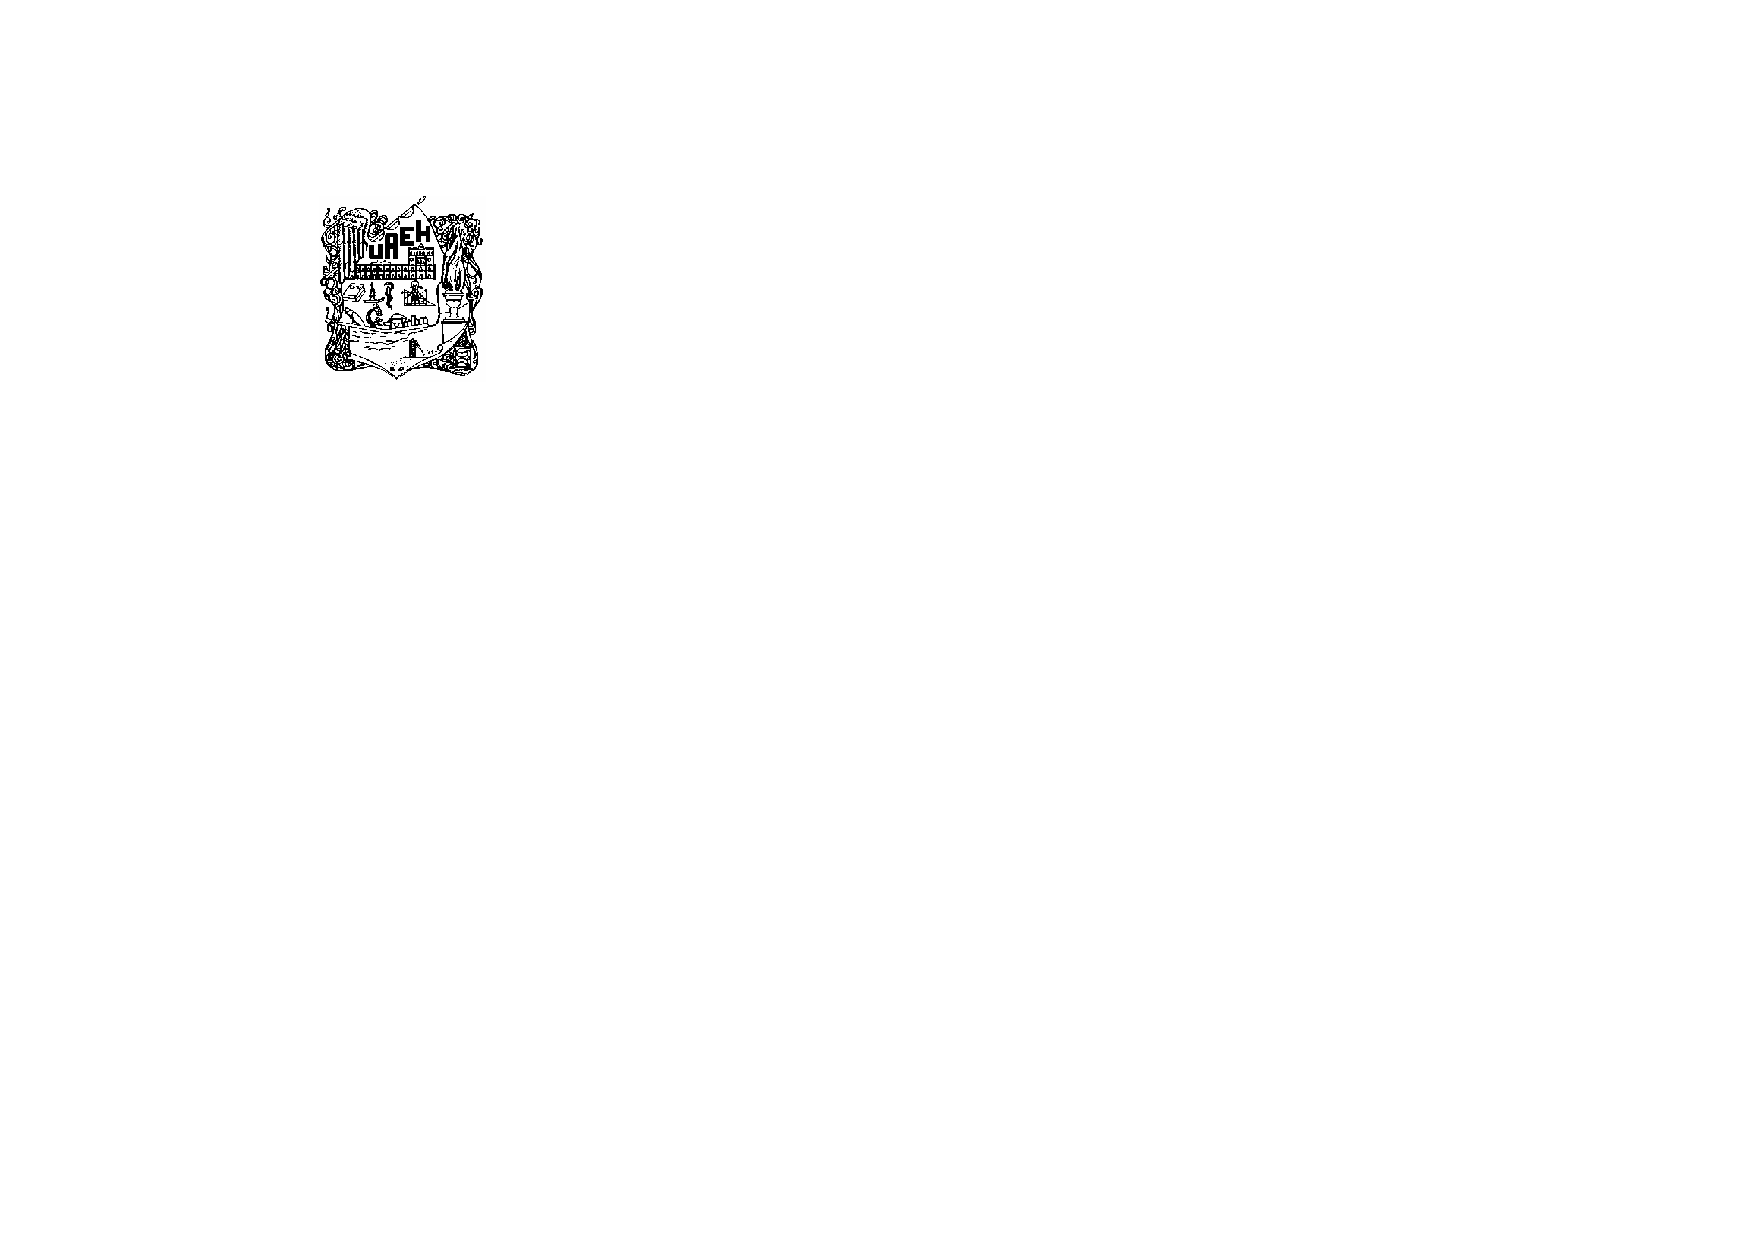
\includegraphics[scale=1.2,bb=55 20 0 0]{escudouaeh.pdf}

    \vspace*{\elespacio}

    \textsc{Universidad Autónoma del Estado de Hidalgo}

    \textsc{Instituto de Ciencias Básicas e Ingeniería}

    \textsc{Área Académica de Matemáticas y Física}

    \vspace*{\elespacio}

    {\Huge\bfseries Un enfoque computacional de representaciones de
      grupos en homologías\par}

    \vspace*{\elespacio}

    {\large Tesis que para obtener el título de}

    \vspace*{\elespacio}

    {\Large\textsc{Maestro en Matemáticas}}

    \vspace*{\elespacio}

    {\large presenta}

    \vspace*{\elespacio}

    {\Huge Manuel Campero Jurado}

    \vspace*{\elespacio}

    {\large bajo la dirección de}

    \bigskip

    {\Large Dr.~Rafael Villarroel Flores}

    \bigskip

    {Pachuca, Hidalgo. Octubre de 2018.}

    \vspace*{\fill}

  \end{center}
\end{titlepage}

\thispagestyle{empty}

\tableofcontents

\newpage

\begin{flushleft}
  {\bfseries\Large Resumen}
\end{flushleft}

En esta tesis se presentan los resultados de una librería realizada en
Python que permite calcular la descomposición en irreducibles del
$S_n$-módulo $\widetilde H_{k}(\Delta)$, donde $\Delta$ es un complejo
simplicial en el cual el grupo simétrico actúa permutando los
vértices, en particular este trabajo se interesa por complejos
simpliciales que provienen de un gráfica, específicamente de la
gráfica de líneas $G_n$ cuyo complejo de emparejamientos o matching
complex $M_n$ es bien conocido y del complejo simplicial $K(M_n)$ que
denota el complejo simplicial de la gráfica de clanes de $G_n$. Además
se busca encontrar una fórmula que descomponga al $S_n$-módulo
$\widetilde H_{k}(K(M_n))$ en submódulos irreducibles, así como Bouc
\cite{MR756517} lo realizó para $\widetilde H_{k}(M_n)$.

\vspace{2cm}

\begin{flushleft}
  {\bfseries\Large Abstract}
\end{flushleft}

In this thesis are presented the results of a library made in Python
that allows to calculate the decomposition into irreducible of the
$S_n$-module $\widetilde H_{k}(\Delta)$, where $\Delta$ is a
simplicial complex in which the symmetric group acts on the vertices
by permutation, In particular this work is interested in simplicial
complexes that come from a graph, specifically from the lines graph
$G_n$ whose matching complex $M_n$ is well known and from the
simplicial complex $K(M_n)$ that denotes the simplicial complex of the
clique graph of $G_n$. In addition, it is sought to find a formula
that decomposes the $S_n$-module $\widetilde H_{k}(K(M_n))$ into
irreducible submodules, as well as Bouc \cite{MR756517} did for
$\widetilde H_{k}(M_n)$.

 \newpage \thispagestyle{empty}
 
 \chapter*{Introducción}

 Una idea que generalmente aparece en la ciencia es que las grandes
 estructuras pueden ser comprendidas por medio de sus pedazo más
 pequeños. Lo mismo ocurre con la teoría de las
 representaciones. Algunas representaciones se construyen a partir de
 otras más pequeñas, mientras que otras son indivisibles. Esta es la
 distinción entre las representaciones reducibles y representaciones
 irreduccibles, algunas de las cuales estudiaremos en este
 trabajo. Sin embargo en este escenario primero es necesario
 determinar con precisión lo que significan estas piezas o
 sub-objetos.

 En la primera sección se presenta la acción de un grupo $G$ en un
 $\mathbb{C}$-espacio vectorial $V$, lo cual conduce definir un
 $G$-módulo. Mientras que una representación del grupo $G$ en el
 espacio vectorial $V$ es un homomorfismo de grupos $G \to GL(V)$,
 donde $GL(V)$ es el grupo de transformaciones lineales invertibles
 $V \to V$. Si el homomorfismo $G \to GL(V)$ es inyectivo, tenemos que
 $G$ es isomorfo a un subgrupo de $GL(V)$, es decir, hemos hallado una
 ``representación'' de los elementos $G$ como transformaciones
 lineales $V \to V$. Sin embargo las propiedades del homomorfismo
 $G \to GL(V)$ aún nos dan información de $G$ sin importar que no sea
 inyectivo. Se sabe que un $G$-módulo $V$ es equivalente a una
 representación $\phi \colon G \to GL(V)$.

 En el resto del primer capítulo diremos que una representación
 matricial $A$ es irreducible si no existe una matriz $P$ no singular tal
 que: $P^{-1}A(a)P$ es una matriz triangular inferior con ciertas
 características para todo $a \in G$. De ahí se formulan teoremas
 conocidos como el teorema de Maschke, Schur, entre otros cuyo análogos para
 $G$-módulos se escriben \textbf{encerrados en rectángulos}, ya que en
 ocasiones nos será útil la representación matricial y en otras
 ocasiones hablar en términos de $G$-módulos será más provechoso. Por
 último ser termina el capítulo introduciendo a los módulos de Specht
 $S^{\lambda}$, los cuales forman una lista completa de $S_n$-módulos
 irreducibles para $\lambda$ una partición de $n$ y las tablas de
 caracteres que son útiles para saber la multiplicidad de
 las representaciones irreducibles en un $G$-módulo.

 En el capítulo 2 sección \ref{asc} se definen conceptos como complejo
 simplicial abstracto $\Delta$, espacio de cadenas $C_{p}(\Delta)$ y
 el operador frontera $\partial_{p}$. En la sección \ref{hom_simpl} se
 presentan los conceptos de ciclos, fronteras y la función aumento que
 nos servirán para definir homología y homología reducida de un
 complejo simplicial. Finalmente la topología se asocia con un
 complejo simplicial $\Delta$ por medio de su realización geométrica
 $|\Delta|$.

En el capítulo $3$ se presentan conceptos básicos de gráficas así
como gráfica de líneas $G_n$ que surge a partir de gráficas completas
de $n$ vértices $K_n$ y gráfica de clanes $K(G_n)$ que se construyen
por medio de las gráficas $G_n$, cuyas homologías de sus complejo
simpliciales asociados y su descomposición en $S_n$-módulos
irreducibles es la principal inspiración de este trabajo. $K_n$, $G_n$
y $K(G_n)$ para $n = 5$ se presentan a continuación:

\begin{center}
  \begin{minipage}{0.3\linewidth}
    \centering
    \begin{tikzpicture}[rotate=90,scale=.7]
      \GraphInit[vstyle=Classic] 
      \SetUpVertex[MinSize=1pt]
      \SetVertexNoLabel 
      \grComplete[RA=2.3]{5}
    \end{tikzpicture}
  
    $K_{5}$
  \end{minipage}
  \bigskip

\begin{minipage}{0.33\linewidth}
  \centering
  \begin{tikzpicture}[rotate=90,scale=0.75]
    \newcommand{\aset}[2]{$\{#1,#2\}$} \GraphInit[vstyle=Classic]
    \SetUpVertex[MinSize=1pt] \SetVertexNoLabel
    \grPetersen[RA=2.8,RB=1.3]
  \end{tikzpicture}

  $G_{5}$
\end{minipage}\quad
\begin{minipage}{0.33\linewidth}
  \centering
  \begin{tikzpicture}[scale=.75]
    \newcommand{\aset}[2]{$\{#1,#2\}$} \GraphInit[vstyle=Classic]
    \SetUpVertex[MinSize=1pt] \SetVertexNoLabel
    \grEmptyCycle[RA=1,rotation=-90]{5}
    \grEmptyCycle[RA=1.8,prefix=w,rotation=-90]{5}
    \grCycle[RA=2.8,prefix=z,rotation=90]{5} \EdgeInGraphMod{a}{5}{2}
    \EdgeMod{a}{w}{5}{1} \EdgeMod{a}{w}{5}{-1} \EdgeMod{w}{z}{5}{2}
    \EdgeMod{w}{z}{5}{-2}
  \end{tikzpicture}
 
  $K(G_{5})$
\end{minipage}
\end{center} 


El capítulo $4$ se dan los conceptos de complejo de emparejamientos y
complejos simpliciales asociados a ciertas gráficas $K(G_n)$, se
enuncia el teorema de Bouc \cite{dong2002combinatorial}, y se exhiben
descomposiciones en $S_n$-módulos irreducibles de
$H_k(\Delta(K(G_7)))$ y $H_k(\Delta(K(G_8)))$ para algunos $k \geq 0$,
los cuales son los resultados obtenidos en la librería hecha en Python
que puede ser hallada en
\url{https://github.com/leunamCampero/Tesis/tree/master/Python} en el
archivo \textbf{representations.py} y que es una extensión de
\textbf{Sympy}.


El capítulo $6$ presenta la demostración del teorema de Bouc que puede
ser hallada en \cite{wachs2006poset}, y se especifica el camino que se
tiene planeado seguir para hallar una fórmula que permita la
descomposición en $S_n$-submódulos irreducibles de $H_k(K(M_n))$ para
todo $k,n \geq 0$.


\chapter{Representaciones de grupos}
\label{cha:Representaciones de grupos}

En este capítulo veremos las definiciones básicas de representaciones
de grupos. Nos basaremos principalmente en \cite{MR882540} y
\cite{sagan2001symmetric}.

\section{Definiciones básicas}
\label{sec:basicas}

\begin{definition}
  Sea $G$ un grupo y $X$ un conjunto no vacío. Una \textbf{acción de}
  $G$ \textbf{en} $X$ es una función $\ast \colon G \times X \to X$
  que cumple que para todo $x \in X$ y $g_1,g_2 \in G$:
  \begin{itemize}
  \item $1 \ast x = x.$
    \item $(g_1g_2) \ast x = g_1 \ast (g_2 \ast x)$.
  \end{itemize}
\end{definition}

Si se cumple lo anterior, $X$ es llamado un $G$-conjunto. Regularmente
escribimos $gx$ en vez de $g \ast x$.

\begin{definition}
  Si una acción de un grupo $G$ en un $\mathbb{C}$-espacio vectorial de
  dimensión finita $V$ cumple que para todo $g_1,g_2 \in G$, $v,w \in V$ y
  $\lambda \in \mathbb{C}$:
  \begin{itemize}
  \item $1v = v.$
  \item $(g_1g_2)v = g_1(g_2)v.$
  \item $g_1(v+w) = g_1v + g_2w.$
    \item $g_1(\lambda v) = \lambda (g_1v).$
    \end{itemize}
    Entonces se dirá que la acción de $G$-lineal y $V$ es un $G$\textbf{-módulo}.
\end{definition}

\begin{theorem}
  \label{acc_lin}
  Existe una biyección entre el conjunto de acciones lineales de un
  grupo $G$ en un $\mathbb{C}$-espacio vectorial $V$ y el conjunto de
  homomorfismos de $G$ en $GL(V)$.
\end{theorem}
\begin{proof}
Véase \cite{liebeck} teorema $4.4$, pg $40$.
\end{proof}
\begin{definition}
  \label{representation}
  Si $G$ es un grupo y $V$ un $\mathbb{C}$-espacio vectorial, una
  \textbf{representación} de $G$ en $V$ es un homomorfismo:
  $$\phi \colon G \to GL(V).$$
  La \textbf{dimensión} de la representación es
  definida como la dimensión del espacio vectorial $V$.
\end{definition}
Gracias al teorema \ref{acc_lin} analizar las representaciones de
  $G$ en un $\mathbb{C}$-espacio vectorial $V$ es equivalente a
  analizar $G$-módulos $V$. 
\begin{definition}
Sea $ \mathrm{GL}(n,\mathbb{C})$ el grupo de todas las matrices no
singulares $n\times n$ sobre el campo de los números complejos
$\mathbb{C}$ y sea $G$ un grupo. Una \textbf{representación (matricial)}
de $G$ se define como un homomorfismo:
\begin{equation*}
  A \colon a \mapsto \mathrm{GL}(n,\mathbb{C})
\end{equation*}
el cual por definición cumple que para todo $a, a_1,a_2 \in G$:
\begin{enumerate}
\item $A\left(a_1a_2\right)=A\left(a_1\right)A\left(a_2\right)$,
\item $A\left(1\right)=I_{n}$ (la matriz identidad $n\times n$),
\item $A\left(a^{-1}\right)=A\left(a\right)^{-1}$.
\end{enumerate}
es decir, observe que para todo $a \in G$, $A(a)$ es una matriz
$n \times n$ invertible con entradas en $\mathbb{C}$ asociada a
$\phi(a)$ que se obtiene fijando una base de $V$. El número $n$ se
llama \textbf{el grado} de la representación. Se dice que la
representación es \textbf{fiel} si $A$ es inyectiva.
\end{definition} 

\begin{example}
  \label{Ej6}
  La función que manda cada elemento de $G$ a $1
  \in \mathbb{C}$ es una representación de grado 1. Ésta es llamada la
  \textbf{representación unitaria} de $G$, y es denotada por $1_{G}$. 
\end{example}
\begin{example}
\label{ex_mod_per}
Sean $G$ un grupo, y $X$ el conjunto
$\{x_{1},x_{2},\ldots,x_{n}\}$. Luego consideremos
$\mathbb{C} X = \left \{ \lambda_1 x_{1} +\lambda_2 x_{2} + \cdots
  \lambda_n x_{n} : \lambda_{i} \in \mathbb{C} \right \}$, es decir,
el espacio vectorial generado por $X$ sobre $\mathbb{C}$.  La suma y
la multiplicación por escalar en $\mathbb{C} X$ está definida por:
  \begin{eqnarray*}
    (\lambda_{1}x_{1}+\lambda_{2}x_{2}+\cdots
    +\lambda_{n}x_{n})+(\lambda^{'}_{1}x_{1}+\lambda^{'}_{2}x_{2}+\cdots +\lambda^{'}_{n}x_{n})\\
    =(\lambda_{1}+\lambda^{'}_{1})x_{1}+(\lambda_{2}+\lambda^{'}_{2})x_{2}+\cdots
    +(\lambda_{n}+\lambda^{'}_{n})x_{n}
  \end{eqnarray*}
  y
  \begin{eqnarray*}
    c(\lambda_{1}x_{1}+\lambda_{2}x_{2}+\cdots +\lambda_{n}x_{n})=(c\lambda_{1})x_{1}+(c\lambda_{2})x_{2}+\cdots +(c\lambda_{n})x_{n},
  \end{eqnarray*}
  respectivamente. Sean $v\in \mathbb{C}X$, con
  $v=\lambda_{1}x_{1}+\lambda_{2}x_{2}+\cdots+\lambda_{n}x_{n}$ y $g\in G$, entonces la acción de $G$ en $\mathbb{C}X$ está dada por
  \begin{equation*}
    gv=g(\lambda_{1}x_{1}+\lambda_{2}x_{2}+\cdots +\lambda_{n}x_{n})=\lambda_{1}(gx_{1})+\lambda_{2}(gx_{2})+\cdots +\lambda_{n}(gx_{n}).
\end{equation*}
Luego $\mathbb{C}X$ es un $G$-módulo de dimensión $|X|$. 

Tomemos $G = S_3$ el grupo simétrico de $3$ elementos y
$X = \left \{ 1, 2, 3 \right \}$ y consideremos la base estándar
$\left \{ 1, 2, 3 \right \}$, entonces ya que para
$\pi = (123) \in S_3$, se tiene que $123(1) = 2$, $(123)2 = 3$ y
$123(3) = 1$ se sigue la matriz asociada a la base estándar es:
\begin{center}  
     $A(123)=\begin{pmatrix}
       0 & 0 & 1 \\
       1 & 0 & 0 \\
       0 & 1 & 0 \\
      \end{pmatrix}.$
\end{center}
Análogamente se encuentra que:
\begin{center}  
     $A(1)=\begin{pmatrix}
       1 & 0 & 0 \\
       0 & 1 & 0 \\
       0 & 0 & 1 \\
      \end{pmatrix}$
\end{center}
y
\begin{center}  
     $A(12)=\begin{pmatrix}
       0 & 1 & 0 \\
       1 & 0 & 0 \\
       0 & 0 & 1 \\
      \end{pmatrix}.$
\end{center}
\end{example}
Más adelante se explicará porqué para nuestros fines no es necesario
calcular $A(g)$ para $g \in \left \{ (13),(23),(132) \right \}$ una
vez que se tiene lo anterior.
\begin{example}
  \label{Ej5}
  Dadas una representación $A$ y una matriz no singular $P$, la regla:
  \begin{equation*}
    a \mapsto P^{-1}A\left(a\right)P
  \end{equation*}  
  induce una representación de $G$.

  Sean $A$ y $B$ representaciones de $G$. Si existe una
  matriz no singular $P$ tal que para todo $a \in G$:
  \begin{equation*}
    B\left(a\right)= P^{-1}A\left(a\right)P,
  \end{equation*}
  entonces se dirá que $A$ y $B$ son
  \textbf{equivalentes}. Representaciones equivalentes se denotan como
  $A \sim B$. La relación $\sim$ define una clase de equivalencia de
  representaciones de $G$.
\end{example}

\begin{example}
  \label{Ej3}
  Sea $S_{n}$ el grupo simétrico de grado
  $n$. Para un elemento
  \begin{equation}
    \label{eq:1}
    \sigma =
    \begin{pmatrix}
      1 & 2 & \cdots  & n\\
      s_{1} & s_{2} & \cdots & s_{n}
    \end{pmatrix} 
    \in S_{n},
  \end{equation}
  y sea
  \begin{equation*}
    \alpha_{ij}\left(\sigma\right) = \left\{
      \begin{array}{ll}
        1      & \mathrm{si\ } j = s_{i}, \\
        0      & \mathrm{otro\ caso,\ } 
      \end{array}
    \right.
  \end{equation*}
  entonces definimos $A\left(\sigma\right)$ como la matriz cuyo
  $i$-ésimo renglón es $\left(0,...,0,1,0,...,0\right)$ con 1 en el
  $s_{i}$-ésimo lugar, por lo cual para $\left(i,j=1,2,...,n\right)$
  se tiene:
  \begin{equation*}
    A\left(\sigma\right) = \left(\alpha_{ij}\left(\sigma\right)\right).
  \end{equation*}
  La regla $\sigma \mapsto A\left(\sigma\right)$ es una representación
  fiel de $S_{n}$.
\end{example}


\begin{example}
  \label{Ej4}
  Sea $G$ un grupo finito cuyos elementos son $a_{1},a_{2},...,a_{n}$
  y sea $S^{G}$ el grupo simétrico de $G$. La función bajo la cual
  cada elemento $a \in G$ es llevado a la permutación \ref{eq:6} es un
  homomorfismo inyectivo de $G$ en $S^{G}$.
  \begin{equation}
    \label{eq:6}
    \begin{pmatrix}
      a_{1} & a_{2} & \cdots  & a_{n}\\
      a_{1}a & a_{2}a & \cdots & a_{n}a
    \end{pmatrix} 
    \in S_{n}^{G}.
  \end{equation}
  Sea
  \begin{equation*}
    \alpha_{ij} (a) = \left\{
      \begin{array}{ll}
        1      & \mathrm{si\ } a_{i}a = a_{j}, \\
        0      & \mathrm{otro\ caso,\ }
      \end{array}
    \right. 
  \end{equation*}
  entonces a \ref{eq:6} se le asocia la matriz. 
  \begin{equation*}
    A(a)=\big(\alpha_{ij}(a)\big).
  \end{equation*} 
  Entonces la regla $a \mapsto A\left(\sigma\right)$ se convierte en
  una representación fiel de $G$. A ésta se le llama \textbf{representación
  regular derecha} de $G$. Sea $\delta{(a)}$ de la siguiente manera:
  \begin{equation*}
    \delta{(a)} = \left\{
      \begin{array}{ll}
        1      & \mathrm{si\ } a = 1, \\
        0      & \mathrm{otro\ caso,\ } 
      \end{array}
    \right.
  \end{equation*}
  entonces formamos la matriz \ref{eq:7}, y se observa que si
  $a \neq 1$ cada elemento sobre la diagonal es cero.
  \begin{equation}
    \label{eq:7}
    A\left(a\right) = 
    \begin{pmatrix}
      \delta\left(a_{1}aa_{1}^{-1}\right) & \delta\left(a_{1}aa_{2}^{-1}\right) & \cdots  & \delta\left(a_{1}aa_{n}^{-1}\right)\\
      \delta\left(a_{2}aa_{1}^{-1}\right) & \delta\left(a_{2}aa_{2}^{-1}\right) & \cdots  & \delta\left(a_{2}aa_{n}^{-1}\right)\\ 
      \vdots & \vdots & \ddots & \vdots\\
      \delta\left(a_{n}aa_{1}^{-1}\right) & \delta\left(a_{n}aa_{2}^{-1}\right) & \cdots  & \delta\left(a_{n}aa_{n}^{-1}\right)
    \end{pmatrix}
    .
  \end{equation}

  La \textbf{representación regular izquierda} de $G$ se define
  análogamente usando el siguiente homomorfismo:
  \begin{equation*}
    a \mapsto
    \begin{pmatrix}
      a_{1} & a_{2} & \cdots  & a_{n}\\ 
      aa_{1} & aa_{2} & \cdots & aa_{n}
    \end{pmatrix}.
  \end{equation*}
  lo cual significa que
  \begin{equation}
    \label{eq:8}
    A\left(a\right) = 
    \begin{pmatrix}
      \delta\left(a_{1}^{-1}aa_{1}\right) & \delta\left(a_{1}^{-1}aa_{2}\right) & \cdots  & \delta\left(a_{1}^{-1}aa_{n}\right)\\
      \delta\left(a_{2}^{-1}aa_{1}\right) & \delta\left(a_{2}^{-1}aa_{2}\right) & \cdots  & \delta\left(a_{2}^{-1}aa_{n}\right)\\ 
      \vdots & \vdots & \ddots & \vdots\\
      \delta\left(a_{n}^{-1}aa_{1}\right) & \delta\left(a_{n}^{-1}aa_{2}\right) & \cdots  & \delta\left(a_{n}^{-1}aa_{n}\right)
    \end{pmatrix}
    .
  \end{equation}
\end{example}

Entonces se tiene que si $\phi \colon a \mapsto \phi\left(a\right)$ es
un homomorfismo de $G$ en~$S_{n}$ (es decir, una representación
permutación de $G$). Expresando la permutación $\phi\left(a\right)$
por la matriz $A\left(a\right)$ como en el ejemplo \ref{Ej3}, se
obtiene una representación matricial.

Ahora sean $A$, $B$ y $C$ representaciones de grado $n$,
$r \geq 1$ y $s \geq 1$ respectivamente, con $r+s=n$. Entonces se dice
que $A$ es \textbf{reducible} si para todo $a \in G$ hay una matriz no
singular $P$ tal que:

\begin{equation*}
  P^{-1}A\left(a\right)P=
  \begin{pmatrix}
    B\left(a\right) & 0 \\
    D\left(a\right) & C\left(a\right)
  \end{pmatrix}. 
\end{equation*}  
Y además se observa que las representaciones
\begin{equation*}
  A_{1}\left(a\right)=
  \begin{pmatrix}
    B\left(a\right) & 0 \\
    D\left(a\right) & C\left(a\right)
  \end{pmatrix}
\end{equation*}
y
\begin{equation*} 
   A_{2}\left(a\right)=
  \begin{pmatrix}
    C\left(a\right) & D\left(a\right) \\
    0 & B\left(a\right)
  \end{pmatrix}
\end{equation*}
son equivalentes, porque para $I_{r}$ y $I_{s}$ matrices identidad de
grado $r$ y $s$ respectivamente y para $Q$ de la siguiente manera:
\begin{equation*}
  Q=
  \begin{pmatrix}
    0 & I_{r} \\ 
    I_{s} & 0
  \end{pmatrix},
\end{equation*}
se tiene que $Q^{-1}A_{1}\left(a\right)Q=A_{2}\left(a\right)$.


Si $A$ no es reducible, se dice que $A$ es \textbf{irreducible}. En el ejemplo
\ref{Ej3}, las reglas de correspondencia $a \mapsto B\left(a\right)$ y
$a \mapsto C\left(a\right)$ se convierten en representaciones de
grado~$r$,~$s$, respectivamente.

\begin{mdframed}
  Análogamente si $V$ es un $G$-módulo. $W$ es llamado $G$-submódulo o
  submódulo de $V$ si $W$ es un subespacio invariante bajo la acción
  de $G$, es decir que $gw \in W$ para todo $w \in W$ y $g \in G$, tal
  que $W$ es un $G$-módulo en sí mismo bajo la acción de $G$. Se
  escribirá $W \leq V$ si $W$ es un submódulo de $V$. Se dirá que $V$
  un $G$-módulo no trivial es \textbf{irreducible} si sus únicos submódulos son
  el submódulo trivial $0$ y $V$ mismo. 
\end{mdframed}
 

Sean $A$ y $B$ representaciones de $G$, con grados $n$, $m$,
respectivamente, la función dada por:
\begin{equation*}
  a\mapsto
  \begin{pmatrix}
    A\left(a\right) & 0 \\ 
    0 & B\left(a\right)
  \end{pmatrix}, 
\end{equation*}
se convierte en una representación de $G$ de grado $n+m$. Esta
representación es llamada la \textbf{suma directa} de $A$ y
$B$, y es denotada por $A \oplus B$.

Una representación $A\left(a\right)$ de $G$ se dice \textbf{completamente
reducible} si $A$ es equivalente a la suma directa de algunas
representaciones irreducibles, es decir, si existe una matriz no singular
$P$, tal que

\begin{equation*}
 P^{-1}A\left(a\right)P=
 \begin{pmatrix}
   F_{1}(a) & & & 0\\
   & F_{2}(a) & & \\
   & & \ddots & \\
   0 & & & F_{r}(a),
 \end{pmatrix}
\end{equation*}
donde cada $F_{i}\left(a\right)$ con $i=1,2,...,r$ es una
representación irreducible de $G$.

\begin{mdframed}
  Similarmente si $U,V$ son dos espacios vectoriales. Entonces la
  \textbf{suma directa externa} de $U$ y $V$ es el conjunto
  $U \times V = \left \{ (u,v) \colon u \in U, v \in V \right \}$ con
  las siguientes operaciones:
  \begin{equation}
    \label{eq:94}
    \begin{split}
(u,v)+(u_1+v_1) & = (u+u_1,v+v_1), \\
 & k(u,v) = (ku,kv),
\end{split}
  \end{equation}
  con $u, u_1 \in U$ y $k \in \mathbb{C}$. Con estas operaciones
  $U \times V$ es un espacio vectorial que se denotará por
  $U \otimes V$.  Por lo cual, dados $U$ y $W$ $G$-módulos, se tiene
  que $U \times W$ también es un $G$-módulo con acción
  $a(v,w) = (av,aw)$ para $a \in G$. Lo anterior puede ser extendido a
  una cantidad finita de $G$-módulos.
\end{mdframed}
\section{Representaciones por matrices unitarias}
\label{sec:munitarias}

Una representación $A$ de $G$ se dice \textbf{unitaria} si $A\left(a\right)$ es
una matriz unitaria para todo $a \in G$, lo cual significa que
$A^{*}A\left(a\right)=I$. Aquí $A^{*}$ denota la transpuesta de
$\overline{A}=\left(\alpha_{ij}\right)$, donde
$A=\left(\alpha_{ij}\right)$, y $\overline{\left(\alpha_{ij}\right)}$
es el complejo conjugado de $\left(\alpha_{ij}\right)$. Se pretende
mostrar que cada representación de un grupo finito es equivalente a
una representación unitaria y es completamente reducible.

Una matriz se dice hermitiana si $A^{*}=A$, y positiva definida si
$x^{*}Ax>0$ para todo vector columna $x$ (distinto de cero).

\begin{lemma}
  \label{l2_1}
  Para cualquier matriz no singular $A$, $A^{*}A$ es una matriz
  hermitiana definida positiva. La suma de matrices hermitianas
  definidas positivas, también es hermitiana y definida positiva.

\end{lemma}

\begin{lemma}
  \label{l2_2}
   Para cualquier matriz hermitiana definida positiva
$A$, existe una matriz triangular superior no singular $C$ tal que
$C^{*}AC=\mathrm{I}$.
\end{lemma}

\begin{proof}
  Sea $A\left(\alpha_{ij}\right)=(\alpha_{ij})$, entonces para
  $\left(i,j=1,2,...,n\right)$ se tiene que
  $\alpha_{ji}=\overline{\alpha_{ij}}$ y además
  $\left(\alpha_{ii}\right)>0$. Por ello $A$ tiene la forma:
  \begin{equation}
    \label{eq:2}
     A=
     \begin{pmatrix}
    \alpha & a \\ 
    a^{*} & \mathrm{B},
  \end{pmatrix}
  \end{equation} 

  donde $\alpha=\alpha_{11}>0$,
  $ a= \left(\alpha_{12},\alpha_{13},...,\alpha_{1n} \right) $,
  $ \mathrm{B}=\left(\alpha_{ij}\right)$,
  $ \left(i,j=2,...,n\right) $. Por otro lado, sea
\begin{equation}
  \label{eq:3}
  C_{1}=
  \begin{pmatrix}
    \frac{1}{\sqrt{\alpha}} & -\frac{a}{\alpha} \\ 
    0 & \mathrm{I}
  \end{pmatrix}
\end{equation}
entonces, 
\begin{equation}
   \label{eq:4}
  C_{1}^{*}AC_{1} =
  \begin{pmatrix}
    1 & 0 \\ 
    0 & -\frac{1}{\alpha}a^{*}a+\mathrm{B}
  \end{pmatrix}
\end{equation}  
y $-\frac{1}{\alpha}a^{*}a+\mathrm{B}$ es una matriz hermitiana
definida positiva. Y la prueba se sigue usando inducción el grado de
$A$ veces.
\end{proof}

\begin{theorem}
  \label{t2_3}
  Sea $G$ un grupo finito. Para una representación $F$ de $G$,
  entonces existe una matriz triangular superior no singular $C$,
  tal que $C^{-1}F\left(a\right)C$ es una matriz unitaria para todo
  $a \in G$.
\end{theorem}

\begin{proof}
  Sea
  \begin{equation*}
    A=\sum_{b \in G} F \left(b\right)^{*}F\left(b\right).
  \end{equation*}
  Entonces $A$ es una matriz hermitiana definida positiva por el Lema
  2.1. Entonces existe una matriz triangular no singular $C$, tal que
  \begin{equation*}
    C^{*}AC= I
  \end{equation*}
  y por ello
  \begin{equation}
    \label{eq:9}
    A=(C^{*})^{-1}C^{-1}.
  \end{equation}
  Ya que
  \begin{equation}
    \label{eq:10}
    F\left(a\right)^{*} AF\left(a\right)=\sum_{b \in G} F\left(ba\right)^{*} F\left(ba\right)=A,
  \end{equation}
  se obtiene
  \begin{equation}
    \label{eq:11}
    F\left(a\right)^{*}(C^{*})^{-1}C^{-1}F\left(a\right)=(C^{*})^{-1}C^{-1},
  \end{equation}
  es decir
  \begin{equation}
    \label{eq:12}
    (C^{-1}F(a)C)^{*}(C^{-1}F(a)C)=I
  \end{equation}
  y $C^{-1}F(a)C$ es una matriz unitaria.
\end{proof}
\begin{theorem}
  \label{t2_4}
  Una representación de un grupo finito es
  completamente reducible.
\end{theorem}
\begin{proof}
  Sea $A$ una representación de un grupo finito de $G$ y sea $A(a)$
  descompuesta como
  \begin{equation}
    \label{eq:13}
        A(a)=
    \begin{pmatrix}
      A_{1}(a) & * \\ 
      0 & A_{2}(a)
    \end{pmatrix}.
  \end{equation}
  Por el teorema anterior, existe una matriz triangular no superior
  $C$ tal que $C^{-1}A(a)C$ es una matriz unitaria. Sea
  $U(a)=C^{-1}A(a)C$. Como $C$ es una matriz triangular superior,
  $U(a)$ se descompone como:
  \begin{equation}
    \label{eq:14}
    U(a)=
    \begin{pmatrix}
      U_{1}(a) & V(a) \\ 
      0 & U_{2}(a).
    \end{pmatrix}
  \end{equation}  
  Y ya que $U(a)^{*}=U(a)^{-1}=U(a^{-1})$, se obtiene
  \begin{equation}
    \label{eq:15}
    \begin{pmatrix}
      \overline{U_{1}(a)}^{t} & 0 \\ 
      \overline{V(a)}^{t} & \overline{U_{2}(a)}^{t}
    \end{pmatrix}
    =
    \begin{pmatrix}
      U_{1}(a^{-1}) & V(a^{-1}) \\ 
      0 & U_{2}(a^{-1}),
    \end{pmatrix}
  \end{equation}
  luego $V(a)=0$.
\end{proof}

\begin{mdframed}
  (\textit{Teorema de Maschke}) Sea $G$ un grupo finito y $V$ un
  $G$-módulo. Entonces $V$ es \textbf{completamente reducible}, es
  decir:
  \begin{equation}
    \label{eq:95}
    V \cong m_1W^{(1)} \oplus m_2W^{(2)} \oplus  \cdots \oplus m_kW^{(k)}, 
  \end{equation}
  donde $W^{(i)}$ y $W^{(j)}$ son $G$-módulos irreducibles de $V$ no
  isomorfos de $V$ para $i \neq j$ y $m_i$ es la cantidad de $W^{(i)}$
  (multiplicidad de $W^{(i)}$ en $V$.)
\end{mdframed}
\section{Lema de Schur}
\label{sec:schur}

\begin{lemma}[\textit{Lema de Schur}]
  \label{l3_1}
  Sean $A$ y $B$ representaciones
  irreducibles de un grupo $G$ con grados $m$ y $n$ respectivamente. Sea
  $P$ una matriz de $m \times n$ con la propiedad de que $A(a)P=PB(a)$, para
  todo $a \in G$.  entonces:
  \begin{enumerate}
  \item $P=0$
  \item $m=n$ y $P$ es no singular.
  \end{enumerate}
\end{lemma}

\begin{proof}
  Asumimos $P \neq 0$. Y se quiere mostrar la segunda
  condición. Supongamos que $m \neq n$, o $m=n$ y $P$ es
  singular. Entonces existe $Q \in \mathrm{GL}(m,\mathbb{C})$ y
  $R \in \mathrm{GL}(n,\mathbb{C})$, tal que
  \begin{equation}
    \label{eq:16}
    QPR=
    \begin{pmatrix}
      I_{r} & 0 \\ 
      0 & 0,
    \end{pmatrix} 
  \end{equation}
  donde $I_{r}$ es la matriz identidad de grado $r$. con
  $r<$max$\left\{ m,n \right\}$. Como
  $QA(a)Q^{-1}(QPR) = QPR(R^{-1}B(a)R)$, y se obtiene
  \begin{equation}
    \label{eq:17}
    \begin{pmatrix}
      A_{11} & 0 \\ 
      A_{21} & 0
    \end{pmatrix}
    =
    \begin{pmatrix}
      B_{11} & B_{12} \\ 
      0 & 0
    \end{pmatrix},
  \end{equation}
  donde
  \begin{equation}
    \label{eq:18}
    QA(a)A^{-1}=
    \begin{pmatrix}
      A_{11} & A_{12} \\ 
      A_{21} & A_{22}
    \end{pmatrix} 
  \end{equation}  
  con $A_{11}$ una matriz cuadrada de grado $r$. Y
  \begin{equation}
    \label{eq:19}
    R^{-1}B(a)R=
    \begin{pmatrix}
      B_{11} & B_{12} \\ 
      B_{21} & B_{22},
    \end{pmatrix}
  \end{equation}
  con $B_{11}$ una matriz cuadrada de grado $r$. Por lo tanto
  $A_{21}=0$ si $r<m$ y $B_{12}$ si $r<n$. De cualquier manera
  $A$ o $B$ es reducible, lo cual es una
  contradicción.
\end{proof}

\begin{mdframed}
  Si $V$ y $W$ son $G$-módulos, $f \colon V \to W$ un morfismo de
  $G$-módulos, $S \leq V$ con $S$ irreducible, entonces $f \cong S$ o
  $f(S) = 0$.
\end{mdframed}
\begin{theorem}
  \label{t3_2}
  Sea $A$ una representación irreducible de un grupo $G$. Sea $P$ una
  matriz con la propiedad $A(a)P=PA(a)$ para todo $a \in G$. Entonces
  $P=\lambda I$, para algún $\lambda \in \mathbb{C}$.
\end{theorem}
\begin{proof}
  Sea $\lambda$ un valor propio de $P$. Entonces
  $\det(\lambda I - P)=0$, y además para todo $a \in G$
  \begin{equation}
    \label{eq:20}
    A(a)(\lambda I - P)=(\lambda I - P)A(a)
  \end{equation}
  Entonces por el Lema de Schur,
  \begin{equation}
    \label{eq:21}
    \lambda I-P=0
  \end{equation}
\end{proof}

\begin{theorem}
  \label{t3_3}
  Sea $G$ un grupo abeliano. Entonces cada
representación irreducible de $G$ es de grado 1.
\end{theorem}

\begin{proof}
  Sea $A$ una representación irreducible de $G$. Como $A(a)$ conmuta
  con $A(b)$, el teorema \ref{t3_2} nos dice que $A(a)=\lambda(a) I$
  para algún $\lambda(a) \in \mathbb{C}$. Entonces $A$ es irreducible,
  y su grado debe ser $1$.
\end{proof}

\section{Relación ortogonal de caracteres}
\label{sec:roc}
Desde aquí en adelante se asumirá que estamos trabajando con grupos
finitos.

\textbf{Caracteres}\\
Para una matriz cuadrada $A=(\alpha_{ij})$ de grado
$n$, $\tr A$ denota la \textbf{traza} de $A$, es decir
\begin{itemize}
  \item $\tr A= \alpha_{11}+ \alpha_{22} + \cdots + \alpha_{nn}$.
  \end{itemize}

Cálculos directos muestran el siguiente lema

\begin{lemma}
   \label{l4_1}
  \begin{enumerate} Para alguna matriz no singular $P$, se sigue que:
  \item $\tr (AB)=\tr (BA) $.
  \item $\tr (P^{-1}AP)=\tr A$.
  \end{enumerate}
\end{lemma}

Para una representación $A$ de un grupo $G$, sea $\tr
A(a)=\chi(a)$. Entonces~$\chi$ es una función que toma valores en
$\mathbb{C}$ y es llamada el \textbf{carácter} de~$A$. Obviamente,
$\chi(1)$ es igual al grado de $A$. Caracteres de representaciones
irreducibles son llamados \textbf{caracteres irreducibles}. Y por el
lema \ref{l4_1}(2), se tiene lo siguiente:

\begin{lemma}
  \label{l4_2}
  Representaciones equivalentes de un grupo tienen el mismo carácter.
\end{lemma}
\begin{proof}
  La prueba se sigue de la segunda parte del lema \ref{l4_1} y la
  definición de representación equivalente.
\end{proof}
Como $A(x^{-1}ax)=A(x)^{-1}A(a)A(x)$, se sigue que
$ \chi(x^{-1}ax)=\chi(a)$. Así~$\chi$ toma el mismo valor en una clase
de conjugación de $G$. Tal función es llamada \textbf{función de clase}.

\subsection{La primera relación ortogonal de caracteres.}
\label{subsec:roc1}
Sea $G$ un grupo de orden $g$. Sean $A=(\alpha_{ij}(a))$ y
$B=(\beta_{ij}(a))$ representaciones irreducibles de $G$ con grado
$m,n$, respectivamente. Para una matriz arbitraria $U=(\gamma_{ij})$,
de $m \times n$, se tiene

\begin{equation}
  \label{eq:22}
  V=\sum_{x \in G} A(x)UB(x^{-1}).  
\end{equation}
Entonces
\begin{equation}
  \label{eq:23}
  \begin{aligned}
    A(a)V &=\sum_{x \in G} A(ax)UB(x^{-1})\\
    &=\sum_{y \in G} A(y)UB(y^{-1}a) \qquad (y=ax)\\
    &=\sum_{y \in G} A(y)UB(y^{-1})B(a).
  \end{aligned}
\end{equation}
Como $y$ varía sobre $G$ conforme $x$ lo hace, se tiene
\begin{equation}
  \label{eq:24}
  A(a)V=VB(a).
\end{equation} 
Asumimos que $A$ y $B$ no son equivalentes. Entonces $V=0$ por el Lema
de Schur. La entrada $(i,j)$ de $V$ es:
\begin{equation}
  \label{eq:25}
  \sum_{x \in G} \sum_{u,v} \alpha_{iu}(x) \gamma_{uv} \beta_{vj}(x^{-1}) = 0.
\end{equation}
En particular, para algún par de $u$,$v$ sea $\gamma_{uv}=1$ y para
cualquier otro caso~$\gamma_{\rho \sigma}=0$. Lo cual conduce a
\begin{equation}
  \label{eq:26}
  \sum_{x \in G} \alpha_{iu}(x) \beta_{vj}(x^{-1}) = 0.
\end{equation}
Ahora, asumimos que $A=B$. Entonces para algún
$\lambda \in \mathbb{C}$, $V=\lambda I$ por el teorema \ref{t3_2}. La
entrada $(i,j)$ de $V$ es:
\begin{equation}
  \label{eq:27}
   \sum_{x \in G} \sum_{u,v} \alpha_{iu}(x) \gamma_{uv} \alpha_{vj}(x^{-1}) = \delta_{ij}\lambda,
\end{equation}
donde $\delta_{ii}=1$, $\delta_{ij}=0$ ($i \neq j$). Tomando la traza de
\begin{equation}
  \label{eq:28}
  \sum_{x \in G} A(x)UA(x^{-1}) = \lambda I,
\end{equation}
y se obtiene
\begin{equation}
  \label{eq:29}
  g(\gamma_{11}+\gamma_{22}+ \cdots +\gamma_{nn})=n \lambda,
\end{equation}
donde $n$ es el grado de $A$, y $g$ es la cardinalidad de $G$, de lo cual se sigue:
\begin{equation}
  \label{eq:30}
  \lambda=\frac{g}{n}(\gamma_{11}+\gamma_{22}+ \cdots + \gamma_{nn}).
\end{equation}
Ahora, para algún par de $u$,$v$ sea $\gamma_{uv}=1$ y en otro caso~$\gamma_{\rho \sigma}=0$. Entonces
\begin{equation}
  \label{eq:31}
  \sum_{x \in G} \alpha_{iu}(x) \alpha_{vj}(x^{-1}) = \delta_{ij} \delta_{uv}\frac{g}{n}.
\end{equation}
Lo cual nos conduce al siguiente teorema.
\begin{theorem}
  \label{t4_3}
  Sea $G$ un grupo de orden $g$.
  \begin{enumerate}
  \item Sea $A(a)=(\alpha_{ij}(a))$ una representación irreducible de
    $G$ con grado $n$. Entonces
    \begin{equation*}
      \sum_{x \in G} \alpha_{iu}(x) \alpha_{vj}(x^{-1})
      = \delta_{ij} \delta_{uv}\frac{g}{n}.
    \end{equation*}
  \item Sea $ B(a)=(\beta_{ij}(a))$ una representación irreducible, la
    cual no es equivalente a $A$, entonces
    \begin{equation*}
      \sum_{x \in G} \alpha_{iu}(x) \beta_{vj}(x^{-1}) =0.
    \end{equation*}
    \end{enumerate}
\end{theorem}
Sean $\chi$, $\chi^{'}$ los caracteres de $A$, $B$. Por el teorema
anterior, poniendo a~$u=i$, $v=j$ y tomando la suma sobre $i$,$j$, se
obtiene lo siguiente:
\begin{theorem}[La primera relación de ortogonalidad de caracteres]
  \label{t4_4}
  Sea $G$ un grupo de orden $g$.
  \begin{enumerate}
  \item Sea $\chi$ un carácter irreducible de $G$, entonces 
  \begin{equation*}
    \sum_{x \in G} \chi(x) \chi(x^{-1}) = g.
  \end{equation*}
  \item Sea $\chi$, $\chi^{'}$ caracteres de representaciones
    irreducibles no equivalentes de $G$, entonces
  \begin{equation*}
    \sum_{x \in G} \chi(x) \chi^{'}(x^{-1}) = 0.
  \end{equation*}
  \end{enumerate}
\end{theorem}
Se observa que $\chi(a^{-1})=\overline{\chi(a)}$ para todo $a \in G$,
porque el teorema \ref{t2_3} dice que $A$ es equivalente a una
representación unitaria $U$, y por lo tanto
\begin{equation}
  \label{eq:34}
  \chi(a^{-1})=\tr U(a^{-1})=\tr U(a)^{-1}=\tr U(a)^{*} = \overline{\chi(a)}  
\end{equation}
Sean $F_{1}, F_{2}, \ldots$ representantes de las clases de
equivalencia de las representaciones irreducibles de un grupo $G$ y
para $i=1,2, \ldots$ sea $\chi_{i}$ el correspondiente carácter
de $F_{i}$.  Sean $C_{1}$, $C_{2}$,...,$C_{k}$ las
clases de conjugación de $G$ con~$|C_{\alpha}|=h_{\alpha}$
para $\alpha=1, 2, 3,...,k$ y sean $a_{1}$, $a_{2}$,\ldots,$a_{k}$ los
representantes de las clases de conjugación. Como los caracteres son
funciones de clases, el teorema \ref{t4_4} se reescribe como sigue
\begin{theorem}
  \label{t4_4p}
  \begin{equation}
    \label{eq:32}
    \sum_{\alpha=1}^{k} h_{\alpha} \chi_{i}(a_{\alpha}) \overline{\chi_{j}(a_{\alpha})} = \delta_{ij}g.
  \end{equation}
\end{theorem}
Para funciones $\varphi$, $\psi$ que toman valores en $\mathbb{C}$ en
un grupo $G$ de orden $g$, se define el \textbf{producto interno}
$(\varphi,\psi)_{G}$ de la siguiente manera
\begin{equation*}
(\varphi,\psi)_{G} = \frac{1}{g} \sum_{x \in G} \varphi(x) \psi(x^{-1}).
\end{equation*}
Cuando sea claro que se está hablando del grupo $G$, se escribirá
$(\varphi,\psi)$ en lugar de $(\varphi,\psi)_{G}$. Claramente el
producto interno cumple las siguientes propiedades
\begin{equation}
  \label{eq:33}
    \begin{aligned}
    (\varphi,\psi) &= (\psi,\varphi), \\
    (\varphi_{1}+\varphi_{2},\psi) &= (\varphi_{1},\psi)+(\varphi_{2},\psi), \\
    (\varphi,\psi_{1}+\psi_{2}) &= (\varphi,\psi_{1})+(\varphi,\psi_{2}), \\
    (\lambda \varphi,\psi) &= (\psi,\lambda \varphi)=\lambda (\varphi,\psi).
  \end{aligned}
\end{equation}
Con esta notación la primera relación de ortogonalidad de caracteres
es expresada como sigue:

\begin{theorem}
  \label{t4_4pp}
  Sean $\chi_{1}$, $\chi_{2}$,... los caracteres de caracteres de
  representaciones no equivalentes de un grupo $G$. Entonces
  \begin{equation*}
    (\chi_{i},\chi_{j})=\delta_{ij}.
  \end{equation*} 
\end{theorem}
\subsection{Multiplicidad de representaciones irreducibles.}
\label{subsec:mri}
 Sea $A$ una representación de un grupo $G$. Como $A$ es completamente
reducible, entonces por el teorema \ref{t2_3}, $A$ es equivalente a
\begin{equation}
  \label{eq:35}
  \begin{aligned}
    \begin{pmatrix}
      F_{1} & & & & & & 0\\ 
      & \ddots & & & & & \\
      & & F_{1} & & & & \\
      & & & F_{2} & & & \\
      & & & & \ddots & & \\
      & & & & & F_{2} & \\
      0 & & & & & & \ddots
    \end{pmatrix},
  \end{aligned}
\end{equation}
donde $F_{1}, F_{2}, \ldots$ son representaciones no equivalentes. Y
$F_{i}$ se repite $m_{i}$~-veces en \ref{eq:35}, a este número se le
conoce como la \textbf{multiplicidad} de $F_{i}$ en $A$, y además si $m_{i}=0$
entonces $F_{i}$ no aparece, y se escribe
\begin{equation}
  \label{eq:36}
  A \sim m_{1} F_{1}+ m_{2} F_{2}+ \cdots .
\end{equation}
Sea $\chi$ el carácter de $A$ y $\chi_{i}$ el carácter de $F_{i}$
para $i = 1, 2, ...$. Entonces
\begin{equation}
  \label{eq:37}
  \chi =m_{1} \chi_{1}+ m_{2} \chi_{2}+ \cdots .
\end{equation}
Si $m_{i} \neq 0$, $F_{i}$ y $\chi_{i}$ son llamados \textbf{componentes
irreducibles} de $A$ y $\chi$ respectivamente.

\begin{theorem}
  \label{t4_5}
  Sea $G$ un grupo y sea $\chi$ el carácter de una
  representación de $G$. Sea $m_{i}$ la multiplicidad de un carácter
  irreducible $\chi_{i}$ en $\chi$. Entonces
  \begin{equation*}
    m_{i} = (\chi,\chi_{i}) = \frac{1}{g} \sum_{x \in G} \chi(x) \overline{\chi_{i}(x)}
  \end{equation*}

\end{theorem}
\begin{proof}
  Sea $$\chi=\sum_{j} m_{j} \chi_{j}$$ la suma de caracteres
  irreducibles con $m_{j}$ la multiplicidad de $\chi_{j}$. Entonces
  \begin{equation}
    \label{eq:38}
    (\chi,\chi_{i}) = \sum_{j} m_{j} (\chi_{j},\chi_{i})
  \end{equation}
\end{proof}

\begin{theorem}
  \label{t4_6}
  Sean $A$, $B$ representaciones de un grupo $G$, y sean $\chi$,
  $\chi^{'}$ los caracteres de $A$, $B$ respectivamente. Entonces $A$,
  $B$ son equivalentes si y sólo si $\chi=\chi^{'}$.
\end{theorem}

\begin{proof}
  Por el teorema pasado, las multiplicidades de $F_{i}$ en $A$ y $B$
  son determinadas por los caracteres de $A$ y $B$. Como cualquier
  representación de $G$ es completamente reducible, $A$ y $B$ son
  equivalentes si y sólo si cada representación $F_{i}$ tiene la misma
  multiplicidad en $A$ y $B$. Entonces $A \sim B$ si y sólo si $\chi=\chi^{'}$.
\end{proof}

Sea $\pi$ el carácter de la representación regular derecha de un grupo
$G$ de orden $g$. Se observa que
\begin{equation}
  \label{eq:39}
   \pi(a) = \left\{
     \begin{array}{ll}
       g      & \mathrm{si\ } a = 1, \\
       0      & \mathrm{otro\ caso.\ } 
     \end{array}
   \right.
\end{equation}
Para el carácter $\chi_{i}$ de cada representación irreducible
$F_{i}$, se sigue que
\begin{equation}
  \label{eq:40}
  \begin{aligned}
    (\pi,\chi_{i}) & =\frac{1}{g} \sum_{x \in G} \pi(x) \overline{\chi_{i}(x)} \\
    &=\frac{1}{g} \pi(1) \chi_{i}(1) \\
    &=\chi_{i}(1),
  \end{aligned}
\end{equation}
donde $\chi_{i}(1)$ es el grado de $F_{i}$. Y por lo tanto se llega al
siguiente Teorema.
\begin{theorem}
  \label{t4_7}
  Sea $\pi$ el carácter de la representación regular derecha. Entonces
  cada representación irreducible $F_{i}$ de $G$ tiene multiplicidad
  $f_{i}$, donde~$f_{i}$ es el grado de $F_{i}$. Así que
  \begin{equation*}
    \pi=\sum_{i} f_{i} \chi_{i},
  \end{equation*}
  donde la suma es sobre todos los caracteres irreducible $\chi_{i}$ de $G$.
\end{theorem}
La representación regular derecha e izquierda son equivalentes, ya que
el carácter $\pi^{'}$ de la representación regular satisface lo mimo
que $\pi$ y por ello se tiene que $\pi = \pi^{'}$.
\begin{theorem}
  \label{t4_8}
  Sean $\chi_{1}, \chi_{2},...,\chi_{l} $ todos
  los caracteres irreducibles de un grupo $G$, que además son distintos
  entre sí. Para $i=1, 2,..., l$ sea $f_{i}$ el grado de $\chi_{i}$ y sea
  $g$ el orden de $G$. Entonces
  \begin{equation*}
    g=f_{1}^{2}+f_{2}^{2}+ \cdots + f_{l}^{2},
  \end{equation*}
  y para $a \neq 1$,
  \begin{equation*}
    f_{1} \chi_{1}(a)+f_{2} \chi_{2}(a)+ \cdots + f_{l} \chi_{l}(a) = 0.
  \end{equation*}
\end{theorem}
\begin{proof}
  Simplemente se debe evaluar
  \begin{equation}
    \label{eq:41}
    \pi=\sum_{i} f_{i} \chi_{i},
  \end{equation}
 en $a$ recordando \ref{eq:39}
\end{proof}
\subsection{La segunda relación de ortogonalidad de caracteres.}
\label{subsec:sroc}
Sea $G$ un grupo y sean $C_{1}=\left\{1 \right\},C_{2},...,C_{k}$ las
clases de conjugación de $G$. Para una clase de conjugación
$C_{\alpha}$, y sea $h_{\alpha}=|C_{\alpha}|$, entonces se define la
suma de los elementos de $C_{\alpha}$ como:
\begin{equation}
  \label{eq:42}
  \mathbb{C}_{\alpha}=a_{1}+a_{2}+ \cdots + a_{h_{\alpha}}.
\end{equation}
Y se define el producto de $\mathbb{C}_{\alpha}$ y $\mathbb{C}_{\beta}$ por
\begin{equation}
  \label{eq:43}
  \mathbb{C}_{\alpha} \mathbb{C}_{\beta} = \sum_{i,j} a_{i} b_{j},
\end{equation}
donde $\mathbb{C}_{\beta}=b_1+b_{2}+ \cdots + b_{h_{\beta}}$ y la suma es sobre
$1 \leq i \leq h_{\alpha}$, $1 \leq j \leq h_{\beta}$. Para un
elemento $c \in C_{\gamma}$, sea $t$ el número de parejas
$(a,b) \in C_{\alpha} \times C_{\beta}$ para los cuales se cumple que $ab=c$. Entonces para
$c'=x^{-1}cx \in C_{\gamma}$, hay exactamente $t$
parejas~$(a',b') \in C_{\alpha} \times C_{\beta}$ tal que $a'b'=c'$
porque $ab=c$ si y sólo si $a'b'=c'$ con $a'=x^{-1}ax$,
$b'=x^{-1}bx$. Así que cada elemento de $C_{\gamma}$ aparece el mismo
número de veces en el lado derecho de \ref{eq:43}, es decir
\begin{equation}
  \label{eq:44}
  \mathbb{C}_{\alpha} \mathbb{C}_{\beta} = \sum_{\gamma=1}^{k} t_{\alpha \beta \gamma} C_{\gamma}.
\end{equation}
El conjunto de todos los elementos $a^{-1}$ con $a \in C_{\alpha}$ se
convierte en una clase de conjugación. Denotamos esta clase de
conjugación por $C_{\alpha '}$.
\begin{equation}
  \label{eq:46}
   t_{\alpha \beta 1} = \left\{
     \begin{array}{ll}
       h_{\alpha}      & \mathrm{si\ } C_{\beta} = C_{\alpha '}, \\
       0      & \mathrm{otro\ caso.\ } 
     \end{array}
   \right.
\end{equation}
Sea $F$ una representación irreducible
de $G$ y sea $f$ el grado de $F$. Se define
$F (\mathbb{C}_{\alpha})$ por
\begin{equation}
  \label{eq:45}
  F (\mathbb{C}_{\alpha}) = \sum_{a \in C_{\alpha}} F(a).
\end{equation}
Entonces
\begin{equation}
  \label{eq:47}
  F(x)^{-1}F(\mathbb{C}_{\alpha})F(x)=\sum_{a \in C_{\alpha}}F(x^{-1}ax)=F(\mathbb{C}_{\alpha}),
\end{equation}
ya que $x^{-1}ax$ varia sobre $C_{\alpha}$ mientras $a$ lo
hace. Entonces se tiene que la matriz $F (\mathbb{C}_{\alpha})$ conmuta con cada $F(x)$, y
por el Teorema \ref{t3_2}, y tenemos que,
\begin{equation}
  \label{eq:48}
   \mathbb{F} (\mathbb{C}_{\alpha})=w_{\alpha}\mathrm{I}.
\end{equation}
Y tomando la traza de la expresión anterior, se tiene
\begin{equation}
  \label{eq:49}
  h_{\alpha}\chi(a_{\alpha})=w_{\alpha}f,
\end{equation}
\begin{equation}
  \label{eq:50}
  w_{\alpha}=h_{\alpha}\chi(a_{\alpha})/f,
\end{equation}
donde $\chi$ es el carácter de $F$ y
$a_{\alpha} \in C_{\alpha}$, y por \ref{eq:44}, se sigue que:
\begin{equation}
  \label{eq:51}
  F (\mathbb{C}_{\alpha})  F (\mathbb{C}_{\beta}) = \sum_{\gamma} t_{\alpha \beta \gamma} F(\mathbb{C}_{\gamma}),
\end{equation}
\begin{equation}
  \label{eq:52}
  w_{\alpha}w_{\beta} = \sum_{\gamma} t_{\alpha \beta \gamma} w_{\gamma}.
\end{equation}
Sustituyendo \ref{eq:49} en la expresión de arriba se llega a
\begin{equation*}
  \frac{h_{\alpha} \chi(a_{\alpha})}{f} \frac{h_{\beta} \chi(a_{\beta})}{f} = \sum_{\gamma} t_{\alpha \beta \gamma} \frac{h_{\gamma} \chi(a_{\gamma})}{f},
\end{equation*}
\begin{equation}
  \label{eq:53}
   \chi(a_{\alpha}) \chi(a_{\beta}) = \sum_{\gamma} t_{\alpha \beta \gamma} \frac{h_{\gamma}}{h_{\beta} h_{\alpha}} f \chi(a_{\gamma}).
\end{equation}
Sean $\chi_{1}, \chi_{1},..., \chi_{l}$ caracteres distintos e
irreducibles de $G$, y sea $f_{i}$ el grado de $\chi_{i}$. Y además
\ref{eq:53} es válida para cada $\chi_{i}$, y tomando la suma sobre
$i$, se llega a que
\begin{equation}
  \label{eq:54}
  \begin{aligned}
    \sum_{i=1}^{l} \chi_{i}(a_{\alpha}) \chi_{i}(a_{\beta}) &= \sum_{\gamma} t_{\alpha \beta \gamma} \frac{h_{\gamma}}{h_{\beta} h_{\alpha}} (\sum_{i} f_{i} \chi_{i}(a_{\gamma})) \\
    &= t_{\alpha \beta \gamma} \frac{1}{h_{\beta} h_{\alpha}}g \\
    &=  \left\{
	       \begin{array}{ll}
		 \frac{g}{h_{\alpha}}      & \mathrm{si\ } C_{B} = C_{\alpha^{'}} \\
		 0      & \mathrm{otro\ caso.\ } 
	       \end{array}
	     \right.
    \end{aligned}
\end{equation}
Y al igual tenemos lo siguiente:
\begin{equation}
  \label{eq:55}
   \sum_{i=1}^{l} \chi_{i}(a_{\alpha}) \chi_{i}(a_{\beta}^{'})=\delta_{\alpha \beta} \frac{g}{h_{\alpha}}.
\end{equation}
El número $g/h_{\alpha}$ es el orden de $N(a_{\alpha})$, que es el
centralizador de $a_{\alpha}$ en $G$. Ya que
$\chi_{i}(a_{\beta^{'}})=\overline{\chi_{i} (a_{\beta})}$ por
\ref{eq:34}, se obtiene lo siguiente:
\begin{theorem}[Segunda relación de ortogonalidad]
  \label{t4_9}
  Sean $\left\{\chi_{i} \right\}$ el conjunto de los distintos
  caracteres irreducibles de $G$ y sea $\left\{a_{\alpha} \right\}$ el
  conjunto de los representantes de las clases de conjugación de
  $G$. Entonces
\begin{equation*}
  \sum_{i} \chi_{i}(a_{\alpha}) \overline{\chi_{i} (a_{\beta})} = \delta_{\alpha \beta} n_{\alpha},
\end{equation*}
donde $n_{\alpha}$ es el orden de $N(a_{\alpha})$ y la suma es sobre
todos los caracteres irreducibles $\chi_{i}$ de $G$.
\end{theorem}
\begin{theorem}
  \label{t4_10}
  El número de caracteres distintos e irreducibles de $G$ es
  igual que el de las clases de conjugación de $G$.
\end{theorem}
\begin{proof}
  Se tiene que si $A_{m\times n}$ y $B_{n\times m}$ son matrices ,
  entonces si el determinante de la matriz $AB_{m\times m}$ es
  distinto de cero, se sigue que $m \leq n$.  Sean
  $\chi_{1}, \chi_{2},...,\chi_{l}$ los distintos caracteres
  irreducibles de $G$ y sean $a_{1},...,a_{k}$ los representantes de
  las clases de conjugación de $G$. Entonces por el Teorema
  \ref{t4_4p}.
  \begin{equation}
    \label{eq:56}
    \begin{pmatrix}
    \chi_{1}(a_{1}) & \cdots & \chi_{1}(a_{k}) \\ 
    \vdots &  & \vdots \\
    \chi_{l}(a_{1}) & \cdots & \chi_{l}(a_{k})
  \end{pmatrix}
  \begin{pmatrix}
    h_{1} \overline{\chi_{1}(a_{1})} & \cdots & h_{1} \overline{\chi_{l}(a_{1})} \\ 
    \vdots &  & \vdots \\
    h_{k} \overline{\chi_{1}(a_{k})} & \cdots & h_{k} \overline{\chi_{l}(a_{k})}  
  \end{pmatrix}
  =
  \begin{pmatrix}
   g & & 0\\ 
     & \ddots & \\
     0 &  & g
   \end{pmatrix}
   .
  \end{equation}
  Así que $l \leq k$. Por el Teorema \ref{t4_9},
  \begin{equation}
    \label{eq:57}
    \begin{pmatrix}
    \chi_{1}(a_{1}) & \cdots & \chi_{l}(a_{1}) \\ 
    \vdots &  & \vdots \\
    \chi_{l}(a_{k}) & \cdots & \chi_{l}(a_{k})
  \end{pmatrix}
  \begin{pmatrix}
     \overline{\chi_{1}(a_{1})} & \cdots &  \overline{\chi_{l}(a_{1})} \\ 
    \vdots &  & \vdots \\
     \overline{\chi_{1}(a_{k})} & \cdots &  \overline{\chi_{l}(a_{k})}  
   \end{pmatrix}
   =
  \begin{pmatrix}
   n_{1} & & 0\\ 
     & \ddots & \\

     0 &  & n_{k}
   \end{pmatrix}
   .
  \end{equation}
Por ello, $k \leq l$. Así que $k=l$.
\end{proof}
\section{Representaciones inducidas}
\label{sec:ri}
Sea $G$ un grupo de orden $g$ y $H$ un subgrupo de $G$ de orden
$h$. Para una función $\psi$ en $G$, $\psi\downarrow^{G}_{H}$ denota
la \textbf{restricción} \textbf{de} $\psi$ \textbf{a} $H$. Si $\psi$
es una función de clase en $G$, entonces $\psi\downarrow^{G}_{H}$
también es una función de clase en $H$. Si $\psi$ es el carácter de
una representación de $G$ a $A$, se sigue que $\psi\downarrow^{G}_{H}$
es el carácter de~$A\downarrow^{G}_{H}$, la restricción de $A$ a $H$.
Para una función $\theta$ en $H$, y $\theta(x^{-1}ax)=0$ si $x^{-1}ax$
no está en H, se define la función $\theta \uparrow^{H}_{G}$ de la
siguiente manera
\begin{equation}
  \label{eq:112}
  \theta\uparrow^{G}_{H}(a)=\frac{1}{h} \sum_{x \in G} \theta(x^{-1}ax),
\end{equation}
tenemos que $\theta\uparrow^{G}_{H}$ es una función de clase en $G$,
aun si $\theta$ no es una función de clase en $H$. Si $a$ no es el
conjugado de ningún elemento de $H$,
entonces~$\theta\uparrow^{G}_{H}(a)=0$.

Observemos que si $H\leq G$, y $x,g\in G$ son tales que
$x^{-1}gx\in H$, entonces para todo $h\in H$ se tiene que
$(xh)^{-1}g(xh)=h^{-1}(x^{-1}gx)h\in H$. Si $\theta$ es una función de
clase entonces también se tiene que
$\theta(h^{-1}(x^{-1}gx)h)=\theta(x^{-1}gx)$ Recíprocamente, si
$(xh)^{-1}g(xh)\in H$. Si $T$ es una transversal izquierda de $H$ en
$G$ y $\theta:H\rightarrow\mathbb{C}$ es una función de clase,
entonces
\begin{equation}
  \label{fun-ind-trans}
  \theta\uparrow^{G}_{H}(g)=\sum_{\substack{x\in T,\\x^{-1}gx\in H}}\theta(x^{-1}gx).
\end{equation}
\begin{proposition}
  Si $H\leq G$ y $\theta$ es una función de
  clase, entonces $\theta\uparrow^{G}_{H}$ es
  una función de clase. 
\end{proposition}
\begin{proof}[Demostración]
  Para $g,a\in G$ tenemos que
  \begin{align*}
    \theta\uparrow^{G}_{H}(aga^{-1})&=\frac{1}{|H|}\sum_{\substack{x\in
        G\\x^{-1}(aga^{-1})x\in H}}\theta(x^{-1}aga^{-1}x)\\
    &=\frac{1}{|H|}\sum_{\substack{x\in
        G\\(a^{-1}x)^{-1}g(a^{-1}x)\in H}}\theta((a^{-1}x)^{-1}g(a^{-1}x))\\
    &=\frac{1}{|H|}\sum_{\substack{au\in
        G\\u^{-1}gu\in H}}\theta(u^{-1}gu)\\
     &=\frac{1}{|H|}\sum_{\substack{u\in
        G\\u^{-1}gu\in H}}\theta(u^{-1}gu)\\
    &=\theta\uparrow^{G}_{H}(g)
  \end{align*}
en donde se hizo el cambio de variable $u=a^{-1}x$ (esto es $x=au$), y notamos
que $au\in G$ si y solo si $u\in G$.
\end{proof}
\begin{lemma}
  \label{l5_1}
  Sea $\psi$ una función de clase de $G$, y sea $\theta$ una función
  de clase en un subgrupo $H$ de $G$. Entonces
  \begin{equation*}
    (\theta \uparrow^{G}_{H},\psi)_{G}= (\theta,\psi\downarrow^{G}_{H})_{H} .
  \end{equation*}
\end{lemma} 
\begin{proof}
  \begin{equation}
    \label{eq:59}
    \begin{aligned}
      (\theta\uparrow^{G}_{H},\psi)_{G} &= \frac{1}{g} \sum_{a \in G} \theta\uparrow^{G}_{H} (a) \psi(a^{-1})\\
      &= \frac{1}{gh} \sum_{a \in G} \sum_{x \in G} \theta(x^{-1}ax) \psi(a^{-1})
    \end{aligned}
  \end{equation}  
  Solamente los elementos $x^{-1}ax \in H$ aportan algo a la suma. Por
  lo cual tomando $a=x \tilde{a} x^{-1}$ con $\tilde{a} \in H$, se
  obtiene
  \begin{equation}
    \label{eq:60}
    \begin{aligned}
      (\theta\uparrow^{G}_{H},\psi)_{G} &= \frac{1}{gh} \sum_{\tilde{a} \in H} \sum_{x \in G} \theta(\tilde{a}) \psi(x \tilde{a}^{-1} x^{-1})\\
      &= \frac{1}{h} \sum_{\tilde{a} \in H} \theta (\tilde{a}) (\frac{1}{g}\sum_{x \in G} \psi(x \tilde{a}^{-1}x^{-1})) \\
      &= \frac{1}{h} \sum_{\tilde{a} \in H} \theta (\tilde{a}) \psi(\tilde{a}^{-1}) \\
      &=  (\theta,\psi\downarrow^{G}_{H})_{H}
    \end{aligned}
  \end{equation}
\end{proof}
Si $\theta$ es el carácter de una representación de $H$, se dirá que
$\theta\uparrow^{G}_{H}$ es el \textbf{carácter inducido de} $G$ y que
$\theta\uparrow^{G}_{H}$ es inducido por $\theta$. Procederemos a
demostrar que el carácter inducido es el carácter de alguna
representación de $G$.

Sea $\left\{ a_{1}, a_{2},\ldots,a_{r}\right\}$ el conjunto de los
representantes de las clases laterales izquierdas de $H$ en $G$:
\begin{equation}
  \label{eq:61}
  G = Ha_{1} \cup Ha_{2} \cup \cdots \cup Ha_{r}.
\end{equation}
Para una representación $A(\tilde{a})$ de $H$ con $\tilde{a} \in H$, la matriz $A\uparrow^{G}_{H}(a)$ se define como:
\begin{equation}
  \label{eq:62}
  \begin{pmatrix}
    A(a_{1} a a_{1}^{-1}) & A(a_{1} a a_{2}^{-1}) & \cdots &  A(a_{1} a a_{r}^{-1}) \\
    A(a_{2} a a_{1}^{-1}) & A(a_{2} a a_{2}^{-1}) & \cdots &  A(a_{2} a a_{r}^{-1}) \\
    \vdots & \vdots &  & \vdots \\ 
    A(a_{r} a a_{1}^{-1}) & A(a_{r} a a_{2}^{-1}) & \cdots &  A(a_{r} a a_{r}^{-1}) \\
  \end{pmatrix}
  ,
\end{equation}
donde $A(x)=0$ si $x$ no está en H. Lo anterior es una generalización
de la representación regular derecha de $G$. Se desea mostrar que la
regla de correspondencia $a \mapsto A\uparrow^{G}_{H}(a)$ para $a \in G$ es una
representación de $G$ y tiene grado $nr$, donde $r = |G:H|$ y
$n$ es el grado de $A$. Para ello sea~$a_{k}^{-1}$ y $x \in G$,
entonces
$\left\{ a_{i} x a_{k}^{-1} \mid i = 1, 2, \ldots, r \right\}$ es el
conjunto de representantes de las clases laterales izquierdas de $H$,
y para $i = 1, 2, \ldots, r$ sólo hay una matriz
$A(a_{i} a a_{k}^{-1})$ que es distinta de cero. Análogamente el
conjunto
$\left\{ a_{i} x a_{k}^{-1} \mid k = 1, 2, \ldots, r \right\}$ está
formado por los representantes de las clases laterales derechas de
$H$, y para $ k = 1, 2, \ldots, r$ únicamente una
matriz~$A(a_{i} a a_{k}^{-1})$ no es cero. Sea $C_{ik}$ el bloque
$(i,k)$ de la matriz $A\uparrow^{G}_{H}(a)A\uparrow^{G}_{H}(b)$. Por lo tanto
\begin{equation}
  \label{eq:63}
  C_{ik} = \sum_{j=1}^{r} A(a_{i} a a_{j}^{-1}) A(a_{j} b a_{k}^{-1}).
\end{equation}
El objetivo es demostrar que $C_{ik}= A(a_{i} ab
a_{k}^{-1})$. Solamente existe un elemento
$s \in \left\{1, 2, \ldots, r \right\}$ tal que
$a_{i} a a_{s}^{-1} \in H$, análogamente sólo hay un elemento
$t \in \left\{1, 2, \ldots, r \right\}$ tal que
$a_{t} b a_{k}^{-1} \in H$. Si $s=t$, y por ello se tiene que
$C_{ik}=A(a_{i} a a_{t}^{-1}) A(a_{t} b a_{k}^{-1})=A(a_{i} ab
a_{k}^{-1})$. Si $s \neq t$, entonces $C_{ik}=0$
y~$A(a_{i} ab a_{k}^{-1}) = 0$, ya que
$a_{i} ab a_{k}^{-1} = a_{i} ab a_{t}^{-1} \cdot a_{t} b a_{k}^{-1}
\notin H$ . Sin embargo
$C_{ik} = A(a_{i} ab a_{k}^{-1})$, y ello implica que
$A\uparrow^{G}_{H}(a)A\uparrow^{G}_{H}(b)=A\uparrow^{G}_{H}(ab)$. Y ya que
$A\uparrow^{G}_{H}(a)A\uparrow^{G}_{H}(a^{-1})=A\uparrow^{G}_{H}(1)=\mathrm{I}$, se sigue que $A\uparrow^{G}_{H}(a)$
es invertible. Entonces es una representación de G.
Sea $\theta$ el carácter de $A$ y sea $\chi$ el carácter de
$A\uparrow^{G}_{H}$. Entonces
\begin{equation}
  \label{eq:64}
  \begin{aligned}
    \chi(a) &= \sum_{i=1}^{r} \theta(a_{i} a a_{i}^{-1}) \\
    & = \sum_{i=1}^{r} \frac{1}{h} \sum_{\tilde{b} \in H} \theta(\tilde{b} a_{i} a a_{i}^{-1} \tilde{b}^{-1})\\
    &= \frac{1}{h} \sum_{x \in G} \theta(x a x^{-1}) \qquad (x=\tilde{b}a_{i})\\
    &= \theta\uparrow^{G}_{H}(a).
  \end{aligned}
\end{equation}
Entonces se obtiene que $\chi=\theta\uparrow^{G}_{H}$. Se dirá que $A\uparrow^{G}_{H}$ es una
\textbf{representación inducida} de $G$, y diremos que $A\uparrow^{G}_{H}$ es inducida por
$A$. Lo anterior nos lleva al siguiente resultado:
\begin{theorem}
  \label{t5_2}
  Sea $G$ un grupo y $H$ un subgrupo de $G$. Sea $A$ una
  representación de $H$ con grado $n$ y sea $\theta$ el carácter de
  $A$. Entonces la representación inducida $A\uparrow^{G}_{H}$ tiene grado $nr$
  con $r=[G:H]$ y el carácter de $A\uparrow^{G}_{H}$ es
  \begin{equation*}
    \theta\uparrow^{G}_{H}(a)= \frac{1}{h}\sum_{x \in G} \theta(x^{-1} a x)
  \end{equation*}
  donde $h= |H|$.
\end{theorem}
\begin{theorem}[\textit{Reciprocidad de Frobenius}]
  \label{t5_3}
  Sea $H$ un subgrupo
  de $G$. Y sean $x_{1}, x_{2},\ldots,x_{r}$ lo caracteres irreducibles
  de $G$, y sean $\theta_{1},\theta_{2},\ldots,\theta_{s}$ los
  caracteres irreducibles de $H$. Entonces
  \begin{equation*}
    (\chi_{i})\downarrow^{G}_{H} = \sum_{j} r_{ij} \theta_{j} 
  \end{equation*}
  si y sólo si 
  \begin{equation*}
    \theta_{j}\uparrow^{G}_{H} = \sum_{i} r_{ij} \chi_{j}.
  \end{equation*}
  Es decir, dadas representaciones irreducibles $A$ y $B$ de $G$ y $H$
  respectivamente, $B$ es una componente irreducible de $A\downarrow^{G}_{H}$ con
  multiplicidad $r$ si y sólo si $A$ es un componente irreducible de
  $B\uparrow^{G}_{H}$ con multiplicidad $r$.
\end{theorem}
\begin{proof}
  Sea $(\chi_{i})\downarrow^{G}_{H} = \sum_{l} r_{il} \theta_{l}$ y sea
  $\theta_{j}\uparrow^{G}_{H} = \sum_{k} s_{kj} \chi_{k}$. Por el lema \ref{l5_1}, se
  sigue que
  \begin{equation}
    \label{eq:66}
    \begin{aligned}
      r_{ij} &= ((\chi_{i})\downarrow^{G}_{H},\theta_{j})_{H} \\
      &= (\chi_{i},\theta_{j}\uparrow^{G}_{H})_{G}\\
      &= s_{ij}.
    \end{aligned}
  \end{equation}
\end{proof}
\begin{mdframed}
\begin{definition}
  Sean $G$ grupo y $H$ subgrupo de $G$ y sea $V$ un $G$-módulo. 
  Si para $h\in H$, $v\in V$ se define $hv$ a través de la estructura de
  $G$-módulo en $V$, entonces se obtiene una acción lineal de $H$ en $V$. El
  $H$-módulo obtenido se denota con $V\downarrow^{G}_{H}$ y se le
  llama \textbf{restricción} de $V$ de $G$ a $H$.
\end{definition}
Observe que
$\chi_{V\downarrow^{G}_{H}}=\chi_{V}\!\downarrow^{G}_{H}$. Supongamos
que $T=\{t_{1},t_{2},\ldots,t_{s}\}$ una transversal izquierda de $H$
en $G$ fija, donde $t_{1}=1$.
\begin{definition}
\label{mod_ind}
  Sea $V$ un $G$-módulo, y $W$ un subespacio de $V$ tal que $\{g\in
  G\mid gW=W\}=H$, es decir, $W$ tiene estructura de $H$-módulo. Entonces el
  $G$-módulo $V$ es \textbf{inducido} por el $H$-módulo $W$ si
  $V=\bigoplus^{s}_{i=1}t_{i}W$ como espacio vectorial.
\end{definition}
La definición no depende de la transversal escogida, ya que
si~$t=t^{'}h$ con $h\in H$, entonces $tW=t^{'}hW=t^{'}W$.
\begin{proposition}
  \label{car-ind-W-V}
  Si el $G$-módulo $V$ es inducido por el $H$-módulo $W$, entonces
  $\chi_{V}=(\chi_{W})\uparrow^{G}_{H}$.
\end{proposition}
\end{mdframed}

\begin{example}
  Sea $G = S_4$ , con su acción natural en
  $X = \left \{ 1, 2, 3, 4 \right \}$. Sea
  $H = \textup{Stab}_{G}(4) \cong S_3$. Como el carácter $\theta$ es
  una función de clase, basta determinar $\theta\uparrow^{G}_{H}$ en
  representantes de las clases de conjugación de
  $G: (1), (12), (12)(34), (123), (1234)$.  Usaremos la fórmula
  \ref{eq:112}, notando que podemos usar la transversal
  $T = \left \{ (1), (14), (24), (34) \right \}$.  Por el ejemplo
  \ref{ex_mod_per} tenemos que:
\begin{center}
     $\theta(1)=3; \qquad  \theta(12) = \theta(13) = \theta(23) = 1; \qquad \theta(123) = \theta(132) = 0.$
   \end{center}
Luego
\begin{equation}
\theta\uparrow^{G}_{H}((1)) = \sum_{x \in T} \theta(x^{-1}(1)x) = |T|\theta(1) = 12.
\end{equation}
Para $g = (12)$, los únicos elementos $x \in T$ tales que $x^{-1}gx \in H$ son $x = 1$ y $x = (13)$, por lo que
\begin{equation}
\theta\uparrow^{G}_{H}((12)) = \theta((12)) + \theta((23)) = 2.
\end{equation}
Para $g = (12)(24)$, no existe $x \in T$ tal que $x^{-1}gx \in H$, por lo que, $\theta\uparrow^{G}_{H}((12)(34)) = 0$, lo mismo sucede con $g = (1234)$. Por último, se determina que $\theta\uparrow^{G}_{H}((123)) = \theta((123)) = 0$.
\end{example}
\section{Producto de representaciones}
\label{sec:pr}
Supongamos que $A$ y $B$ son matrices cuadradas de grado $n$, $m$
respectivamente, y sea $A=(\alpha_{ik})$. Se define el
\textbf{producto de Kronecker} $A \otimes B$ de $A$ y~$B$ por
\begin{equation}
  \label{eq:65}
    \begin{pmatrix}
    \alpha_{11}B & \cdots & \alpha_{1n}B \\ 
    \vdots &  & \vdots \\
    \alpha_{n1}B & \cdots & \alpha_{nn}B
  \end{pmatrix}.
\end{equation}
Se obtiene que $A \otimes B$ es una matriz cuadrada de grado $mn$, y se
puede demostrar lo siguiente:
\begin{lemma}
  \label{l6_1}
  Sean $A$, $A^{'}$ representaciones de grado $n$, y sean $B$, $B^{'}$
  representaciones de grado $m$. Entonces:
  \begin{enumerate}
  \item $\tr(A \otimes B)$ = $(\tr A)(\tr B)$.
  \item $(A \otimes B)(A^{'} \otimes B^{'}) = (AA^{'})(BB^{'})$. \qed
  \end{enumerate}
\end{lemma}
Sean $A_{1}(a)$ y $A_{2}(a)$ representaciones de un grupo $G$. Por el lema
\ref{l6_1}(2), la regla de correspondencia
\begin{equation*}
  a \mapsto A_{1}(a) \otimes A_{2}(a),
\end{equation*}
se transforma en una representación de $G$. A esta representación se
le llama el \textbf{producto tensorial} de $A_{1}$ y $A_{2}$, y es denotado por
$A_{1} \otimes A_{2}$. Sean $\chi_{1}, \chi_2, \chi$ los caracteres de
$A_{1}$, $A_{2}$, $A_{1} \otimes A_{2}$ respectivamente. Por el lema
\ref{l6_1}(1),
\begin{equation*}
  \chi(a)=\chi_{1}(a) \chi_{2}(a),
\end{equation*}
\begin{equation}
  \label{eq:67}
  \chi = \chi_{1} \chi_{2}.
\end{equation}
Sea $F_{1}, F_{2}, \ldots, F_{r}$ las representaciones irreducibles de
$G$ y sea $\chi_{i}$ por el carácter de $F_{i}$. EL mapeo
$a \mapsto \overline{F_{i}(a)}$ también es una representación
irreducible y su carácter es $\overline{\chi_{i}}$, donde
$\overline{\chi_{i}}(a) = \overline{\chi_{i}(a)}$. Y lo denotaremos
$\overline{\chi_{i}}=\chi_{i'}$
\begin{theorem}
  \label{t6_2}
\begin{equation*}
  \chi_{i} \chi_{j} = \sum_{\upsilon} r_{ij \upsilon} \chi_{\upsilon}
\end{equation*}
si y sólo si
\begin{equation*}
  \chi_{i^{'}}\chi_{\upsilon} =  \sum_{j} r_{ij \upsilon} \chi_{j}.
\end{equation*}
\end{theorem}
\begin{proof}
  \begin{equation}
    \label{eq:5}
    \begin{aligned}
      (\chi_{i} \chi_{j}, \chi_{\upsilon}) &= \frac{1}{g} \sum_{a \in G} \overline{\chi_{i}(a) \chi_{j}(a)} \chi_{\upsilon}(a) \\
      & = \frac{1}{g} \sum_{a \in G} \chi_{i^{'}}(a) \chi_{\upsilon}(a) \overline{\chi_{j}(a)} \\
      & = (\chi_{i^{'}} \chi_{\upsilon},\chi_{j}).
    \end{aligned}
  \end{equation}
  Es por ello que la multiplicidad de $\chi_{\upsilon}$ en
  $\chi_{i} \chi_{j}$ es igual que la de
  $\chi_{i^{'}} \chi_{\upsilon}$.  
\end{proof}
\begin{theorem}
  \label{t6_3}
  Sea $A$ una representación fiel de un grupo $G$ y sea $\chi$ el
  carácter de $A$. Sea $m$ el número de los distintos valores de
  $\chi$ en $G$, es
  decir,~$m = |\left\{ \chi(a) \arrowvert a \in G \right\}
  |$. Entonces cualquier representación irreducible de $G$ aparece en:

  \begin{equation*}
    A^{r}=  \overbrace{A \otimes \cdots \otimes A}^{r}
  \end{equation*}
  para algunos $r \in \left\{ 0, 1, \ldots m-1 \right\}$, donde $A^{0}=1_{G}$.
\end{theorem}
\begin{proof}
  Supongamos que una representación irreducible $F_{i}$ no aparece en
  $A^{r}$ con $r=0,1,\ldots,m-1$. Sean $\chi$ y $\chi_{i}$ los
  caracteres de $A$ y $F_{i}$ respectivamente. Por ello:
  \begin{equation}
    \label{eq:68}
    (\chi^{r},\chi_{i}) = \frac{1}{g} \sum_{a} \chi(a)^{r} \overline{\chi_{i}(a)}=0
  \end{equation}
  para $r=0,1, \ldots, m-1$. Sean
  $\lambda_{1}, \lambda_{2}, \ldots, \lambda_{m}$ los distintos valores
  de $\chi$ en $G$. Sea
  $M_{\alpha}=\left\{ a \in G | \chi(a)=\lambda_{\alpha} \right\}$ y
  $\phi_{\alpha}= \sum_{a \in M_{\alpha}} \overline{\chi_{i}(a)}$. Y por \ref{eq:68}:
  \begin{equation}
    \label{eq:70}
    \sum_{\alpha=1}^{m} \lambda_{\alpha}^{r} \phi_{\alpha} =0
  \end{equation}
  para $r=0,1, \ldots,m-1$. Viendo a \ref{eq:70} como un sistema de
  ecuaciones lineales para $\phi_{1}, \ldots, \phi_{m}$. Ya que
  $\det (\lambda_{\alpha}^{r}) = \prod_{i<j} (\lambda_{i}-\lambda_{j})
  \neq 0$, el sistema de ecuaciones lineales tiene la solución
  $\phi_{1}= \cdots= \phi_{m}=0$.  Sea $n$ el grado de $A$, es decir
  $n=\chi(1)$. Asumimos que $\lambda_{1}=n$. Se desea mostrar que
  $M_{1}=\left\{ 1 \right\}$. Supongamos que $a \in M_{1}$, es decir,
  $\chi(a)=n$. Sea $H$ el grupo cíclico generado por $a$. Y por el
  teorema \ref{t3_3}, $A\downarrow^{G}_{H}$ es equivalente a la suma directa de
  representaciones de grado 1. Entonces para alguna matriz no singular
  $P$:
  \begin{equation}
    \label{eq:72}
    P^{-1}A(a)P=
    \begin{pmatrix}
      \epsilon_{1} & & & 0 \\ 
      & \epsilon_{2} & & \\
      & & \ddots & \\
      0 & & & \epsilon_{n}\\
    \end{pmatrix}
    .
  \end{equation}
  Sea $h$ el orden de $a$. Entonces $\epsilon_{i}^{h}=1$. Tomando la
  traza de \ref{eq:72},
  $\chi(a) = \epsilon_{1} + \epsilon_{2} + \cdots +
  \epsilon_{n}=n$. Lo cual implica que
  $\epsilon_{1}=\epsilon_{2}= \cdots \epsilon_{n}=1$. Así $A(a)=I$. Y
  como $A$ es fiel, se tiene que $a=1$. Por lo tanto
  $M_{1}=\left\{ 1 \right\}$ y $\phi_{1}= \chi_{i}(1) \neq 0$, lo cual
  es una contradicción.
\end{proof}
\begin{mdframed}
\begin{definition}
  Sean $V$ y $W$ espacios vectoriales, entonces su \textbf{producto
    tensorial} es el conjunto
\begin{equation}
V \otimes W = \left \{ \sum_{i,j} c_{i,j} v_{i} \otimes w_{j} \in \mathbb{C}, v_{i} \in V, w_{j} \in W \right \}
\end{equation}
sujeto a las relaciones
\begin{equation}
(c_1v_1+c_2v_2) \otimes w = c_1(v_1 \otimes w) + c_2(v_2 \otimes w)
\end{equation}
y
\begin{equation}
v \otimes (d_1w_1+d_2w_2)= d_1(v \otimes w_1) + _2(v \otimes w_2)
\end{equation}
\end{definition}
Se puede demostrar que $V \otimes W$ es un espacio vectorial, más aún,
si $B = \left \{ v_1, v_2, \ldots, v_d \right \}$ y
$C = \left \{ w_1, w_2, \ldots, w_f \right \}$ son bases de $V$ y $W$
respectivamente, entonces el conjunto:
\begin{equation}
\left \{ v_i \otimes w_j: 1 \leq d, 1 \leq f \right \}
\end{equation}
es una base para $V \otimes W$.
%\begin{definition}
%  Sean $V,W$y $Z$ espacios vectoriales sobre $\mathbb{C}$. Una
%  función $f \colon V \times W \to Z$ es \textbf{bilineal} si cumple
%  que $f(\lambda v + v_0, w) = \lambda f(v, w) + f(v_0 , w)$ y
%  $f(v, \lambda w + w_0) = \lambda f(v, w) + f(v, w_0)$ para todos
%  $\lambda \in \mathbb{C}$, $v,v_0 \in V$, $w,w_0 \in W$.
%\end{definition}
%\begin{definition}
%  Sean $V$ y $W$ espacios vectoriales sobre $\mathbb{C}$. Un producto
%  tensorial de $V$ y $W$ es un $\mathbb{C}$-espacio vectorial $T$
%  junto con una función bilineal $t \colon V \times W \to T$ , tal
%  que, si $t_0 \colon V \times W \to T_0$ es cualquier función
%  bilineal, existe una única transformación lineal
%  $l \colon T \to T_0$ tal que $l \circ t = t_0$.
%\end{definition}
%Se sabe que si $V$ y $W$ son espacios vectoriales sobre $\mathbb{C}$,
% existe su producto tensorial y es único salvo isomorfismos el cual
% es denotado por $V \otimes W$.
%
% Si $t \colon V \times W \to V \otimes W$ es la función bilineal de
% la definición, entonces se denota $t(v,w) = v \otimes w$. Ya que $t$
% es bilineal se tienen lo siguiente:
%\begin{equation}
%    \label{eq:113}
%     \begin{aligned}
%    (v + {v}') \otimes w &= v \otimes w + {v}' \otimes w,\\
%    v \otimes (w + {w}') &= v \otimes w + v \otimes {w}', \\
%    \lambda(v \otimes w) &= \lambda v \otimes w = v \otimes \lambda w.
%  \end{aligned}
%  \end{equation}

\end{mdframed}
\section{Tableros de Young}
\label{rsf}
En esta sección se construirán representaciones del grupo simétrico
$S_n$, los cuales son llamados módulos de Specht y son denotados por
$S^{\lambda}$ con $\lambda$ una partición de $n$. Las demostraciones
de los resultados de esta sección son duales a los de
\cite{sagan2001symmetric}.

Sea $\lambda$ \textbf{una partición de} $n$, es decir, una sucesión no
creciente de números enteros
$\lambda = (\lambda_1\geq \ldots \geq \lambda_k)$ cuya suma es
$n$. Escribimos $\lambda \vdash n$ ó ($\mid \lambda \mid = n$) y
decimos que la longitud de $\lambda$ es $k$. También escribimos
$\lambda = 1^{m_1}2^{m_2} \cdots n^{m_n}$, si $\lambda$ tiene $m_i$
partes de tamaño $i$ para cada $i$. Cada partición $\lambda$ es
identificada con un diagrama de Young cuyo $i$-ésimo renglón tiene
$\lambda_{i}$ cajas. Por ejemplo, la partición $(4,2,2,1) \vdash 9$
está identificado con el diagrama de Young.
\begin{center}
  \ytableausetup{mathmode,notabloids,boxsize=1.2em}
  \begin{minipage}[h]{0.3\linewidth}
    \centering
    \ydiagram{4,2,2,1}
  \end{minipage} 
\end{center}
\begin{definition}
  Sea $\lambda\vdash n$. El \textbf{conjugado} de $\lambda$ es la
  partición $\lambda^{'}$ cuyo diagrama es el transpuesto del diagrama
  $\lambda$, es decir, es el diagrama que se obtiene reflejando sobre
  la diagonal principal.. Se dice que~$\lambda$ es
  \textbf{autoconjugada} si $\lambda=\lambda^{'}$ .
\end{definition}
\begin{definition}
  Sea $\lambda\vdash n$, se dirá que $\lambda$ tiene un
  \textbf{cuadrado de Durfee} de lado $s$ si $s$ es la longitud del
  cuadrado más grande contenido en el diagrama de Young asociado a
  $\lambda$, y se denotará $d(\lambda) = s$.
\end{definition}

\begin{example}
  Sea $\lambda=(5,4,4,1)$, así que $\lambda^{'}=(4,3,3,3,1)$
  \begin{equation*}
    \ytableausetup{notabloids,boxsize=1.2em} 
    \lambda=\ydiagram{5,4,4,1} \qquad
    \lambda^{'}=\ydiagram{4,3,3,3,1}
  \end{equation*}
  En este caso $d(\lambda)=d(\lambda^{'})=3$.
\end{example}
Un tablero de Young de forma $\lambda \vdash n$ es un diagrama de
Young de $\lambda$ cuyas cajas están llenadas con los enteros
$1, \ldots, n$ sin repetición. Un tablero de Young se dirá estándar si
las entradas son crecientes por renglones y columnas. Por ejemplo, el
tablero de Young de la izquierda no es estándar, mientras que el
tablero de la derecha sí lo es.
\begin{center}
  \ytableausetup{mathmode,notabloids,boxsize=1.2em}
  \begin{ytableau}
    8 & 2 & 4 & 1\\
    7 & 5 \\
    9 & 3 \\
    6
  \end{ytableau} \qquad
  \begin{ytableau}
    1 & 2 & 4 & 7\\
    3 & 6 \\
    5 & 8 \\
    9
  \end{ytableau}
\end{center}
Sea $\mathcal{T}_{\lambda}$ el conjunto de tableros de Young de forma
$\lambda$ y sea $M^{\lambda}$ el espacio vectorial complejo generado
por los elementos de $\mathcal{T}_{\lambda}$. El grupo simétrico $S_n$
actúa en $M^{\lambda}$ permutando las entradas del tablero de
Young. Es decir, para la transposición $\sigma = (i,j) \in S_n$, el
tablero $\sigma T$ está obtenido de $T$ intercambiando las entradas
$i$ y $j$. Por ejemplo
 \begin{center}
  \ytableausetup{mathmode,notabloids,boxsize=1.2em}
  $(2,3)$
  \begin{ytableau}
    8 & \mathbf{2} & 4 & 1\\
    7 & 5 \\
    9 & \mathbf{3} \\
    6
  \end{ytableau} \qquad
  $=$
  \begin{ytableau}
    8 & \mathbf{3} & 4 & 1\\
    7 & 5 \\
    9 & \mathbf{2} \\
    6
  \end{ytableau}
\end{center}
Para una transposición $\sigma=(i,j) \in S_n$ y $T \in \mathcal{T}_{\lambda}$, el tablero $T \sigma$ se obtiene de $T$ intercambiando el contenido de la $i$-ésima y $j$-ésima caja bajo algún orden de las cajas $\lambda.$ Por ejemplo en el caso de que $\lambda \vdash 9$ y el orden de las cajas de $\lambda$ sea $1,2, \ldots, 9$.
\begin{center}
  \ytableausetup{mathmode,notabloids,boxsize=1.2em}
  \begin{ytableau}
    8 & \mathbf{2} & 4 & 1\\
    \mathbf{7} & 5 \\
    9 & 3 \\
    6
  \end{ytableau}
  $(2,5) =$ 
  \begin{ytableau}
    8 & \mathbf{7} &  4 & 1\\
    \mathbf{2} & 5 \\
    9 & 3\\
    6
  \end{ytableau}
\end{center}
Se dirá que dos tableros en $\mathcal{T}_{\lambda}$ son \textbf{equivalentes
por renglones (columnas)} si cada renglón (columna) tiene el mismo conjunto de números. Por
ejemplo, los siguientes tableros son equivalentes por renglones:
\begin{center}
  \ytableausetup{mathmode,notabloids,boxsize=1.2em}
  \begin{ytableau}
    8 & 2 & 4 & 1\\
    7 & 5 \\
    9 & 3 \\
    6
  \end{ytableau} \qquad
  \begin{ytableau}
    1 & 2 & 4 & 8\\
    5 & 7 \\
    3 & 9 \\
    6
  \end{ytableau}
\end{center}
Si dos tableros $T_1$ y $T_2$ son equivalentes por renglones se denotará $T_1 \overset{r}{\sim } T_2$, en caso de serlo por columnas entonces se escribirá $T_1 \overset{c}{\sim } T_2$.
Para la partición $\lambda$ el estabilizador por renglones
$R_{\lambda}$ es el subgrupo que:
$$R_{\lambda} := \left \{ \sigma \in S_n: T \sigma \overset{r}{\sim }  T \textup{para todo }  T \in \mathcal{T}_{\lambda} \right \} .$$
Similarmente el estabilizador por columnas $C_\lambda$ es el subgrupo:
$$C_{\lambda} := \left \{ \sigma \in S_n: T \sigma \overset{c}{\sim }  T \textup{ para todo } T \in \mathcal{T}_{\lambda} \right \} .$$
Ahora, para cada $T \in \mathcal{T}_{\lambda}$, se define el \textbf{politabloide} de forma $\lambda$,
$$e_{T} : = \sum_{\alpha \in R_{\lambda}} \sum_{\beta \in C_{\lambda}} sgn(\beta) T_{\lambda \beta} .$$
Si por ejemplo
\begin{center}
  \ytableausetup{mathmode,notabloids,boxsize=1.2em}
  $T = $
  \begin{ytableau}
    1 & 2\\
    3
  \end{ytableau} \qquad
\end{center}
\begin{center}
  \ytableausetup{mathmode,notabloids,boxsize=1.2em}
  entonces $e_T =$
  \begin{ytableau}
    1 & 2\\
    3
  \end{ytableau} \qquad
  $-$
  \begin{ytableau}
   3 & 2\\
   1
  \end{ytableau} \qquad
  $+$
  \begin{ytableau}
   2 & 1\\
   3
  \end{ytableau} \qquad
  $-$
  \begin{ytableau}
   3 & 1\\
   2
  \end{ytableau} \qquad
\end{center}
Se puede demostrar que
\begin{equation}
  \label{eq:96}
  \pi e_T = e_{\pi T} ,
\end{equation}
para todo $T \in \mathcal{T}_\lambda$ y $\pi \in S_n$. Luego el
\textbf{módulo de Specht} $S^{\lambda}$ es el subespacio de
$M^{\lambda}$ dado por
\begin{equation}
  \label{eq:97}
  S^{\lambda} :=\left \langle e_T: T \in \mathcal{T}_{\lambda} \right \rangle .
\end{equation}
También se demuestra que $S^{\lambda}$ es un $S_n$-módulo de
$M^{\lambda}$ (bajo la acción izquierda), más aún:
\begin{theorem}
  Los módulos de Specht $S^{\lambda}$ con $\lambda \vdash n$ forman
  una lista completa de los $S_n$-módulos irreducibles.
\end{theorem}
Un politabloide $e_T$ se dice un \textbf{politabloide estándar} si $T$ es un
tablero estándar de Young. Además los politabloides estándar de forma
$\lambda$ forman una base para los módulos de Specht $S^{\lambda}$.


\section{Tabla de caracteres}
\label{sec:ch_ta}

Sea $G$ un grupo y sea $C_1 = \left \{ 1 \right \}, C_2, \ldots, C_k$
las clases de conjugación de $G$. Sean $\chi_1 = 1_G, \ldots, \chi_k$
los caracteres irreducibles de $G$, y sean $a_1 = 1, \ldots, a_k$ los
representantes de las clases de conjugación de $G$. Observe que por
teorema \ref{t3_3} el número de caracteres irreducibles es el mismo
que el de las clases de conjugación. \textbf{La tabla de caracteres} de $G$ es
una tabla cuyos renglones están indexados por los distintos caracteres
irreducibles de $G$ y las columnas indexadas por las clases de
conjugación.
\begin{example}
\label{caracteres-S4}
Sea $G = S_4$, a continuación se muestra la tabla de caracteres de $G$
cuyos elementos pueden ser obtenidos por medio de la fórmula no
recursiva de Murnaghan Nakayama:
\begin{equation}
\chi_{\rho}^{\lambda} = \sum_{T \in BTS(\lambda,\rho)} (-1)^{ht(T)},
\end{equation}
donde $BTS(\lambda,\rho)$ es el conjunto de todos los tableros border
strip de tamaño $\lambda$ y forma $\rho$, tal que cada tablero $T$ es
un tablero que cumple lo siguiente:
\begin{itemize}
\item El $k$-ésimo renglón de $T$ tiene $\lambda_{k}$ cajas.
\item Las cajas de $T$ están llenadas con enteros, con el entero $i$
  apareciendo $\rho_i$ veces.
\item Los enteros en cada renglón y columna son crecientes
  débilmente.
\item $T$ debe ser conexo y no contener bloques cuadrados de $2 \times 2$ en
  los que se hallen el mismo entero.
\end{itemize}
Y $ht(T)$ es la suma de los pesos de los border strip en $T$. El peso
de un entero $i$ en un border strip es el número de renglones en los
que $i$ aparece menos uno. De lo anterior se sigue que todos los
valores de los caracteres irreducibles del grupo simétrico son
enteros. Observe que $\chi_{\rho}^{\lambda} = 0$ cuando no existen
tableros que cumplan lo anterior para $\lambda$ y $\rho$ dados.  Si
$\lambda = (2,2)$ y $\rho = (3,1)$, entonces la forma de la partición
$\lambda$ indica que el tablero debe tener dos renglones con dos cajas
en cada uno. Mientras que el tipo de partición $\rho$ especifica que
el tablero debe estar llenado con $3$'s unos y $1$ dos. En este caso
sólo hay un tablero border strip que cumple las hipótesis:
\begin{center}  
  \ytableausetup{mathmode,notabloids,boxsize=1.2em}
  $T_1=$
  \begin{ytableau}
    1 & 1  \\
    1 & 2
  \end{ytableau}\qquad
\end{center}
Entonces sus alturas son:
$$ht(T_1) = 1 + 0 = 1$$
por lo que el valor del carácter es:
$$\chi_{(2,2)}^{(3,1)} = (-1)^{1} = -1$$
análogamente se forma:
\begin{table}[htpb]
  \centering
  \begin{tabular}{c|r r r r r}
    No. Elementos & 1 & 6 & 8 & 6 & 3 \\
    Clase & (1) & (12) & (123) & (1234) &(12)(34)\\
    \hline
    $\chi_{\mathbb{C}}$ & 1 & 1 & 1 & 1 & 1 \\
    $\chi_{S^{(1,1,1,1)}}$ & 1 & -1 & 1 & -1 & 1\\
    $\chi_{S^{(3,1)}}$ & 3 & 1 & 0 & -1 & -1\\
    $\chi_{S^{(2,1,1)}}$ & 3 & -1 & 0 & 1 & -1 \\
    $\chi_{S^{(2,2)}}$ & 2 & 0 & -1 & 0 & 2 
\end{tabular}
    \caption{Tabla de caracteres de $S_{4}$.}
\label{tab:S_4}
\end{table}
\end{example}
Todas las tablas de caracteres del grupo simétrico $S_n$ que se
utilizaron para hallar resultados en el presente trabajo fueron
creadas en la librería de Python mencionada en la introducción.
por el comando:
\begin{algorithm}[H]
\caption{Tabla de caracteres de $S_n$}
\begin{algorithmic}
\REQUIRE $n \geq 0$
\STATE MS$_{-}$n = form$_{-}$matrix$_{-}$yt(partitions$_{-}$list$(n)$))
\PRINT MS$_{-}$n
\end{algorithmic}
\end{algorithm}

%\chapter{Representaciones}
%\label{cha:Representaciones}
%
%El contenido presentado a continuación es una base del método de
%reducción de una representación unitaria reducible.
%
%\section{Preliminares}
%\label{sec:preliminares}
%Sea $G$ y $F$ un campo. Llamaremos a $\rep$ una
%$F$-representacióna de $G$ si $\rep$ es un homomorfismo de $G$
%en el grupo de transformaciones lineales no singulares de algún
%espacio vectorial finito $V$ sobre el campo $F$ (a $V$ se le llamará
%el espacio subyacente de $\rep$). Además la dimensión de $V$
%será el grado de $\rep$.
%
%Análogo a lo visto en el cápitulo \ref{cha:Representaciones de
%  grupos}, una $F$-representación será llamada fiel, si es un
%isomorfismo. Dos $F$-representaciones $\rep_{1}$,
%$\rep_{2}$ de $G$ son similares si tienen el mismo espacio
%vectorial subyacente $V$ y si existe una transformación lineal no
%singular $S$ de $V$ tal que
%$\rep_{1}(g)=S^{-1} \rep_{2}(g)S$ para todo $g \in G$.
% 
%Si $G$ es un grupo y $F$es un campo, entonces el álgebra de grupos
%$F(G)$ de $G$ sobre $F$ es el anillo formado por todos los elementos
%de la forma $\sum_{g \in G} a(g)g$, donde para todo $g \in G$ se tiene
%que $a(g) \in F$ y donde la suma y la multiplicación son definidas de
%la siguiente manera:
%\begin{equation}
%  \label{eq:69}
%  \sum_{g \in G} a(g)g + \sum_{g \in G} b(g)g = \sum_{g \in G} \left\{ a(g) + b(g) \right\} g
%\end{equation}
%\begin{equation}
%  \label{eq:71}
%  \left\{ \sum_{g \in G} a(g)g \right\} \left\{ \sum_{h \in G} b(h)h \right\} = \sum_{g,h \in G} a(g)b(h)gh = \sum_{g \in G} \left\{ \sum_{h \in G} a(gh^{-1})b(h) \right\} g
%\end{equation}
%
%Si $\rep$ es una $F$-representación de $G$ con $V$ el espacio
%vectorial subyacente, entonces $\rep$ puede ser extendido al
%homomorfismo de anillos de $F(G)$ en el anillo de transformaciones
%lineales de $V$ definiendo
%$\rep \left\{ \sum_{g \in G} a(g)g \right\} = \sum_{g \in G}
%a(g) \rep(g) $. De ésta manera $V$ tiene un $F(G)$-módulo
%impuesta, y el $F(G)$-módulo contiene un neutro
%multiplicativo. Reciprocamente, un $F(G)$-módulo finito generado que
%también contiene un nuetro multiplicativo da origen a una únicamente
%determinada $F$-representación de $G$. Así el estudio de
%$F$-representaciones de $G$ es equivalente a estudiar $F(G)$-módulos
%finitos generados.  Si $V$ es un $n$-dimensional espacio vectorial
%sobre el campo $F$, entonces el grupo de transformaciones lienales no
%singulares de $V$ se isomorfo al grupo de matrices $n \times n$ no
%singulares cuyas entradas toman valores en $F$. Entonces una
%$F$-representación de grado $n$ de $G$ también podría definirse como
%un homomorfismo de $G$ en el grupo de matrices $n \times n$ no
%sigulares con coeficientes en $F$. Y en muchas ocasiones será
%conveniente pensarla de esa manera.
%
%Sea $F$ cualquier campo. Si $\rep_{1}$ y $\rep_{2}$ son
%$F$-representaciones de $G$ con espacio vectorial subyacente $V$ y $W$
%respectivamente. Entonces $\rep_{1} \oplus \rep_{2}$,
%$\rep_{1} \otimes \rep_{2}$ son $F$-representaciones de
%$G$ con espacios vectoriales subyacentes $V \oplus W$, $V \otimes W$
%respectivamente.
%
%Si $\rep$ es una $F$-representación de $\rep^{*}$ de
%$\rep$ por $\rep^{*}(g)=\rep(g^{-1})'$ para
%$g \in G$, donde la prima denota transpuesta conjugada.
%
%Sea $V$ el espacio vectorial subyacente de una $F$-representación
%$\rep$ de $G$. Un \emph{subespacio invariante} de $V$ es un
%subespacio $W$ tal que $W \rep(g) \subseteq W $ para todo
%$g \in G$. Si $W$ es un subespacio in variante de $V$, entonces
%$\rep$ define $F$-representaciones de $G$ con espacios
%vectoriales subyacentes $W$ y $V \setminus W$. Estas representaciones
%son llamadas elementos de $\rep$. Una $F$-representación
%$\rep$ de $G$ o su subespacio vectorial $V$ es $F$-irreducible
%si $0$, $V$ son los únicos subespacios invariantes de
%$V$. $\rep$ o $V$ es $F$-reducible si no es
%$F$-irreducible. $\rep$ o $V$ es completamente reudible si
%$V = V_{1} \oplus \cdots \oplus V_{n}$, donde cada $V_{i}$ es un
%$F$-irreducible subespacio invariante de $V$. Además se tiene que
%$F$-reducible, $F$-irreducible y completamente reducible se convservan
%si $\rep$ es replazado por una $F$-representación similar.
%
%Como se vio en \ref{sec:basicas}, en terminos de matrices, puede ser
%verificado que la $F$-representación $\rep$ de $G$ es
%$F$-reducible si y sólo si existe una matriz no singular $S$ con
%entradas en $F$ tal que para todo $g \in G$ se cumple:
%\begin{equation*}
%  S^{-1}\rep(g)S=
%  \begin{pmatrix}
%    B\left(a\right) & D\left(a\right) \\
%    0 & C\left(a\right)
%  \end{pmatrix}. 
%\end{equation*}  
%Se observa que $B, D$ son elementos de $\rep$.
%\begin{theorem}[Machke]
%  \label{tma}
%  Sea $G$ un grupo y sea $F$ un campo tal que la característica del
%  campo no divide al orden del grupo. Entonces cada $F$-representación
%  de $G$ es completamente reducible.
%\end{theorem}
%\begin{proof}
%  Sea $\rep$ una $F$-representación de $G$ de grado $n$. Para
%  la prueba se procedera por inducción sobre $n$. Si $n=1$, entonces
%  $\rep$ es $F$-irreducible. Entonces, supongamos que $n >
%  1$. Si $\rep$ es $F$-irreducible ya se ha terminado la
%  prueba. Por ello se asumirá que para todo $g \in G$:
%  \begin{equation*}
%  \rep(g)=
%  \begin{pmatrix}
%    N(g) & C(g) \\
%    0 & B(g)
%  \end{pmatrix}. 
%\end{equation*}
%\end{proof}
%Ya que $\rep$ es una $F$-representación, se debe cumplir que
%$\rep(gh) = \rep(g)\rep(h)$, es decir:
%  \begin{equation}
%    \label{eq:73}
%    \begin{aligned}
%  \rep(gh) &=
%  \begin{pmatrix}
%    N(gh) & C(gh) \\
%    0 & B(gh)
%  \end{pmatrix}
%  =
%    \begin{pmatrix}
%    N(g) & C(g) \\
%    0 & B(g)
%  \end{pmatrix}
%    \begin{pmatrix}
%    N(h) & C(h) \\
%    0 & B(h)
%  \end{pmatrix} \\
%  & =
%    \begin{pmatrix}
%    N(g)N(h) & N(g)C(h)+C(g)B(h) \\
%    0 & B(g)B(h)
%  \end{pmatrix}.
%\end{aligned}
%\end{equation}
%Observando los bloques superiores derechos de \ref{eq:63} tenemos que
%para todo $g,h \in G$:
%\begin{equation}
%  \label{eq:74}
%  C(gh)=N(g)C(h)+C(g)B(h). 
%\end{equation}
%Ahora, multiplicando \ref{eq:74} por $B(h^{-1})$ desde la derecha,
%obtenemos que:
%\begin{equation}
%  \label{eq:75}
%  \begin{aligned}
%C(gh)B((gh)^{-1})B(g) &= C(gh)B(h^{-1}) \\
%&= N(g)C(h)B(h^{-1})+C(g)
%    \end{aligned}
%\end{equation}
%
%A continuación se definirá $M$ como la expresión que se obtiene al
%sumar sobre todos los $h \in G$ y dividiendo por el orden del grupo
%$G$.
%\begin{equation}
%  \label{eq:76}
%  M=\frac{1}{|G|} \sum_{h \in G} C(h)B(h^{-1}).
%\end{equation}
%Ahora, se puede mostrar que $MB(g)=N(g)+C(g)$ para todo $g \in G$. Y sea:
%\begin{equation}
%  \label{eq:77}
%   S =
%    \begin{pmatrix}
%    I & M \\
%    0 & I
%  \end{pmatrix}.
%\end{equation}
%Por ello para todo $g \in G$ se tiene que:
%\begin{equation}
%  \label{eq:78}
%    \begin{aligned}
%  \rep(g)S &=
%  \begin{pmatrix}
%    N(g) & N(g)M+C(g) \\
%    0 & B(g)
%  \end{pmatrix}
%  =
%    \begin{pmatrix}
%    N(g) & MB(g) \\
%    0 & B(g)
%  \end{pmatrix}
%  =
%    \begin{pmatrix}
%    N(g) & MB(g) \\
%    0 & B(g)
%  \end{pmatrix} \\
%  & = S
%    \begin{pmatrix}
%    N(g) & 0 \\
%    0 & B(g)
%  \end{pmatrix}.
%\end{aligned}
%\end{equation}
%Por ello:
%\begin{equation}
%  \label{eq:79}
%  S^{-1}\rep(g)S=
%    \begin{pmatrix}
%    N(g) & 0 \\
%    0 & B(g)
%  \end{pmatrix}.
%\end{equation}
%Para todo $g \in G$. Aplicando inducción sobre $N$ y $B$ se llega a
%que también son completamente reducible y por lo tanto lo es
%$\rep$.
%\begin{lemma}[Schur]
%  \label{shf}
%  Sean $\rep_{1}$ y $\rep_{2}$ $F$-irreducibles
%  $F$-representaciones de $G$ para algún campo $F$. Supongamos que $S$
%  es una matriz distinta de la matriz cero que toma sus entradas en
%  $F$ y tal que $\rep_{1}(g)S=S\rep_{2}(g)$ para todo
%  $g \in G$. Entonces $S$ no es singular y $\rep_{1}$ es
%  similar a $\rep_{2}$.
%\end{lemma}
%\begin{proof}
%  Sean $V$, $W$ los espacios vectoriales subyacentes de
%  $\rep_{1}$, $\rep_{2}$ respectivamente. Como $S$ es
%  una transformación lineal que manda $V$ en $W$. Sea $V_{0}$ el
%  kernel de $S$ y sea $W_{0} =VS$. Como
%  $v\rep_{1}(g)S=vS\rep_{2}(g)$ para $v \in V$,
%  $g 'in G$ se sigue que $V_{0}$, $W_{0}$ es un subespacio invariante
%  de $V,W$ respectivamente. Como $S \neq 0$ por hipótesis tenemos que
%  $V_{0} \neq V$ y $W_{0} \neq 0$. Por lo tanto $V_{0}=0$ y $W_{0}=W$
%  porque $V$ y $W$ son irreducibles. Entonces $S$ no es sigular. Por
%  ello $S^{-1}\rep_{1}(g)S=\rep_{2}(g)$ para $g \in G$.
%\end{proof}



\chapter{Homología de complejos simpliciales}
\label{hsc}

En este capítulo se definen conceptos conceptos como
complejo simplicial abstracto $\Delta$, espacio de cadenas
$C_{p}(\Delta)$ y el operador frontera $\partial_{p}$, y por medio de
ellos se introduce homología y homología reducida de un complejo
simplicial. En la sección \ref{hom_simpl} se presentan los conceptos
de ciclos, fronteras y la función aumento que nos servirán para
definir homología y homología reducida. Finalmente a un complejo
simplicial $\Delta$ se le asocia con topología por medio por medio
de su realización geométrica $|\Delta|$.

\section{Complejos simpliciales abstractos}
\label{asc}

\begin{definition}
  \label{dasc}
  Un \textbf{complejo simplicial abstracto} es una colección
  finita $\Delta$ de conjuntos no vacíos, tal que si $A$ es un
  elemento de $\Delta$, entonces cada subconjunto no vacío de $A$
  también pertenece a $\Delta$.
\end{definition}

El elemento $A$ de $\Delta$ es llamado un \textbf{simplejo}
de $\Delta$. Su \textbf{dimensión} es uno menos que el número
de sus elementos, es decir, si $A$ tiene $p+1$ elementos, se dice que
$A$ es un \textbf{p-simplejo}. Cada subconjunto no vacío de
$A$ es llamado \textbf{cara} de $A$.  La dimensión de $\Delta$
  es la mayor dimensión que alguno de sus simplejos pueda tener. El
  conjunto de \textbf{vértices} $V$ de $\Delta$ es la unión
  de los elementos de un punto de $\Delta$. No se hará distinción
  entre los vértices $v \in V$ y los $0$-simplejos
  $\left\{ v \right\} \in \Delta$. Una subcolección de $\Delta$ que es
  en sí un complejo es llamado \textbf{subcomplejo} de
    $\Delta$.

\begin{definition}
  \label{psk}
  Un subcomplejo de $\Delta$ que es la colección de todos los
  simplejos de $\Delta$ de dimensión a los más $p$, se le dice
  \textbf{p-esqueleto} de $\Delta$ y se denota por
  $\Delta^{(p)}$. Los puntos de la colección $\Delta^{(0)}$ son los
  vértices de $\Delta$, y el $1$-esqueleto $\Delta^{(1)}$ de cualquier
  complejo simplicial es una gráfica.
\end{definition}

Frecuentemente una orientación de un $1$-simplejo es representada
dibujando una flecha sobre él.

Dos complejos abstractos $\Delta_{1}$ y $\Delta_{2}$ se dicen
\textbf{isomorfos} si existe una correspondencia biyectiva
$f$ mapeando el conjunto de vértices de $\Delta_{1}$ al conjunto de
vértices de $\Delta_{2}$ tal que
$\left\{ a_{0}, \ldots, a_{n} \right\} \in \Delta_{1}$ si y sólo si
$\left\{ f(a_{0}), \ldots, f(a_{n}) \right\} \in \Delta_{2}$.
\begin{definition}
  \label{v_s} 
  Sea $\sigma$ un simplejo. Dos ordenamientos de su
  conjunto de vértices son equivalentes si ellos son diferentes el uno
  del otro por una permutación par. Si la dimensión de $\sigma$ es
  mayor que $0$, los ordenamientos de los vértices de $\sigma$ caen en
  dos clases de equivalencia. Cada una de esas clases es llamada una
  \textbf{orientación} de $\sigma$. (En el caso donde $\sigma$ es un
  $0$-simplejo, solamente hay una clase, y por lo tanto una sola
  orientación de $\sigma$.) Un simplejo orientado es un simplejo
  $\sigma$ junto con una orientación de $\sigma$.
\end{definition}

Si los puntos $v_{0}, \ldots, v_{p}$ son independientes, simplemente
se escribirá:
\begin{equation}
  \label{eq:86} v_{0}, \ldots, v_{p}
\end{equation}
y para cuando se hable del simplejo que generan utilizaremos la
siguiente notación:
\begin{equation}
  \left [ \label{eq:86} v_{0}, \ldots, v_{p} \right ]
\end{equation}

Ahora se presenta una noción básica de un \textit{n-simplejo
  orientado}. Un \textbf{0-simplejo orientado} es un punto $v$. Un
\textbf{1-simplejo orientado} $v_0v_{1}$ es ilustrado con una flecha
dirigida de $v_0$ a $v_{1}$ sobre un segmento de línea que une los
puntos antes mencionados, como en la figura \ref{fig:1-simplejo}, por ello
$v_{1}v_{2} \neq v_{2}v_{1}$, pero $v_{1}v_{2} = -v_{2}v_{1}$ (tienen
orientaciones opuestas). Un \textbf{2-simplejo orientado}
$v_{0}v_{1}v_{2}$ es representa en la figura \ref{fig:2-simplejo}
dibujando flechas de $v_{0}$ a $v_{1}$, de $v_{1}$ a $v_{2}$ y de $v_{2}$ a $v_{0}$, se
puede observar que $v_{0}v_{1}v_{2}$ tiene el mismo orden que
$v_{1}v_{2}v_{0}$ y $v_{2}v_{0}v_{1}$ y opuesta a $v_{0}v_{2}v_{1}$,
$v_{2}v_{1}v_{0}$ y $v_{1}v_{0}v_{2}$.
Nótese que $v_{i}v_{j}v_{k}$ es igual a $v_{0}v_{1}v_{2}$ si
\begin{equation}
  \label{eq:88}
  \begin{pmatrix}
    1 & 2 & 3 \\
    i & j & k
  \end{pmatrix} 
\end{equation}
es una permutación par y es igual a $-v_{0}v_{1}v_{2}$ si la
permutación es impar. Un \textbf{3-simplejo orientado}
$v_{0}v_{1}v_{2}v_{3}$ está dada por una secuencia orientada de los
cuatro vértices de un tetraedro sólido como en la figura
\ref{fig:3-simplejo} y como antes
$v_{0}v_{1}v_{2}v_{3} = \pm v_{i}v_{j}v_{r}v_{s}$ dependiendo si la
permutación es par o impar.


\begin{figure}[h]
  \centering
  \begin{minipage}[h]{0.45\linewidth}
    \centering
    \begin{tikzpicture}[scale=1.2]
      \GraphInit[vstyle=Classic] \SetUpVertex[MinSize=1pt]
      \Vertex[x=0,y=0,Math]{v_{0}} \Vertex[x=1.5,y=1.5,Math]{v_{1}}
      \Edge[style={->}](v_{0})(v_{1})
      \AddVertexColor{black}{v_{0},v_{1}}
    \end{tikzpicture}
  
    \caption{1-simplejo}
    \label{fig:1-simplejo}
  \end{minipage}
  \begin{minipage}[h]{0.45\linewidth}
    \centering
    \begin{tikzpicture}[scale=0.8]
      \tikzstyle{circ} = [circle, minimum width=1.2mm, inner
      sep=0pt,draw,fill] \tikzstyle{num} = [yshift=4mm] \node[circ](a)
      at (0,0){}; \node[circ] (b) at (2,0){}; \node[circ] (c) at
      (1,2){};
      \begin{pgfonlayer}{background}
        \fill[draw,line width=0.3mm,top color=black!30,bottom
        color=gray!30] (a.center)node[num]{$v_{0}$} --
        (b.center)node[num]{$v_{1}$} -- (c.center) node[num]{$v_{2}$}
        --(a.center);
      \end{pgfonlayer}
      \draw[>=latex,->] (0,0) -- (2,0); \draw[>=latex,->] (2,0) --
      (1,2); \draw[>=latex,->] (1,2) -- (0,0);
    \end{tikzpicture}
  
    \caption{2-simplejo}
    \label{fig:2-simplejo}
  \end{minipage}
\end{figure}

\begin{figure}[h]
  \centering
  \begin{tikzpicture}[scale=1.1]%[x=0.5 cm,y=1cm]
    \tikzstyle{circ} = [circle, minimum width=1mm, inner
    sep=0pt,draw,fill] \tikzstyle{num} = [yshift=4mm] \node[circ]
    (a) at (0,0) {}; \node[circ] (b) at (2,0) {}; \node[circ] (c) at
    (1,1.7) {}; \node[circ] (d) at (1,0.5) {};
    \begin{pgfonlayer}{background}
      \fill[draw, line width=0.3mm,top color=black!30,bottom
      color=gray!30] (a.center)node[num]{} -- (b.center) node[num]{}
      -- (d.center) node[num]{} --(a.center);
    \end{pgfonlayer}
    \begin{pgfonlayer}{background}
      \fill[draw, line width=0.3mm,top color=black!30,bottom
      color=gray!30] (a.center)node[num]{} -- (d.center) node[num]{}
      -- (c.center) node[num]{} --(a.center);
    \end{pgfonlayer}
    \begin{pgfonlayer}{background}
      \fill[draw, line width=0.3mm,top color=black!30,bottom
      color=gray!30](b.center)node[num]{} -- (c.center) node[num]{}
      -- (d.center) node[num]{} --(b.center);
    \end{pgfonlayer}
  \end{tikzpicture}
  
  \caption{3-simplejo}
  \label{fig:3-simplejo}
\end{figure}

Según el contexto, $\sigma$ denotará un
simplejo o un simplejo orientado.


\begin{definition}
  \label{p_chain}
  Si $\Delta$ es un complejo simplicial, una \textbf{p-cadena} en
  $\Delta$ es una función $c$ de el conjunto de $p$-simplejos
  orientados de $\Delta$ al campo de los números complejos, tal que:
  $c(\sigma) = -c(\sigma^{'})$ si $\sigma$ y $\sigma^{'}$ son orientaciones
  opuestas del mismo simplejo.
\end{definition}
Las $p$-cadenas son sumadas sumando sus valores, el $\mathbb{C}$-espacio
vectorial que  se obtine es denotado por $C_{p}(\Delta)$ y es llamado el
\textbf{espacio de p-cadenas}(\textbf{orientadas}) de $\Delta$. Si
$p < 0$ o $p > $ dim $\Delta$, $C_{p}(\Delta)$ denota el espacio
trivial.
\begin{definition}
  \label{elementary_chain}
  Si $\sigma$ es un simplejo orientado, la \textbf{cadena elemental}
  $c$ correspondiente a $\sigma$ es la función definida como:
  \begin{equation}
    \label{eq:80}
     \begin{aligned}
    c(\sigma) &= 1,\\
    c(\sigma) &= -1, \\
    c(\sigma) &= 0.
  \end{aligned}
  \end{equation}
\end{definition}
Por abuso de notación, $\sigma$ denotará a un simplejo, un simplejo
orientado y la $p$-cadena elemental $c$ correspondiente al simplejo
orientado $\sigma$ dependiendo del contexto.  Acordando lo anterior,
si $\sigma$ y $\sigma^{'}$ tienen orientaciones opuestas del mismo
simplejo, entonces podemos escribir $\sigma^{'} = -\sigma$, pues la ecuación anterior
se mantiene cuando nos referimos a $\sigma$ y $\sigma^{'}$
como cadenas elementales.

\begin{lemma}
  \label{c_basis}
  Una base para $C_{p}(\Delta)$ se puede obtener tomando una
  orientación por cada $p$-simplejo y usando las correspondientes
  cadenas elementales como elementos de la base.
\end{lemma}

\begin{proof}
  Una vez que todos los $p$-simplejos de $\Delta$ están orientados
  (arbitrariamente), cada $p$-cadena puede ser escrita de manera única
  como una combinación lineal finita
\begin{equation}
  \label{eq:81}
  c = \sum n_{i}\sigma_{i}
\end{equation}
de las correspondientes cadenas elementales $\sigma_{i}$. La $c$ cadena
asigna el valor $n_{i}$ a los $p$-simplejos $\sigma_{i}$, el valor
($-n_{i}$) a la orientación opuesta de $\sigma_{i}$ y el valor $0$ a
todo $p$-simplejo orientado que no aparece en la suma.
\end{proof}

\begin{corollary}
  \label{corf}
  Cualquier función $f$ de los $p$-simplejos orientados de $\Delta$ en
  un espacio vectorial $V$, tal que $f(- \sigma) = -f(\sigma)$ para
  todo $p$-simplejo orientado $\sigma$ puede extenderse de manera
  única a una transformación lineal de $C_{p}(\Delta) \to V$.
\end{corollary}

\begin{definition}
  \label{bo}
  Se define la transformación lineal
  \begin{equation}
    \label{eq:82}
    \partial_{p} \colon C_{p}(\Delta) \to C_{p-1}(\Delta)
  \end{equation}
  llamado el \textbf{operador frontera}. Si
  $\sigma = [v_{0}, \ldots, v_{p}]$ es un simplejo orientado con
  $p > 0 $, se define
  \begin{equation}
    \label{eq:83}
    \partial_{p} \sigma = \partial_{p} [v_{0}, \ldots, v_{p}] = \sum_{i=0}^{p} (-1)^{i} [v_{0}, \ldots,\hat{v_{i}},\ldots, v_{p}],
  \end{equation}
  donde $\hat{v_{i}}$ significa que el vértice $v_{i}$ es quitado del
  arreglo. Ya que $C_{p}(K)$ es el grupo trivial para $p < 0$, el
  operador frontera $\partial_{p}$ es la transformación cero para $p \leq 0$.
\end{definition}
Se mostrará que $\partial_{p}$ está bien definido y que
$\partial_{p}(-\sigma) = -\partial_{p}\sigma$. Para ello el lado
derecho de \ref{eq:82} cambia de signo si se cambian dos vértices
adyacentes en el arreglo $[v_{0}, \ldots,\hat{v_{i}},\ldots,
v_{p}]$. Entonces se compararán las expresiones:
\begin{equation}
  \label{eq:84}
  \partial_{p}(v_{0}\ldots v_{j} v_{j+1} \ldots v_{p}) \quad \mathrm{y} \quad \partial_{p}(v_{0} \ldots v_{j+1} v_{j} \ldots v_{p}).
\end{equation}
Para $i \neq j$, $j + 1$, el $j$-ésimo término en esas dos expresiones
difieren precisamente por un signo, el termino es idéntico excepto que
$v_{j}$ y $v_{j+1}$ aparecen intercambiados. A continuación se
presenta que sucede para el $i$-ésimo término para $i = j$ y
$i = j+1$. Para la primera expresión se tiene:
\begin{equation}
  \label{eq:85}
    (-1)^{j} (\ldots,v_{j-1},\hat{v_{j}}, v_{j+1}, v_{j+1},\ldots)  + (-1)^{j+1} (\ldots,v_{j-1},v_{j},\hat{v}_{j+1}, v_{j+1},\ldots).
  \end{equation}
Mientras que para la segunda expresión, se tiene:
  \begin{equation}
    \label{eq:87}
    (-1)^{j} (\ldots,v_{j-1},\hat{v}_{j+1}, v_{j}, v_{j+2},\ldots)  + (-1)^{j+1} (\ldots,v_{j-1},v_{j+1},\hat{v_{j}}, v_{j+2},\ldots). 
  \end{equation}
  Comparando las dos expresiones se observa que difieren por un signo.

  \begin{example}
    Según lo anterior, observe que:
  \begin{enumerate}
  \item en el caso de un \emph{1-simplejo}: $\partial_{1}(v_{0}v_{1})= v_{1}-v_{0}$,
  \item en el caso de un \emph{2-simplejo}: $\partial_{2}(v_{0}v_{1}v_{2})=v_{1}v_{2}-v_{0}v_{2}+v_{0}v_{1}$,
  \item  en el caso de un \emph{3-simplejo}:
    $\partial_{3}(v_{0}v_{1}v_{2}v_{3})=v_{1}v_{2}v_{3}-v_{0}v_{2}v_{3}+v_{0}v_{1}v_{3}-v_{0}v_{1}v_{2}$. 
  \end{enumerate}
\end{example}

\section{Homología simplicial}
\label{hom_simpl}
\begin{definition}
  Sea $\varepsilon:C_{0}\rightarrow \mathbb{C}$ la transformación
  lineal suprayectiva definida por $\varepsilon(v)=1$ para cada
  vértice $v\in \Delta$. Entonces si $c$ es una $0$-cadena,
  $\varepsilon(c)$ es igual a la suma de los valores de $c$ en los
  vértices de $\Delta$, es decir:
  $$\varepsilon(\sum \lambda_{i}v_{i})=\sum\lambda_{i}.$$
  Llamaremos a $\varepsilon$ la \textbf{función aumento} para
  $C_{0}(\Delta)$.
\end{definition}

\begin{theorem}
  \label{b_op_1}
  La composición $C_{p}(\Delta)\xrightarrow[]{\partial_{p}}C_{p-1}(\Delta)\xrightarrow[]{\partial_{p-1}}C_{p-2}(\Delta)$ es cero para todo $p$, y además $\varepsilon \circ \partial_{1} = 0$
\end{theorem}

\begin{proof}[Demostración]
  Calculamos
  \begin{align*}
    \partial_{p-1}\partial_{p}(v_{0}\ldots
    v_{p})&=\sum_{i=0}^{p}(-1)^{i}\partial_{p-1}(v_{0}\ldots \widehat v_{i}\ldots v_{p})\\
    &=\sum_{j<i}(-1)^{i}(-1)^{j}(\ldots \widehat v_{j} \ldots \widehat v_{i} \ldots)\\
    &+\sum_{j>i}(-1)^{i}(-1)^{j-1}(\ldots\widehat v_{i}\ldots \widehat
    v_{j}\ldots).
  \end{align*}
  Las dos últimas sumas se cancelan ya que después de cambiar $i$ y
  $j$ en la segunda suma, se convierte en el negativo de la primera. Y
  además
  $\varepsilon(\partial_{1}(v_{0}v_{1}))=\varepsilon(v_{1}-v_{0})=1-1=0$.
\end{proof}
\begin{definition}
  El kernel de $\partial_{p}:C_{p}(\Delta)\rightarrow C_{p-1}(\Delta)$
  es llamado el espacio de \textbf{\emph{p}-ciclos} y es denotado por
  $Z_{p}(\Delta)$. La imagen de
  $\partial_{p+1}:C_{p+1}(\Delta)\rightarrow C_{p}(\Delta)$ es llamado
  el espacio de \textbf{\emph{p}-fronteras} y será denotado por
  $B_{p}(\Delta)$.
 \end{definition}
 Observe que implica que $B_{p}(\Delta) \subset Z_{p}(\Delta)$, más
 aún, ya que $\partial_{p+1}$ es una transformación lineal, se sigue
 que $B_{p}(\Delta)$ es un subespacio de $Z_{p}(\Delta)$.
%\begin{enumerate}
%   \item Tomemos $0\in C_{n+1}$, así que $\partial_{n+1}(0)=\widehat 0$,
%     por lo tanto $\widehat 0\in B_{n}(\Delta)$
%   \item Sean $b_{1}\in B_{n}(\Delta)$ y $b_{2}\in B_{n}(\Delta)$,
%     donde $b_{1}=\partial_{n+1}(c_{1})$ y $b_{2}=\partial_{n+1}(c_{2})$ para
%     algún $c_{1},c_{2}\in C_{n+1}(\Delta)$, así que $b_{1}+b_{2}\in B_{n}$
%     pues $b_{1}+b_{2}=\partial_{n+1}(c_{1})+\partial_{n+1}(c_{2})=\partial_{n+1}(c_{1}+c_{2})$
%     ya que $c_{1}+c_{2}\in C_{n+1}(\Delta)$.
%   \item Por último sea $a\in \mathbb{C}$, y $b\in B_{n}(\Delta)$ con
%     $b=\partial_{n+1}(c)$ para algún $c\in C_{n+1}(\Delta)$, notemos
%     que $ac\in C_{n+1}(\Delta)$, así que $ab\in B_{n}(\Delta)$ pues $ab=a\partial_{n+1}(c)=\partial_{n+1}(ac)$.
% \end{enumerate}
 \begin{definition}
   Se define el \textbf{\emph{p}-ésimo espacio de homología de
     $\Delta$} como el espacio cociente
   $H_{p}(\Delta)=Z_{p}(\Delta)/B_{p}(\Delta)$, en caso de que
   $H_{p}(\Delta)$ sea un módulo cociente, se llamará el
   \textbf{\emph{p}-ésimo módulo de homología de $\Delta$}.
\end{definition}

\begin{definition}
  Definimos el \textbf{espacio de homología reducida} de $\Delta$ en
  dimensión~$0$, denotado por $\widetilde H_{0}(\Delta)$, como
  \begin{equation*}
    \widetilde H_{0}(\Delta)=\ker\varepsilon/ \im \partial_{1}.
  \end{equation*}
  (Si $p>0$, $\widetilde H_{p}(\Delta) = H_{p}(\Delta)$.)
\end{definition}

\begin{theorem}.
  Sea $\Delta$ un complejo simplicial no vacío, entonces
  $$H_{0}(\Delta)\cong \widetilde H_{0}(\Delta)\oplus
  \mathbb{C}.$$
\end{theorem}
Puede consultar la demostración en \cite{munkres1984elements}, teorema 7.2.
\begin{example}
  Se calculará $H_{n}(\Delta)$ para $n=0, 1, 2, 3$ con $\Delta$ el
  tetraedro sólido.  Para ello se utilizará la librería hecha en Python.

  Sean $\left \{ v_1,v_2,v_3,v_4 \right \}$ los vértices de $\Delta$, entonces:
  
  $C_{0}(\Delta)=\langle v_{0},v_{1},v_{2},v_{3}\rangle.$ 
   
  $C_{1}(\Delta)=\langle v_{0}v_{1},v_{0}v_{2},v_{0}v_{3},v_{1}v_{2},v_{1}v_{3},v_{2}v_{3}\rangle.$ 
  
  $C_{2}(\Delta)=\langle v_{0}v_{1}v_{2},v_{0}v_{2}v_{3},v_{0}v_{1}v_{3},v_{1}v_{2}v_{3}\rangle.$  
  
  $C_{3}(\Delta)=\langle v_{0}v_{1}v_{2}v_{3}\rangle.$

  Por lo cual:
  \begin{center}
    $M_1 = \bordermatrix{  & v_{0}v_{1} & v_{1}v_{2} & v_{1}v_{3} & v_{2}v_{3} & v_{0}v_{3} & v_{0}v_{2} \cr
      v_{0} & -1 &  0 &  0 &  0 & -1 & -1 \cr
      v_{1} &  1 & -1 & -1 &  0 &  0 &  0 \cr
      v_{2} &  0 &  1 &  0 & -1 &  0 &  1 \cr
      v_{3} &  0 &  0 &  1 &  1 &  1 &  0 \cr
    }$, \quad
    $M_2 = \bordermatrix{  &  v_{0}v_{1}v_{2} & v_{0}v_{2}v_{3} & v_{0}v_{1}v_{3} & v_{1}v_{2}v_{3} \cr
      v_{0}v_{1}  & 1 &  0 &  1 &  0 \cr
      v_{1}v_{2}  & 1 &  0 &  0 &  1 \cr
      v_{1}v_{3}  & 0 &  0 &  1 & -1 \cr
      v_{2}v_{3}  & 0 &  1 &  0 &  1 \cr
      v_{0}v_{3}  & 0 & -1 & -1 &  0 \cr
      v_{0}v_{2}  & -1&  1 &  0 &  0 \cr
    }$, \quad
     $M_3 = \bordermatrix{  & v_{0}v_{1}v_{2}v_{3} \cr
      v_{0}v_{1}v_{2}  & -1 \cr
      v_{0}v_{2}v_{3}  & -1 \cr
      v_{0}v_{1}v_{3}  &  1 \cr
      v_{1}v_{2}v_{3}  &  1 \cr
    }$.
\end{center}
Donde $M_1, M_2$ y $ M_3$ son las matriciales asociadas a
$\partial_1, \partial_2$ y $\partial_3$ respectivamente obtenidas de
la librería creada, así mismo se obtiene lo siguiente que puede ser
verificado por métodos elementales:
\begin{center}
  $\dim(Z_{1}(\Delta)) = 3$,

  $\dim(Z_{2}(\Delta)) = 1$,

  $\dim(Z_{3}(\Delta)) = 0$,

  $\dim(B_{0}(\Delta)) = 3$,

  $\dim(B_{1}(\Delta)) = 3$,

  $\dim(B_{2}(\Delta)) = 1$,
\end{center}
y ya que $C_{-1}(\Delta)=0$, entonces
$\boldsymbol{Z_{0}(\Delta)}=C_{0}(\Delta)$, es decir,
$\dim(Z_{0}(\Delta))=4$, y como los simplejos de más alta dimensión
son los $3$-simplejos, entonces $C_4(\Delta) = 0$, por lo cual
$\dim(B_{3}(\Delta))=0$, y por ello se concluye que:
\begin{center}
 $\dim(H_{0}(\Delta))=4-3=1.$

 $\dim(H_{1}(\Delta))=3-3=0.$

 $\dim(H_{2}(\Delta))=1-1=0.$

 $\dim(H_{3}(\Delta))=0-0=0.$
\end{center}
De lo cual se tiene que
$$\boldsymbol{H_{0}(\Delta)} \cong \mathbb{C},$$
$$\boldsymbol{H_{1}(\Delta)}=\boldsymbol{H_{2}(\Delta)}=\boldsymbol{H_{3}(\Delta)}=0.$$
\end{example}
Lo anterior puede ser deducido de la librería hecha en Python, de la
siguiente manera:
\begin{algorithm}[H]
\caption{Calcular la dimensión $H_{i}(\Delta)$, con $\Delta$ el tetraedro}
\begin{algorithmic}
\STATE sc $=$ SCFromFacets$(\left [ \left [ v_0,v_1,v_2,v_3 \right ] \right ])$
\STATE dim = sc.dimension$_{-}$homology$_{-}$sc()
\PRINT dim
\end{algorithmic}
\end{algorithm}
Cuya impresión muestra el siguiente diccionario, dónde la $i$-ésima
llave del diccionario se refiere a la $i$-ésima homología y número
enfrente es la correspondiente dimensión.
$$ \left \{0: 1, 1: 0, 2: 0, 3: 0  \right \}.$$

Ahora, a cada complejo simplicial $\Delta$ se le puede asociar su
realización geométrica de $\Delta$, y es denotado por $|\Delta|$, el
cual es:
\begin{equation}
  \label{eq:112}
|\Delta|=\{\alpha:V(\Delta)\rightarrow I\mid\alpha^{-1}(0,1]\in
\Delta, \sum _{v\in V(\Delta)}\alpha(v)=1\}.
\end{equation}
Podemos identificar a $\alpha\in |\Delta|$ con su $n$-ada de valores
$(\alpha(v_{1}),\dots,\alpha(v_{n}))$, de tal manera que $|\Delta|$ se
puede identificar con un subespacio topológico de~$\mathbb{R}^{n}$.
A los complejos simpliciales se les asocian conceptos topológicos por
medio de la realización geométrica. Por ejemplo, dos complejos se
dicen homeomorfos si las realizaciones geométricas los son.
\begin{definition}
  Sean $X$ y $Y$ espacios topológicos. Dos funciones continuas
  $h,k:X\rightarrow Y$ son \textbf{homotópicas} si existe una función continua
  $$F:X\times I\rightarrow Y,$$
  tal que $F(x,0)=h(x)$ y $F(x,1)=k(x)$ para todo $x\in X.$ Si $h$ y
  $k$ son homotópicas, lo denotamos como $h\simeq k$. Pensamos a $F$
  como una forma de ``deformar'' a $h$ continuamente en $k$, conforme
  $t$ varía de $0$ a $1$.
\end{definition}

Si dos espacios son homeomorfos, puede demostrarse que tienen
homologías isomorfas. Una condición más débil que homeomorfismo que
implica el mismo resultado, es el de homotópicamente equivalentes.
 
\begin{definition}
  Dos espacios topológicos $X$ y $Y$ se dicen \textbf{homotópicamente
    equivalentes} o bien \textbf{homotópicos}, si existen las funciones
  $$f:X\rightarrow Y \quad \mbox{ y }\quad g:Y\rightarrow X$$
  tales que $g\circ f\simeq i_{X}$ y $f\circ g\simeq i_{Y}$. Las
  funciones $f$ y $g$ son llamadas\textbf{ equivalencias homotópicas},
  y $g$ es la \textbf{inversa homotópica} de $f$. 
\end{definition}
Si $X$ es homotópico a un punto, se dice que $X$ es
\textbf{contraíble}.

\begin{theorem}{\normalfont(\cite{munkres1984elements}, teorema 19.5,
    p.108)}.  Sean $X$, $Y$ espacios topológicos, si $X$ y $Y$ son
  homotópicos, entonces $\widetilde H_{n}(X)\cong \widetilde H_{n}(Y)$
  para $n>0$. En particular, si $X$ es contraíble, entonces
  $\widetilde H_{n}(X)=0$ para $n>0$.
  \label{esp-homotopicos-homologias-iso}
\end{theorem}

\begin{theorem}{\normalfont(\cite{munkres1984elements}, teorema 34.3, p.194)}.
  Sea $\Delta$ un complejo simplicial, entonces la homología
  simplicial de $\Delta$ es isomorfa a la homología singular de su
  realización geométrica~$|\Delta|$.
  \label{homologia-realizacion}
\end{theorem}
 

\chapter{Gráficas de clanes}
\label{cha:Graficas_clanes}

Se desea presentar las nociones básicas de gráficas, así como definir
la gráfica de clanes. El contenido presentado puede consultarse en
\cite{harary} y \cite{larrion2008equivariant}.

\section{Gráficas}
\label{sec:graficas}

Una \textbf{gráfica} es un par ordenado de conjuntos
$G = (V(G), E(G))$, tal que
$E(G) \subseteq \left\{ \left\{ u,v \right\} \colon u,v \in V(G), u
  \neq v \right\}$. Donde $V(G) = V$ es un conjunto no vacío que
consiste de $p$ \textbf{vértices}, mientras que a los $q$ elementos de
$E(V) = E$ se les llama aristas de $G$. Si
$e = \left\{ u,v \right\} \in E$, se dice que $\left\{ u,v \right\}$
son vértices adyacentes o vecinos y se escribirá $u \sim u$.  Sea
$u \in V$ y $e \in E$, si $u \in e$ se dirá que $u$ y $e$ son
incidentes.

\begin{definition}
  \label{sub_graph}
  Una gráfica $H$ es una \textbf{subgráfica} de $G$ si
  $V(H) \subseteq V(G)$ y $E(H) \subseteq E(G)$.
\end{definition}

\begin{definition}
  \label{complete_graph}
  La gráfica $G$ donde cada par de sus $p$ vértices son adyacentes se
  dice \textbf{completa}, y se denota como $K_{p}$.
\end{definition}
\begin{example}
  Gráfica completa de 5 vértices.
  \bigskip

  \begin{minipage}{1.0\linewidth}
    \centering
    \begin{tikzpicture}[rotate=90,scale=.7]
      \GraphInit[vstyle=Classic] 
      \SetUpVertex[MinSize=1pt]
      \SetVertexNoLabel 
      \grComplete[RA=2.3]{5}
    \end{tikzpicture}
  
    $K_{5}$
  \end{minipage}
  \label{fig:K5}
\end{example}

\begin{definition}
  \label{graf-emparejamientos}
  Consideremos la gráfica completa de $n$ vértices $K_{n}$ cuyos
  vértices están etiquetados como $1,2,\ldots,n$. Además
  $\overline{ij}$ denotará la arista que une al vértice $i$ con el
  vértice $j$ (donde $\overline{ij}=\overline{ji}$).
  
  Llamaremos \textbf{gráfica de emparejamientos} de orden $n$ a la
  gráfica $G_{n}$ tal que:
  
  \begin{enumerate}
  \item Su conjunto de vértices $V(G_{n})$ consta de las aristas de la gráfica
    $K_{n}$. 
  \item Si $v_{i}=\overline{pq}$ y $v_{j}=\overline{rs}$ están en
    $V(G_{n})$, $\{v_{i},v_{j}\}$ es una arista en $E(G_{n})$ si $v_{i}$
    y $v_{j}$ son aristas ajenas de $K_{n}$, es decir, si $\{p,q\}\cap\{r,s\}=\emptyset$.
  \end{enumerate}
\end{definition} 

\begin{example}
  A continuación se muestran ejemplos de gráficas de emparejamientos,
  obtenidas a partir de su respectiva gráfica completa.
  \begin{center}
    \begin{minipage}{0.26\linewidth}
      \centering
      \begin{tikzpicture}[x=0.8 cm,y=0.8 cm]
        \draw[help lines] (-2,0);% grid (0,2);
        \GraphInit[vstyle=Classic] \SetUpVertex[MinSize=1pt]
        \Vertex[x=-2,y=0,Math,LabelOut,Lpos=180]{1}
        \Vertex[x=0,y=0,Math]{2}
        \Vertex[x=-1,y=2,Math,LabelOut,Lpos=90]{3} \Edge(1)(2)
        \Edge(1)(3) \Edge(2)(3)
      \end{tikzpicture}
  
      $K_{3}$
    \end{minipage}
    \begin{minipage}{0.26\linewidth}
      \centering
      \begin{tikzpicture}[x=0.8 cm,y=0.8 cm]
        \draw[help lines] (-2,0);% grid (0,2);
        \GraphInit[vstyle=Classic] \SetUpVertex[MinSize=1pt]
        \Vertex[x=-2,y=0,Math,LabelOut,Lpos=90,L=\overline{12}]{12}
        \Vertex[x=-1,y=0,Math,LabelOut,Lpos=90,L=\overline{13}]{13}
        \Vertex[x=0,y=0,Math,LabelOut,Lpos=90,L=\overline{23}]{23}
      \end{tikzpicture}
  
      $G_{3}$
    \end{minipage}
  \end{center}

  \begin{center}
    \begin{minipage}{0.3\linewidth}
      \centering
      \begin{tikzpicture}[x=0.8 cm,y=0.8 cm]
        \draw[help lines] (-2,0);% grid (0,2);
        \GraphInit[vstyle=Classic] \SetUpVertex[MinSize=1pt]
        \Vertex[x=-2,y=0,Math,LabelOut,Lpos=180]{2}
        \Vertex[x=0,y=0,Math]{3}
        \Vertex[x=-2,y=2,Math,LabelOut,Lpos=180]{1}
        \Vertex[x=0,y=2,Math]{4} 
        \Edge(1)(2) \Edge(1)(3) \Edge(1)(4)
        \Edge(2)(3) \Edge(2)(4) \Edge(3)(4)
      \end{tikzpicture}
  
      $K_{4}$
    \end{minipage}
    \begin{minipage}{0.26\linewidth}
      \centering
      \begin{tikzpicture}[x=0.8 cm,y=0.8 cm]
        \draw[help lines] (-2,0);% grid (0,2);
        \GraphInit[vstyle=Classic] \SetUpVertex[MinSize=1pt]
        \Vertex[x=-2,y=2,Math,LabelOut,Lpos=90,L=\overline{12}]{12}
        \Vertex[x=-2,y=0,Math,LabelOut,Lpos=-90,L=\overline{34}]{34}
        \Vertex[x=-1,y=0,Math,LabelOut,Lpos=-90,L=\overline{24}]{24}
        \Vertex[x=-1,y=2,Math,LabelOut,Lpos=90,L=\overline{13}]{13}
        \Vertex[x=0,y=2,Math,LabelOut,Lpos=90,L=\overline{14}]{14}
        \Vertex[x=0,y=0,Math,LabelOut,Lpos=-90,L=\overline{23}]{23}
        \Edge(12)(34) \Edge(24)(13) \Edge(14)(23)
      \end{tikzpicture}
  
      $G_{4}$
    \end{minipage}
  \end{center}
\end{example}


\begin{definition}
  \label{intersection_graph}
  Sea $S$ un conjunto y $F = \left\{ S_{1}, \ldots, S_{p} \right\}$
  una familia de subconjuntos distintos no vacíos de $S$ cuya unión es
  $S$. La \textbf{gráfica de intersección} de $F$ es $\Omega(F)$ y
  está definida por $V(\Omega(F)) = F$, con $S_{i}$ y $S_{j}$
  adyacentes si $i \neq j$ y $S_{i} \cap S_{j} \neq \emptyset$.
\end{definition}

\begin{definition}
  \label{clique}
  Un \textbf{clan} de una gráfica es una subgráfica completa maximal,
  lo cual significa que no está contenida en ninguna otra subgráfica
  completa.
\end{definition}


\begin{definition}
  \label{clique_graph}
  La \textbf{gráfica de clanes} de $G$, es la gráfica de intersección
  de la familia de clanes de $G$. Y se denotará como $K(G)$.
\end{definition}

A cada gráfica $G$ finita se le asocia un espacio topológico por medio
del complejo simplicial $\Delta(G)$ cuyos simplejos son las
subgráficas completas. Entonces a $G$ le podemos asociar conceptos
topológicos por medio de $\Delta(G)$. Se escribirá
$G_{1} \simeq G_{2}$ si se tiene que
$\Delta(G_{1}) \simeq \Delta(G_{2})$.  Además si $G$ tiene una acción
del grupo simétrico $S_{n}$, entonces las homologías de $G$ son
representaciones de $S_{n}$.

\chapter{Complejos de emparejamientos, $\Delta(K(M_7))$ y $\Delta(K(M_8))$}
\label{hom_ce_cc}
En este capítulo se presentará el teorema de Bouc
\cite{dong2002combinatorial}, y los resutlados obtenidos en la
librería hecha en Python, librería cuyas cualidades y limitaciones se
comentarán más adelante. Las definiciones pueden ser halladas en
\cite{larrion2008equivariant}.

\section{Complejos de emparejamientos}
\label{c_em}

\begin{definition}
El \textbf{complejo de emparejamientos} de $K_{n}$ será denotado
entonces por $M_{n}$, y se define como $M_{n}=\Delta(G_{n})$
\end{definition}
Recordemos que denotamos como $G_{n}$ a la gráfica de
emparejamientos de orden $n$ (ver definición \ref{graf-emparejamientos}).


Gracias a que $S_{n}$ actúa de manera
natural en $G_{n}$, los espacios $C_{p}(M_{n})$, $Z_{p}(M_{n})$,
$B_{p}(M_{n})$ y por tanto $\widetilde H_{p}(M_{n})$ se convierten en
$S_{n}$-módulos sobre~$\mathbb{C}$. En este capítulo consideramos
la descomposición en módulos irreducibles de
$\widetilde H_{p}(M_{n})=\widetilde H_{p}(\Delta(G_{n}))$, para
$n=4,5,6$ y se menciona lo obtenido para $\widetilde H_{p}(\Delta(K(G_{n})))$, con $n=7,8$.

\begin{example}
  \label{ejemploM4}
  Considere la gráfica $K_{4}$, construiremos el complejo de
  emparejamientos $M_{4}$ dado por el conjunto de vértices
  $$V=\{\overline{12},\overline{13},\overline{14},\overline{23},\overline{24},\overline{34}\},$$
  que es el conjunto de aristas de la gráfica de $K_{4}$. La familia de
  $1$-simplejos estará dada por el siguiente conjunto:
  $$\{\{\overline{12},\overline{34}\},\{\overline{13},\overline{24}\},\{\overline{14},\overline{23}\}\}.$$ 
  Es decir,
\begin{equation*}
  M_{4}=\{\{\overline{12}\},\{\overline{13}\},\{\overline{14}\},\{\overline{23}\},\{\overline{24}\},\{\overline{34}\},\{\overline{12},\overline{34}\},\{\overline{13},\overline{24}\},\{\overline{14},\overline{23}\}\}.
\end{equation*}

\begin{center}
  \begin{minipage}{0.26\linewidth}
    \centering
    \begin{tikzpicture}[x=0.8 cm,y=0.8 cm]
      \draw[help lines] (-2,0);% grid (0,2);
      \GraphInit[vstyle=Classic] \SetUpVertex[MinSize=1pt]
      \Vertex[x=-2,y=0,Math,LabelOut,Lpos=180]{2}
      \Vertex[x=0,y=0,Math]{3}
      \Vertex[x=-2,y=2,Math,LabelOut,Lpos=180]{1}
      \Vertex[x=0,y=2,Math]{4} \Edge(1)(2) \Edge(1)(3) \Edge(1)(4)
      \Edge(2)(3) \Edge(2)(4) \Edge(3)(4)
    \end{tikzpicture}
  
    $K_{4}$
  \end{minipage}
  \begin{minipage}{0.26\linewidth}
    \centering
    \begin{tikzpicture}[x=0.8 cm,y=0.8 cm]
      \draw[help lines] (-2,0);% grid (0,2);
      \GraphInit[vstyle=Classic] \SetUpVertex[MinSize=1pt]
      \Vertex[x=-2,y=2,Math,LabelOut,Lpos=90,L=\overline{12}]{12}
      \Vertex[x=-2,y=0,Math,LabelOut,Lpos=-90,L=\overline{34}]{34}
      \Vertex[x=-1,y=0,Math,LabelOut,Lpos=-90,L=\overline{24}]{24}
      \Vertex[x=-1,y=2,Math,LabelOut,Lpos=90,L=\overline{13}]{13}
      \Vertex[x=0,y=2,Math,LabelOut,Lpos=90,L=\overline{14}]{14}
      \Vertex[x=0,y=0,Math,LabelOut,Lpos=-90,L=\overline{23}]{23} \Edge(12)(34)
      \Edge(24)(13) \Edge(14)(23)
    \end{tikzpicture}
  
    $G_{4}$
  \end{minipage}
  \begin{minipage}{0.38\linewidth}
    \centering
    \newcommand{\arista}[2]{$\overline{#1},\overline{#2}$}

    \begin{tikzpicture}[x=1 cm,y=0.8 cm]
      \draw[help lines] (-2,0);% grid (2,0);
      \GraphInit[vstyle=Classic] \SetUpVertex[MinSize=1pt]
      \SetVertexNoLabel
      \Vertex[x=-2,y=0]{x}
      \Vertex[x=0,y=0]{y} 
      \Vertex[x=2,y=0]{z}
      \draw (x) node[below=3pt]{\arista{12}{34}};
      \draw (y) node[below=3pt]{\arista{13}{24}};
      \draw (z) node[below=3pt]{\arista{14}{24}};
    \end{tikzpicture}

$K(G_{4})$
  \end{minipage}
\end{center}
\end{example}

Luego, el grupo simétrico $S_n$ actúa en $M_n$ permutando los vértices
de la gráfica. Lo cual induce una representación sobre la homología
simplicial reducida $\widetilde H_{k}(M_{n})$. Bouc \cite{MR756517}
dio la descomposición en irreducibles de donde surge el siguiente
resultado que es la principal inspiración del presente trabajo.

\begin{theorem}[Teorema de Bouc]{\normalfont(\cite{MR756517}, proposición 4, p.172)}.
  Para todos~$n,k\geq1$:
  \begin{equation}
    \label{bouc}
    \widetilde H_{k-1}(M_{n})\cong_{S_{n}}\bigoplus_{\substack{\lambda:\lambda\vdash n\\
      \lambda=\lambda^{'}\\d(\lambda)=n-2k}} S^{\lambda}.
  \end{equation}
\end{theorem}

\begin{example}
  A continuación se presenta el código utilizado para no hacer los
  cálculos a mano así como las correspondientes descomposiciones:
  \quad
\begin{algorithm}[H]
\caption{Calcular la descomposición en irreducibles de $\widetilde H_{0}(M_3)$ como $S_n$-módulo.}
\begin{algorithmic}
\STATE $n = 3, k = 0$
\STATE bo = Bouc$_{-}$theorem$(k,n)$
\PRINT bo
\end{algorithmic}
\end{algorithm}  
Lo cual imprime el siguiente vector de vectores
\begin{center}
$\left [ \left [ 2,1 \right ] \right ]$ 
\end{center}
que significa lo siguiente:
\ytableausetup{boxsize=0.2em,aligntableaux=bottom}
  \begin{equation*}
    \widetilde H_{0}(M_{3})\cong_{S_{3}}\bigoplus_{\substack{\lambda:\lambda\vdash 3\\
        \lambda=\lambda^{'}\\d(\lambda)=3-2(1)=1}} S^{\lambda}=S^{(2,1)} = S^{\,\ydiagram{2,1}}.
  \end{equation*}
\begin{algorithm}[H]
\caption{Calcular la descomposición en irreducibles de $\widetilde H_{7}(M_2)$ como $S_n$-módulo.}
\begin{algorithmic}
\STATE $n = 7, k = 2$
\STATE bo = Bouc$_{-}$theorem$(k,n)$
\PRINT bo
\end{algorithmic}
\end{algorithm}  
Lo cual imprime el siguiente vector de vectores
\begin{center}
$\left [ \left [ 4,1,1,1 \right ] \right ]$ 
\end{center}
que significa lo siguiente:
  \begin{equation*}
    \widetilde H_{2}(M_{7})\cong_{S_{7}}\bigoplus_{\substack{\lambda:\lambda\vdash 4\\
        \lambda=\lambda^{'}\\d(\lambda)=7-2(3)=1}} S^{\lambda}=S^{(4,1,1,1)} = S^{\,\ydiagram{4,1,1,1}}.
  \end{equation*}
\end{example}
La librería creada permite encontrar
rápidamente la descomposición en módulos irreducibles de cualquier
complejo simplicial lo ``suficientemente pequeño'' para la memoria de
la computadora tal y como las homologías reducidas de $M_n$ y $K(M_n)$
para $n \leq 6$, donde $K(M_n)$ denota el complejo de completas
$\Delta(K(G_n))$ de $G_n$. 

\begin{algorithm}[H]
\caption{Calcular la descomposición en irreducibles de $H_{i}(M_3)$ como $S_n$-módulo.}
\begin{algorithmic}
\STATE $n = 3$
\STATE mg$_{-}n$ = matching$_{-}$graph$(n)$
\STATE scmg = SCG(mg$_{-}n$).descomposition$_{-}$into$_{-}$s$_{-}$n$_{-}$irreducibles$(n)$
\PRINT scmg 
\end{algorithmic}
\end{algorithm}


Lo cual imprime el siguiente diccionario de diccionarios que
corresponde a las $p$-ésimas homologías que no son automáticamente
triviales:

$ \left \{0: \left \{(3,): 1.0,(1,1,1): 0.0,(2,1): 1.0 \right \}
\right \}$.

El cual significa que:
\begin{align*}
& H_{0}(K(M_{3}))=\mathbb{C} \oplus S^{(2,1)}\\
& H_{k}(K(M_{3})) = 0, k \neq 0,
\end{align*}
donde $\mathbb{C} \cong S^{(3)}$.

Trabajos posteriores han demostrado que
$\widetilde H_{k}(M_{n})\cong_{S_n} \widetilde H_{k}(K(M_{n}))$ para
$n=5,6$ y $k\geq0$. Los cuales también pueden ser verificados con las
siguientes líneas de comandos.
\begin{algorithm}[H]
\caption{Calcular la descomposición en irreducibles de $H_{i}(M_n)$ como $S_n$-módulo, con $4 \leq n \leq 6$.}
\begin{algorithmic}
\FOR{$n = 4$ \TO $7$} 
\STATE mg$_{-}n$ = matching$_{-}$graph$(n)$
\STATE cg$_{-}n$ = clique$_{-}$graph(MG$_{-}n$)
\STATE scmg = SCG(mg$_{-}n$).descomposition$_{-}$into$_{-}$s$_{-}$n$_{-}$irreducibles$(n)$
\STATE sccg = SCG(cg$_{-}n$).descomposition$_{-}$into$_{-}$s$_{-}$n$_{-}$irreducibles$(n)$
\PRINT scmg
\PRINT sccg
\ENDFOR
\end{algorithmic}
\end{algorithm}
De donde se obtiene que los módulos de homología reducida distintos de
cero son los siguientes: \ytableausetup{boxsize=0.2em}
\begin{equation}
  \widetilde H_{0}(M_{4})\cong\widetilde H_{0}(K(M_{4}))\cong_{S_{4}} S^{(2,2)}= S^{\,\ydiagram{2,2}}.
\end{equation}
\begin{equation}
  \widetilde H_{1}(M_{5})\cong\widetilde H_{1}(K(M_{5}))\cong_{S_{5}} S^{(3,1,1)}=S^{\,\ydiagram{3,1,1}}.
\end{equation}
\begin{equation}
  \widetilde H_{1}(M_{6})\cong\widetilde H_{1}(K(M_{6}))\cong_{S_{6}} S^{(3,2,1)}=S^{\,\ydiagram{3,2,1}}.
\end{equation}

Similarmente el programa permitió observar que $\widetilde H_{k}(M_{7})\cong_{S_7} \widetilde H_{k}(K(M_{7}))$ para $k\geq0$, es decir, se encontró:

\ytableausetup{boxsize=0.2em}
\begin{equation}
  \widetilde H_{0}(M_{7})\cong\widetilde H_{0}(K(M_{7}))\cong_{S_{7}} 0
\end{equation}
\begin{equation}
  \widetilde H_{1}(M_{7})\cong\widetilde H_{2}(K(M_{7}))\cong_{S_{7}} 0
\end{equation}
\begin{equation}
  \widetilde H_{2}(M_{7})\cong\widetilde H_{2}(K(M_{7}))\cong_{S_{7}} S^{(4,1,1,1)} = S^{\,\ydiagram{4,1,1,1}}.
\end{equation}
\begin{equation}
\label{eq:114}
  \widetilde H_{k}(M_{7})\cong\widetilde H_{k}(K(M_{7}))\cong_{S_{7}} 0.
\end{equation}
Se tiene que \ref{eq:114} es cierta para $k \geq 3$, pues $\textup{dim}(M_n) = 2$.

Se sabe que $K(M_{7})$ y $K(M_{8})$ son ``similares'' tanto en
dimensión como en respectiva cantidad de $p$-simplejos, sin embargo,
computacionalmente no fue posible determinar la descomposición en
irreducibles de $\widetilde H_{2}(K(M_{8}))$ y
$\widetilde H_{3}(K(M_{8}))$, ya que la memoria de la computadora fue
insuficiente debido a la cantidad de los $2$, $3$ y $4$-simplejos, por
ello sólo fue factible verificar que:
\begin{equation}
\widetilde H_{k}(M_{8})\cong_{S_{8}} \widetilde H_{k}(K(M_{8})) = 0, 
\end{equation}
para $k \leq 1.$

\chapter{Teorema de Bouc}
\label{summ}
En este capítulo se presentarán resultados cuyas pruebas o bosquejos
de las mismas pueden ser hallados en \normalfont(\cite{wachs2006poset},
Lectura 2, p.23-39), las cuales llevan a demostrar \ref{bouc} y se
piensa que servirán como punto de partida para encontrar una fórmula
análoga para la descomposición en irreducibles de
$\widetilde H_k(K(M_n))$ como $S_n$-módulos.



\section{Funciones simétricas}
\label{sim_fun}

Sea $x = (x_1, x_2, \ldots)$ una sucesión infinita de incógnitas. Una
\textbf{función simétrica homogénea de grado} $n$ es una serie de
potencias formal
$f(x) \in \mathbb{Q}\left [ \left [ x \right ] \right ]$ en la cual
cada término tiene grado $n$ y
$f(x_{\sigma(1)},x_{\sigma(2)}, \ldots) = f(x_1, x_2, \ldots)$ para
todas las permutaciones $\sigma$ de $\mathbb{Z}^{+}$.

Sea $\Lambda^{n}$ el conjunto de funciones simétricas de grado $n$ y
sea $\Lambda = \bigoplus_{n \geq 0} \Lambda^{n}$. Entonces $\Lambda$
es una $\mathbb{Q}$ álgebra graduada, como
$\alpha f(x) + \beta g(x) \in \Lambda^{n}$ si
$f(x), g(x) \in \Lambda^{n}$ y $\alpha, \beta \in \mathbb{Q}$, y
$f(x)g(x) \in \Lambda^{m+n}$ si $f(x) \in \Lambda^{m}$ y
$g(x) \in \Lambda^{n}$.
A continuación se presentan dos bases para el espacio vectorial
$\Lambda^{n}$.  

Para $n \geq 1$, sea
\begin{equation}
  \label{eq:99}
  p_n = \sum_{i \geq 1} x_{i}^{n}
\end{equation}
y $p_0 = 1$.
La \textbf{suma de potencias de funciones simétricas} indexadas por
$\lambda = (\lambda_1 \geq \lambda_2 \geq \cdots \geq \lambda_k)$ está
definido por
\begin{equation}
  \label{eq:100}
  p_{\lambda} := p_{\lambda_1}p_{\lambda_2} \cdots p_{\lambda_k}.
\end{equation}
Dado un diagrama de Young $\lambda$, un tablero semi-estándar de forma
$\lambda$ es un diagrama cuyas cajas están llenadas de forma
débilmente creciente por renglones y estrictamente por columnas. Sea
$SS_{\lambda}$ el conjunto de tableros semi-estándar de forma
$\lambda$. Dado un semi-estándar tablero $T$, se define
$w(T) := x_{1}^{m_1}x_{2}^{m_2} \cdots$, donde para cada $i$, $m_i$ es
el número de veces que $i$ aparece en $T$. Ahora, \textbf{la función
de Schur} indexada por $\lambda$ es
\begin{equation}
  \label{eq:101}
  s_{\lambda} := \sum_{T \in SS_{\lambda}}w(T). 
\end{equation}
\begin{theorem}
  \label{h_s_f_b}
  Los conjuntos $\left \{ p_{\lambda} : \lambda \vdash n \right \}$ y
  $\left \{ s_{\lambda} : \lambda \vdash n \right \}$ forma bases para
  $\Lambda^{n}$. Además,
  $\left \{ s_{\lambda} : \lambda \vdash n \right \}$ es una base entera, es decir, una base para el $\mathbb{Z}$-módulo
  $\Lambda_{\mathbb{Z}}^{n}$ de funciones simétricas homogéneas de
  grado $n$ con coeficientes enteros.
\end{theorem}
La función de Schur $s_{(n)}$ es conocida como la función simétrica
homogénea de grado $n$ y es denotada por $h_n$. La función de Schur
$s_{(1^{n})}$ es conocida como la función simétrica elemental de grado
$n$ y es denotado por $e_n$. 
%Luego sea
%$w \colon \Lambda_{n}\to \Lambda_{n}$ la involución tal que
%$$w(s_{\lambda}) = s_{{\lambda}'},$$
%donde ${\lambda}'$ es el conjugado de $\lambda$, por ello se sigue que:
%\begin{equation}
%  \label{eq:102}
%  w(h_n)=e_n.  
%\end{equation}
%Por la suma de potencias de funciones simétricas se tiene
%\begin{equation}
%  \label{eq:103}
%  w(p_{\lambda}) = (-1)^{\mid \lambda \mid - l(\lambda)}p_{\lambda}.
%\end{equation}
\begin{example}
  \label{Ej_s1}
  Se puede demostrar que
  $$\sum_{n \geq 0} h_n = \prod_{i \geq 1} (1-x_{i})^{-1},$$
\end{example}
y
\begin{example}
  \label{Ej_s1}
  Se puede demostrar que
  $$\sum_{n \geq 0} e_n = \prod_{i \geq 1} (1+x_{i}),$$
\end{example}
donde $h_0 = e_0 = 1$.

Dado un $S_n$-módulo $V$ la \textbf{característica de Frobenius} es la función simétrica dada por
\begin{equation}
  \label{eq:104}
  \textup{ch}(V) := \sum_{u \vdash n}  \frac{1}{z_{\mu}} \chi^{V}(u) p_{\mu},
\end{equation}
donde $z_{\mu} := 1^{m_1} m_{1}! 2^{m_2} m_{2}! \cdots n^{m_n} m_{n}!$
para $\mu = 1^{m_1} ! 2^{m_2}! \cdots n^{m_n}$ y $\chi^{V}(\mu)$ es el
carácter de $\chi^{V}(\sigma)$ donde $\sigma \in S_n$ y pertenece a la
misma clase de conjugación que $\mu$.
\begin{definition}
\label{ind_prod}
\textbf{El producto inducido} de un $S_j$-módulo $U$ y un $S_k$-módulo $V$ es
el $S_{j+k}$-módulo
$$U \bullet V := (U \otimes V) \uparrow^{S_{j+k}}_{S_j \times S_k}.$$
\end{definition}
\begin{theorem}
  \label{ch_f_pr}
  La característica de Frobenius cumple lo siguiente:
  \begin{enumerate}
  \item Para toda partición $\lambda$,
    $$\textup{ch}(S^{\lambda}) = s_{\lambda}.$$
  \item Para todo $S_n$-módulo $V$,
    $$ \omega(\textup{ch}(V)) = \textup{ch}(V \otimes sgn_n).$$
  \item Para todos $S_n$-módulos $U$ y $V$,
    $$\textup{ch}(U \oplus V) = \textup{ch}(U) + \textup{ch}(v).$$
  \item Para todo $S_n$-módulo $V$ y $S_m$-módulo $U$,
    $$\textup{ch}(U \bullet V) = \textup{ch}(U)\textup{ch}(V).$$
  \end{enumerate}
\end{theorem}
\begin{definition}
  \label{s_f_u}
  Sea $f \in \Lambda$ y $g$ una serie de potencias formal cuyos
  coeficientes son enteros positivos. Escogiendo cualquier orden para
  los monomios de $g$, donde. Por ejemplo, si
  $g=3y_{1}y_{2}^{2}+2y_{2}y_{3}+\cdots$, entonces el monomio puede ser
  ordenado como
  $$(y_{1}y_{2}^{2},y_{1}y_{2}^{2},y_{1}y_{2}^{2},y_{2}y_{3},y_{2}y_{3}).$$
\end{definition}
Rellenando la secuencia de monomios con ceros si $g$ tiene un número
finito de términos. Se define el \textbf{pletismo} de $f$ y $g$,
denotado $f \left [ g \right ]$, como la serie de potencias formal
obtenida de $f$ reemplazando las incógnitas $x_{i}$ con el $i$ ésimo
monomio de $g$ para cada $i$. Como $f$ es una función simétrica, el
orden los monomios escogidos no importa. Por ejemplo, si
$f = \sum_{n \geq 0}e_n = \prod_{i \geq 1}(1 + x_{i})$ y $g$ es como
arriba, entonces,
\begin{equation}
  \label{eq:105}
  f \left [ g \right ] = (1 +y_{1}y_{2}^{2}) (1 +y_{1}y_{2}^{2}) (1 +y_{1}y_{2}^{2}) (1 +y_{2}y_{3}) (1 +y_{2}y_{3}) \cdots .
\end{equation}
\begin{theorem}
  \label{ple_pr}
  Suponga que $f, g \in \Lambda$ y $h$ es una serie de potencias
  formal con enteros positivos como coeficientes. Entonces
\begin{itemize}
\item Si $f$ tiene coeficientes enteros positivos, entonces
  $f \left [ p_{n} \right ] = p_{n} \left [ f \right ]$ es obtenido
  reemplazando cada incógnita $x_{i}$ de $f$ por $x_{i}^{n}.$
\item $(af + bg) \left [ h \right ] = af \left [ h \right ] + bg \left [ h \right ]$, con $a,b \in \mathbb{Q}.$
\item $fg \left [ h \right ] = f \left [ h \right ] g \left [ h \right ].$
\end{itemize} 
\end{theorem}
\section{El producto composición y el producto orlado}
\label{pr_or}
Sea $G$ un grupo finito. El producto orlado de $S_m$ y $G$, denotado
por $S_m\left [ G \right ]$, está definido como el conjunto de las
$(m+1)$ tuplas $(g_1,g_2, \ldots, g_m ; \tau)$ con $g_i \in G$ y
$\tau \in S_m$, cuya multiplicación está dada por: 
\begin{equation*}
(g_1,g_2, \ldots, g_m ; \tau)(h_1,h_2, \ldots, h_m ; \gamma) = (g_{1} h_{\tau^{-1}(1)}, \ldots, g_{m} h_{\tau^{-1}(m)}; \tau \gamma).
\end{equation*}

\begin{theorem}
  \label{pr_or_t1}
  El mapeo
  $(\alpha_{1},\alpha_{2},\ldots,\alpha_{m}; \tau) \mapsto \tau$ es un
  homomorfismo de $S_m\left [ S_n \right ]$ en $S_m$.
\end{theorem}
\begin{definition}
  \label{wre_pro}
  Sea $V$ un $S_n$ módulo y $W$ un $G$ módulo. Entonces el
  \textbf{producto orlado} de $V$ con $W$, denotado
  $V\left [ W \right ]$, es el producto tensorial interno de dos
  $S_m\left [ G \right ]$ módulos:
  $$V \left [ W \right ] = \widetilde{W^{\otimes m}} \otimes \hat{V},$$
\end{definition}
donde $ \widetilde{W^{\otimes m}}$ es el espacio vectorial
$W^{\otimes m}$ con $S_m \left [ G \right ] .$ actuando como
  \begin{equation}
    \label{eq:w_p_1}
    (\alpha_{1},\ldots,\alpha_{m}; \tau)(w_{1} \otimes \ldots \otimes w_{m}) = \alpha_{1}w_{\tau^{-1}(1)} \otimes \cdots \otimes \alpha_{m}w_{\tau^{-1}(m)}, 
  \end{equation}
y $\hat{V}$ es la representación
  $S_m \left [ G \right ]$ en $V$ definido por
  \begin{equation}
    \label{eq:106}
    (\alpha_{1},\alpha_{2},\ldots,\alpha_{m}; \tau)v = \tau v .
  \end{equation}
Dado un conjunto finito
$A = \left \{ a_1 < a_2< \cdots < a_n \right \}$ de enteros positivos,
sea $S_A$ el conjunto de permutación del conjunto $A$. Una permutación
en $S_A$ puede ser vista como una palabra cuyas letras vienen de
$A$. Para $\sigma \in S_n$, la palabra
$a_{\sigma(1)}a_{\sigma(2)} \cdots a_{\sigma(n)}$. Un elemento del
subgrupo de Young $S_{k} \times S_{n-k}$ de $S_n$ es visto como una
concatenación $\alpha \star \beta$ de palabras $\alpha \in S_k$ y
$\beta \in S_{k+1, \ldots, n}$. El producto orlado
$S_m \left [ S_n \right ]$ es isomorfo al normalizador al subgrupo de
Young $\underset{m-\textup{veces}}{\underbrace{S_n \times S_n}}$ en
$S_{mn}$. El isomorfismo está dado por
\begin{equation}
  \label{eq:107}
  (\alpha_{1},\alpha_{2},\ldots,\alpha_{m}; \tau) \mapsto \alpha_{\tau(1)}^{A_{\tau(1)}} \star \alpha_{\tau(m)}^{A_{\tau(m)}},
\end{equation}
donde $A_{i} = \left [ in \right ] \setminus  \left [ (i-1)n \right ]$
\begin{definition}
  El producto composición de un $S_{m}$-módulo $V$ y un $S_{n}$-módulo
  $W$ está dado por:
  \begin{equation}
    \label{eq:108}
    V \circ W := V \left [ W \right ] \uparrow^{S_{mn}}_{S_m \left [ S_n \right ]}
  \end{equation}
\end{definition}
El siguiente resultado relaciona el pletismo con el producto
composición.
\begin{theorem}
  \label{cp_po}
  Sea $V$ un $S_{m}$-módulo y $W$ un $S_{n}$-módulo. Entonces
  \begin{equation}
    \label{eq:109}
    \textup{ch}(V \circ W) = \textup{ch}(V)\left [ \textup{ch}(W) \right ].
  \end{equation}
\end{theorem}
Wachs y Dongs \normalfont(\cite{dong2002combinatorial}, Proposición 3.1,
pg.4) observan que para todo $r \geq 1$ y $n \geq 2$ se tiene el
siguiente isomorfismo como $S_n$-módulos:
\begin{equation}
  \label{eq:93}
  C_{k-1}(M_n) \cong_{S_{n}} (S^{1^{k}} \circ S^{2}) \bullet S^{n-2k},
\end{equation}
 de lo cual se sigue que:
\begin{equation}
  \label{eq:92}
  \textup{ch}(C_{k-1}(M_n)) = e_{k}\left [ h_{2} \right ]h_{n-2k}.
\end{equation}
Ademas:
\begin{theorem}
  \label{hopf}
  Para cualquier complejo simplicial $\Delta$ donde $G$ actúa en sus
  vértices enviando caras a caras.
  \begin{equation}
    \label{eq:110}
    \bigoplus_{k = -1}^{\textup{dim} \Delta}(-1)^{k}C_{k}(\Delta)\cong_{S_{n}} \bigoplus_{k = -1}^{\textup{dim} \Delta}(-1)^{k}\widetilde{H}_k(\Delta),
  \end{equation}
\end{theorem}
lo anterior se válido en el anillo de representacions virtuales y por
medio de éste y la identidad de Littlewood
\normalfont(\cite{macdonald1998symmetric}, 11, I 5 Ex. 9b) se llega a
que:
\begin{equation}
  \label{eq:90}
\sum_{n \geq 0} \sum_{k \geq -1}(-1)^{k-1}\textup{ch}(\widetilde{H}_k(M_n)) = \sum_{\lambda = {\lambda}'}(-1)^{\frac{\mid \lambda \mid - r(\lambda)}{2}}s_{\lambda},  
\end{equation}
con $r(\lambda)$ el tamaño del cuadrado de Durfee de un diagrama de
Young de $\lambda$, de lo cual se llega a la siguiente fórmula
alternante:
\begin{equation}
  \label{eq:111}
  \bigoplus_{k \geq -1}(-1)^{k-1}\widetilde{H}_k(M_n) \cong_{S_{n}} \bigoplus_{\substack{\lambda:\lambda\vdash n\\
      \lambda=\lambda^{'}}} (-1)^{\frac{\mid \lambda \mid - r(\lambda)}{2}}S^{\lambda}.
\end{equation}
  A partir de lo anterior se sigue \ref{bouc}. Por lo
  cual se piensa que si encontramos un isomorfismo para los espacios
  de cadenas $C_k(K(M_n))$ como $S_n$-módulos, entonces podríamos
  descomponerlos en submódulos irreducibles e intentar encontrar un
  análogo al teorema de Bouc por medio de una fórmula alternante
  utilizando el teorema \ref{hopf}, sin embargo, la descomposición en
  irreducibles no es trivial por inspección.



\chapter{Descomposición de $C_{k}(K(M_n))$ en $S_{n}$-módulos irreducibles.}
\label{Des_esp_cad}
En esta última parte se dan los resultados obtenidos en la busqueda de de inducir $C_{k}(K(M_{n}))$ desde distintas operaciones de $S_{n}$-módulos de dimensión $1$ así como en la ecuación \ref{eq:93} se hizo para $C_{k}(M_{n})$, de la misma manera se hablará sobre las limitaciones encontradas en este proceso.


\section{Descomposición de $C_{0}(K(M_n))$ a partir de inducir estabilizadores de sus generadores}

\label{Ind_est_z}
  Recordemos que si $V$ un $G$-módulo, y $W$ un subespacio de $V$ tal que $\{g\in
  G\mid gW=W\}=H$, entonces $V$ es el $G$-módulo inducido por el $H$-módulo $W$ si
  $V=\bigoplus^{s}_{i=1}t_{i}W$ como espacio vectorial. Ahora $V = C_{k}(K(M_n))$ y la dificultad es encontrar al adecuado $W$ que cumpla lo anterior, comenzaremos buscando para $k,n$ pequeños.
  
  Primeramente consideremos $V = C_{0}(K(M_n))$ para $k=0$ y $n \geq 0$ y par, entonces
  $$W = \langle (\overline{12},\overline{34},\ldots,\overline{(n-3)(n-2)}, \overline{(n-1)n)} \rangle,$$
luego el estabilizador de $W$ ($\textup{Stab}_{S_{n}} W$) es $S_{\frac{n}{2}} \left [ S_{2} \right ]$ y la representación trivial de $S_{\frac{n}{2}} \left [ S_{2} \right ]$ es $S^{(\frac{n}{2})} \left [ S^{(2)} \right ]$, luego:
\begin{equation}
C_{0}(K(M_{n})) \cong_{S_{n}} (S^{(\frac{n}{2})} \left [ S^{(2)} \right ])\uparrow_{S_{\frac{n}{2}} \left [ S_{2} \right ]}^{S_{n}},
\end{equation}
y por \ref{eq:108} se tiene:
\begin{equation}
C_{0}(K(M_{n})) \cong_{S_{n}} (S^{(\frac{n}{2})} \circ S^{(2)}),
\end{equation}
entonces por \cite{macdonald1998symmetric} [I 8 Ex. 6a] se sigue que para $n \geq 0$ y par:
\begin{equation}
  \label{eq:97}
   C_{0}(K(M_n)) \cong_{S_{n}} \bigoplus_{\mu \vdash n} S^{\mu},
\end{equation}
sumado sobre todas las particiones $\mu$ pares (donde cada $\mu_{i}$ es par).

Ahora para $V = C_{0}(K(M_n))$ con $k=0$ y $n \geq 0$ e impar tomamos a
  $$W = \langle (\overline{12},\overline{34},\ldots,\overline{(n-4)(n-3)}, \overline{(n-2)(n-1))} \rangle,$$
y se tiene que $\textup{Stab}_{S_{n}} W = S_{\frac{n}{2}} \left [ S_{2} \right ] \times S_{1}$, y su representación es $S^{(\frac{n}{2})} \left [ S^{(2)} \right ] \times S^{(1)}$, por ello:
\begin{equation}
\begin{aligned}
C_{0}(K(M_{n})) & \cong_{S_{n}} (S^{(\frac{n}{2})} \left [ S^{(2)} \right ] \times S^{(1)})\uparrow_{S_{\frac{n}{2}} \left [ S_{2} \right ] \times S_{1}}^{S_{n}} \\
& \cong_{S_{n}} \left [ (S^{(\frac{n}{2})} \left [ S^{(2)} \right ])\uparrow_{S_{\frac{n}{2}} \left [ S_{2} \right ]}^{S_{n-1}} \times (S^{(1)})\uparrow_{S_{1}}^{S_{1}} \right ] \uparrow_{S_{n-1} \times S_{1}}^{S_{1}},
\end{aligned}
\end{equation} 
nuevamente por \ref{eq:108} y la definición del producto inducido \ref{ind_prod} se tiene que:
\begin{equation}
C_{0}(K(M_{n})) \cong_{S_{n}} (S^{(\frac{n}{2})} \circ S^{(2)} ) \bullet S^{(1)},
\end{equation} 
y por la regla de Pieri \cite{wachs2006poset} y \cite{macdonald1998symmetric} [I 8 Ex. 6a] se tiene que:
\begin{equation}
  \label{eq:112}
   C_{0}(K(M_n)) \cong_{S_{n}} \bigoplus_{\mu \vdash n} S^{\mu},
\end{equation}
tal que $\mu^{-}$ es par y $\mu^{-} / \mu$ es un border strip.

Por lo anterior se tiene que para $k \geq 0$ and $n \geq 4$:
\begin{equation}
  \label{eq:113}
  C_{0}(K(M_n)) \cong_{S_{n}} (S^{\floor*{\frac{n}{2}}} \circ S^{2}) \bullet S^{n-2(\floor*{\frac{n}{2}})},
\end{equation}
es decir, es la fórmula para generar $C_{0}(K(M_n))$ que se divide en los casos par e impar de arriba.

Observe que $\textup{dim } C_{0}(K(M_n)) = \frac{|S_{n}|}{|\textup{Stab}_{S_{n}} W|}$ ya que las gráficas asociadas a cualquier clan maximal de $G_{n}$ que se interseca con sí mismo son isomorfas, es decir en estos casos $W$ es el adecuado para inducir a $C_{0}(K(M_n))$. 

\begin{example}
Para $k =0$ y $n = 7$ tenemos:
\begin{equation}
C_{0}(K(M_{7})) \cong_{S_{7}}  S^{(7)} \oplus S^{(2,2,2,1)} \oplus S^{(3,2,2)} \oplus S^{(4,2,1)} \oplus S^{(4,3)} \oplus S^{(5,2)} \oplus S^{(6,1)}.
\end{equation}
\end{example}
\begin{example}
Para $k =0$ y $n = 8$ tenemos:
\begin{equation}
C_{0}(K(M_{8})) \cong_{S_{8}}  S^{(8)} \oplus S^{(2,2,2,2)} \oplus S^{(4,2,2)} \oplus S^{(4,4)} \oplus S^{(6,2)}.
\end{equation}
\end{example}
Los resultados de los dos ejemplos anteriores pueden ser verificados con las Tabla D y Tabla E respectivamente en el Apéndice A.

\section{Descomposición de $C_{1}(K(M_5))$ y $C_{1}(K(M_6))$ a partir de inducir estabilizadores de sus generadores}

\label{Ind_est_o}

A diferencia de $C_{0}(K(M_n))$ tratar de generalizar $C_{1}(K(M_n))$ presenta diversas dificultades que más adelante se discutiran, sin embargo para $n = 5, 6$ aún es posible obtener $C_{1}(K(M_n))$ a través de inducir estabilizadores de algunos de sus generadores.

Primeramente consideremos a $V = C_{1}(K(M_5))$, entonces un módulo útil para inducir es el siguiente:

 $$W = \langle (\overline{12},\overline{34}) \wedge  (\overline{12},\overline{35}) \rangle,$$
ya que las gráficas asociadas a cualesquieras dos clanes maximales distintos de $G_{5}$ que se intersecan en una arista de $K_{5}$, es decir cualquier gráfica asociada a otro $1$-simplejo distinto de $K(M_{5})$ es un automorfismo de:
\begin{center}
\begin{tikzpicture}[scale=1.3]
\node[draw,circle] (1) at (-2,2) {1};
\node[draw,circle] (2) at (-2,0) {2};
\node[draw,circle] (3) at (-1,0) {3};
\node[draw,circle] (4) at (-1,2) {4};
\node[draw,circle] (5) at (0,2) {5};
%
\Edge(1)(2)
\Edge(3)(4) 
\Edge(3)(5)
\draw[-,>=latex] (1) to[bend right] (2);
\end{tikzpicture}
\end{center}
luego $\textup{Stab}_{S_{5}} W$ es $(S_{2} \times S_{2}) \times S_{1}$ y su representación es $(S^{(2)} \times S^{(1^{2})}) \times S^{(1)}$ observe que estamos utilizando $S^{(1^{2})}$ ya que el orden de la parejas de números determinará el signo del $1$-simplejo, entonces tenemos que:
\begin{equation}
\begin{aligned}
C_{1}(K(M_{5})) & \cong_{S_{5}} ((S^{(2)} \times S^{(1^{2})}) \times S^{(1)})\uparrow_{(S_{2} \times S_{2}) \times S_{1}}^{S_{5}} \\
& \cong_{S_{5}} \left [ (S^{(2)} \times S^{(1^{2})})\uparrow_{S_{2} \times S_{2}}^{S_{4}} \times (S^{(1)})\uparrow_{S_{1}}^{S_{1}} \right ] \uparrow_{S_{4} \times S_{1}}^{S_{5}},
\end{aligned}
\end{equation}
y por definición del producto inducido \ref{ind_prod} se tiene:
\begin{equation}
C_{1}(K(M_{5})) \cong_{S_{5}} (S^{(2)} \bullet S^{(1^{2})}) \bullet S^{(1)}, 
\end{equation}
y nuevamente por Wachs (Poset Topology: Tools and Applications pág 30 Regla de Pieri):
\begin{equation}
C_{1}(K(M_{5})) \cong_{S_{5}} \bigoplus_{\mu} S^{\mu}, 
\end{equation}
con $\mu \vdash 6$ y $\lambda \subset \mu$, $\mu / \lambda$ es un vertical strip, donde $\lambda \vdash 4$ y $(2) \subset \lambda$ y $\lambda / (2)$ es un horizontal strip. Por ello:
\begin{equation*}
C_{1}(K(M_{5})) \cong_{S_{5}} S^{(2,1,1,1)} \oplus S^{(2,2,1)} \oplus 2S^{(3,1,1)} \oplus S^{(3,2)} \oplus S^{(4,1)},
\end{equation*}
lo cual también se puede verificar con la Tabla B en el Apéndice A.

Ahora considerando a $V = C_{1}(K(M_5))$, se tiene que $W$ puede ser:
$$W = \langle(\overline{12},\overline{34},\overline{56}),(\overline{12},\overline{35},\overline{46})\rangle,$$
  \begin{equation*}
    \begin{aligned}
      \textup{Stab}_{S_{n}} W &=\{g\in S_{6}\mid gW=W\}\\
      &=\{(1),(12),(36),(45),(12)(36),(12)(45),(34)(56),(35)(46),(36)(45),\\
      &\qquad{}(12)(34)(56),(12)(35)(46),(12)(36)(45),(12)(3564),(12)(3465), \\
      &\qquad{}(3564),(3465)\}.
    \end{aligned}
\end{equation*}
y si
\begin{equation*}
      D' =\{(1),(36),(45),(34)(56),(35)(46),(36)(45),(3564),(3465)\},
\end{equation*}
entonces se puede verificar que $D' = S_{2} \left [ S_{2} \right ]$, por lo cual: $\textup{Stab}(V) \cong S_{2} \times D_{4}$.
Y se puede observar que $W$ es adecuado, ya que toda mulit-gráfica asociada a dos clanes maximales que se intersecan en $G_{6}$ es isomorfa a:
\begin{center}
\begin{tikzpicture}[scale=1.3]
\node[draw,circle] (1) at (-0.5,0.866) {1};
\node[draw,circle] (2) at (0.5,0.866) {2};
\node[draw,circle] (3) at (1,0) {3};
\node[draw,circle] (4) at (0.5,-0.866) {4};
\node[draw,circle] (5) at (-0.5,-0.866) {5};
\node[draw,circle] (6) at (-1,0) {6};
%
\Edge(1)(2)
\Edge(3)(4) 
\Edge(5)(6)
\Edge(3)(5)
\Edge(4)(6)
\draw[-,>=latex] (1) to[bend right] (2);
\end{tikzpicture}
\end{center}
Luego:
\begin{equation}
\begin{aligned}
C_{1}(K(M_{6})) & \cong_{S_{6}} ((S^{2} \left [ S^{1^{2}} \right ]) \times S^{2}) \uparrow_{S_{2} \left [ S_{2} \right ] \times S_{2}}^{S_{6}} \\
& \cong_{S_{6}} \left [ (S^{2} \left [ S^{1^{2}} \right ]) \uparrow_{S_{2} \left [ S_{2} \right ]}^{S_{4}} \times (S^{2}) \uparrow_{S_{2}}^{S_{2}} \right ] \uparrow_{S_{2} \left [ S_{2} \right ] \times S_{2}}^{S_{6}},
\end{aligned}
\end{equation}
y por definición del producto inducido \ref{ind_prod} y la inducción del producto composición \ref{eq:108}se tiene:
\begin{equation}
C_{1}(K(M_{6})) \cong_{S_{6}} (S^{2}  \circ S^{1^{2}}) \bullet (S^{2}), 
\end{equation}
y por la regla de Pieri \cite{wachs2006poset} y \cite{macdonald1998symmetric} [I 8 Ex. 6a] se tiene que:
\begin{equation*}
C_{1}(K(M_{6})) \cong_{S_{6}} \bigoplus_{\mu} S^{\mu}
\end{equation*}
donde $\mu \vdash 6$ tal que para $\lambda \vdash 4$, $\lambda \subset \mu$ y además $\mu / \lambda$ es un horizontal strip y $\lambda^{'}$ es par, con $\lambda^{'}$ el conjugado de $\lambda$. Luego:
\begin{equation*}
C_{1}(K(M_{6})) \cong_{S_{6}}  S^{(2,1,1,1,1)} \oplus S^{(2,2,2)} \oplus S^{(3,1,1,1)} \oplus S^{(3,2,1)} \oplus S^{(4,2)},
\end{equation*}
lo cual se verifica con la Tabla B en el Apéndice A.









\chapter{Apéndice A}
\label{Ap_A}


En este apartado se presenta la descomposición de algunos espacios de cadenas, los cuales fueron calculados por medio de la libería bajo los comandos que se presentan abajo, dichas descomposiciones nos permiten comparar resultados obtenidos a lo largo de la presente tesis.


\begin{algorithm}[H]
\caption{Calcular la descomposición en irreducibles de $C_{k}(K(M_n))$ como $S_n$-módulo, con $4 \leq n \leq 8$ y $0 \leq k \leq \textup{dim } K(M_{n})$.}
\begin{algorithmic}
\FOR{$n = 4$ \TO $9$} 
\STATE mg$_{-}n$ = matching$_{-}$graph$(n)$
\STATE cg$_{-}n$ = clique$_{-}$graph(mg$_{-}n$)
\STATE csd$_{-}n$ = SCG(cg$_{-}n$).descomposition$_{-}$into$_{-}$s$_{-}$n$_{-}$irreducibles$_{-}$chain$_{-}$s$(n)$
\PRINT csd$_{-}n$
\ENDFOR
\end{algorithmic}
\end{algorithm}





\ytableausetup{boxsize=0.1em,aligntableaux=bottom} 
\begin{table}[H]
\raggedright
\begin{tabular}{| c | c | c | c | c | c |}
\hline
\multicolumn{6}{ |c| }{Descomposición de $C_{p}(K(M_4))$ en $S_4$ módulos irreducibles (Tabla A)} \\ \hline
$p$ & $\ydiagram{4}$ & $\ydiagram{1,1,1,1}$ & $\ydiagram{2,1,1}$ & $\ydiagram{2,2}$ & $\ydiagram{3,1}$ \\ \hline
$0$ & 1 & 0 & 0 & 1 & 0 \\ \hline
\end{tabular}
\end{table}



\ytableausetup{boxsize=0.1em,aligntableaux=bottom} 
\begin{table}[H]
\raggedright
\begin{tabular}{| c | c | c | c | c | c | c | c | c |}
\hline
\multicolumn{8}{ |c| }{Descomposición de $C_{p}(K(M_5))$ en $S_5$ módulos irreducibles (Tabla B)} \\ \hline
$p$ & $\ydiagram{5}$ & $\ydiagram{1,1,1,1,1}$ & $\ydiagram{2,1,1,1}$ & $\ydiagram{2,2,1}$ & $\ydiagram{3,1,1}$ & $\ydiagram{3,2}$ & $\ydiagram{4,1}$\\ \hline
$0$ & 1 & 0 & 0 & 1 & 0 & 1 & 1 \\ \hline
$1$ & 0 & 0 & 1 & 1 & 2 & 1 & 1 \\ \hline
$2$ & 0 & 0 & 1 & 0 & 1 & 0 & 0 \\ \hline
\end{tabular}
\end{table}


\ytableausetup{boxsize=0.1em,aligntableaux=bottom} 
\begin{table}[t]
\raggedright
\begin{tabular}{| c | c | c | c | c | c | c | c | c | c | c | c |}
\hline
\multicolumn{12}{ |c| }{Descomposición de $C_{p}(K(M_6))$ en $S_6$ módulos irreducibles (Tabla C)} \\ \hline
$p$ & $\ydiagram{6}$ & $\ydiagram{1,1,1,1,1,1}$ & $\ydiagram{2,1,1,1,1}$ & $\ydiagram{2,2,1,1}$ & $\ydiagram{2,2,2}$ & $\ydiagram{3,1,1,1}$ & $\ydiagram{3,2,1}$ & $\ydiagram{3,3}$ & $\ydiagram{4,1,1}$ & $\ydiagram{4,2}$ & $\ydiagram{5,1}$\\ \hline
$0$ & 1 & 0 & 0 & 0 & 1 & 0 & 0 & 0 & 0 & 1 & 0 \\ \hline
$1$ & 0 & 0 & 1 & 0 & 1 & 1 & 1 & 0 & 0 & 1 & 0 \\ \hline
$2$ & 0 & 0 & 1 & 0 & 0 & 1 & 0 & 0 & 0 & 0 & 0 \\ \hline
\end{tabular}
\end{table}

\ytableausetup{boxsize=0.1em,aligntableaux=bottom} 
\begin{table}[t]
\raggedright
\begin{tabular}{| c | c | c | c | c | c | c | c | c |  c | c | c | c | c | c | c | }
\hline
\multicolumn{16}{ |c| }{Descomposición de $C_{p}(K(M_7))$ en $S_7$ módulos irreducibles (Tabla D)} \\ \hline
$p$ & $\ydiagram{7}$ & $\ydiagram{1,1,1,1,1,1,1}$ & $\ydiagram{2,1,1,1,1,1}$ & $\ydiagram{2,2,1,1,1}$ & $\ydiagram{2,2,2,1}$ & $\ydiagram{3,1,1,1,1}$ & $\ydiagram{3,2,1,1}$ & $\ydiagram{3,2,2}$ & $\ydiagram{3,3,1}$ & $\ydiagram{4,1,1,1}$ & $\ydiagram{4,2,1}$ & $\ydiagram{4,3}$ & $\ydiagram{5,1,1}$ & $\ydiagram{5,2}$ & $\ydiagram{6,1}$ \\ \hline
$0$ & 1 & 0 & 0 & 0 & 1 & 0 & 0 & 1 & 0 & 0 & 1 & 1 & 0 & 1 & 1 \\ \hline
$1$ & 0 & 0 & 1 & 4 & 4 & 4 & 12 & 7 & 9 & 8 & 14 & 6 & 8 & 6 & 3 \\ \hline
$2$ & 1 & 0 & 4 & 20 & 19 & 25 & 68 & 35 & 45 & 51 & 77 & 30 & 43 & 30 & 14 \\ \hline
$3$ & 10 & 0 & 14 & 51 & 62 & 67 & 187 & 122 & 133 & 127 & 241 & 106 & 119 & 115 & 55 \\ \hline
$4$ & 33 & 1 & 33 & 101 & 133 & 130 & 375 & 269 & 282 & 241 & 518 & 244 & 249 & 276 & 139 \\ \hline
$5$ & 49 & 2 & 48 & 169 & 213 & 211 & 623 & 423 & 459 & 409 & 840 & 387 & 417 & 434 & 222 \\ \hline
$6$ & 45 & 1 & 52 & 223 & 268 & 273 & 823 & 525 & 592 & 555 & 1065 & 466 & 540 & 510 & 252 \\ \hline
$7$ & 45 & 0 & 51 & 222 & 267 & 273 & 822 & 525 & 591 & 555 & 1065 & 465 & 540 & 510 & 252 \\ \hline
$8$ & 49 & 0 & 44 & 164 & 209 & 208 & 617 & 420 & 455 & 408 & 837 & 384 & 417 & 433 & 222 \\ \hline
$9$ & 33 & 0 & 28 & 93 & 126 & 121 & 360 & 260 & 275 & 234 & 507 & 240 & 247 & 273 & 139 \\ \hline
$10$ & 10 & 0 & 12 & 46 & 56 & 58 & 171 & 113 & 126 & 115 & 227 & 102 & 114 & 112 & 55 \\ \hline
$11$ & 1 & 0 & 4 & 19 & 17 & 23 & 63 & 32 & 42 & 46 & 72 & 28 & 40 & 29 & 14 \\ \hline
$12$ & 0 & 0 & 1 & 4 & 4 & 5 & 14 & 8 & 10 & 10 & 17 & 7 & 9 & 7 & 3 \\ \hline
$13$ & 1 & 0 & 0 & 0 & 1 & 0 & 1 & 2 & 1 & 0 & 3 & 2 & 1 & 3 & 2 \\ \hline
$14$ & 1 & 0 & 0 & 0 & 0 & 0 & 0 & 0 & 0 & 0 & 0 & 0 & 0 & 1 & 1 \\ \hline
\end{tabular}
\end{table}

\ytableausetup{boxsize=0.1em,aligntableaux=bottom} 
\begin{table}[t]
\raggedright
\centering
\begin{turn}{270} %Grados que quieres rotar la tabla
\begin{tabular}{| c | c | c | c | c | c | c | c | c |  c | c | c | c | c | c | c | c | c | c | c | c | c | c | c | }
\hline
\multicolumn{23}{ |c| }{Descomposición de $C_{p}(K(M_8))$ en $S_8$ módulos irreducibles (Tabla E)} \\ \hline
$p$ & $\ydiagram{8}$ & $\ydiagram{1,1,1,1,1,1,1,1}$ & $\ydiagram{2,1,1,1,1,1,1}$ & $\ydiagram{2,2,1,1,1,1}$ & $\ydiagram{2,2,2,1,1}$ & $\ydiagram{2,2,2,2}$ & $\ydiagram{3,1,1,1,1,1}$ & $\ydiagram{3,2,1,1,1}$ & $\ydiagram{3,2,2,1}$ & $\ydiagram{3,3,1,1}$ &  $\ydiagram{3,3,2}$ & $\ydiagram{4,1,1,1,1}$ & $\ydiagram{4,2,1,1}$ & $\ydiagram{4,2,2}$ & $\ydiagram{4,3,1}$ & $\ydiagram{4,4}$ & $\ydiagram{5,1,1,1}$ & $\ydiagram{5,2,1}$ & $\ydiagram{5,3}$ & $\ydiagram{6,1,1}$ & $\ydiagram{6,2}$ & $\ydiagram{7,1}$ \\ \hline
$0$ & 1 & 0 & 0 & 0 & 0 & 1 & 0 & 0 & 0 & 0 & 0 & 0 & 0 & 1 & 0 & 1 & 0 & 0 & 0 & 0 & 1 & 0 \\ \hline
$1$ & 0 & 0 & 0 & 1 & 0 & 2 & 0 & 3 & 3 & 5 & 1 & 3 & 4 & 5 & 4 & 2 & 4 & 4 & 1 & 1 & 2 & 0 \\ \hline
$2$ & 0 & 0 & 0 & 4 & 7 & 3 & 5 & 23 & 23 & 22 & 15 & 17 & 41 & 19 & 29 & 4 & 22 & 27 & 9 & 11 & 5 & 1 \\ \hline
$3$ & 1 & 0 & 4 & 12 & 25 & 10 & 18 & 61 & 72 & 57 & 52 & 37 & 110 & 61 & 92 & 15 & 48 & 85 & 41 & 34 & 25 & 10 \\ \hline
$4$ & 6 & 1 & 12 & 27 & 48 & 24 & 34 & 109 & 141 & 112 & 104 & 60 & 197 & 133 & 187 & 40 & 80 & 180 & 98 & 70 & 72 & 33 \\ \hline
$5$ & 10 & 2 & 13 & 41 & 68 & 40 & 46 & 171 & 215 & 183 & 148 & 102 & 311 & 214 & 285 & 68 & 136 & 284 & 142 & 108 & 115 & 49 \\ \hline
$6$ & 9 & 1 & 7 & 47 & 76 & 52 & 51 & 223 & 268 & 245 & 177 & 147 & 408 & 273 & 349 & 82 & 192 & 348 & 153 & 126 & 126 & 45 \\ \hline
$7$ & 9 & 0 & 6 & 45 & 75 & 51 & 51 & 222 & 267 & 243 & 177 & 147 & 408 & 273 & 348 & 81 & 192 & 348 & 153 & 126 & 126 & 45 \\ \hline
$8$ & 10 & 0 & 10 & 34 & 64 & 36 & 44 & 164 & 209 & 175 & 146 & 100 & 308 & 210 & 280 & 65 & 135 & 282 & 141 & 108 & 114 & 49 \\ \hline
$9$ & 6 & 0 & 9 & 19 & 41 & 19 & 28 & 93 & 126 & 99 & 97 & 52 & 182 & 122 & 176 & 37 & 75 & 172 & 95 & 69 & 70 & 33 \\ \hline
$10$ & 1 & 0 & 3 & 9 & 19 & 8 & 12 & 46 & 56 & 47 & 43 & 27 & 88 & 51 & 79 & 14 & 40 & 74 & 37 & 31 & 24 & 10 \\ \hline
$11$ & 0 & 0 & 0 & 4 & 5 & 3 & 4 & 19 & 17 & 19 & 11 & 14 & 32 & 16 & 23 & 4 & 18 & 22 & 7 & 9 & 5 & 1 \\ \hline
$12$ & 0 & 0 & 0 & 1 & 0 & 2 & 1 & 4 & 4 & 5 & 2 & 4 & 6 & 6 & 5 & 2 & 4 & 5 & 2 & 1 & 2 & 0 \\ \hline
$13$ & 1 & 0 & 0 & 0 & 0 & 1 & 0 & 0 & 1 & 0 & 0 & 0 & 0 & 2 & 1 & 1 & 0 & 1 & 1 & 0 & 2 & 1 \\ \hline
$14$ & 1 & 0 & 0 & 0 & 0 & 0 & 0 & 0 & 0 & 0 & 0 & 0 & 0 & 0 & 0 & 0 & 0 & 0 & 0 & 0 & 1 & 1 \\ \hline

\end{tabular}
\end{turn}
\end{table}





























\backmatter

\bibliographystyle{plain}
\bibliography{labiblio}

\printindex


\end{document}
